\part{Results}

%%%%%%%%%%%%%%%%%%%%%%%%%%%%%%%%%%%%%%%%%%%%%%%%%%%%%%%%%%%%%%%

\chapter[Multi-step scheme over the Iberian Peninsula]{Multi-step scheme and spatial analysis of long-term characteristics of photovoltaic productivity over the Iberian Peninsula\label{cha:multi}}

\blfootnote
{This chapter shows the results of the paper published in Solar Energy journal: \textit{A multi-step scheme for spatial analysis of solar and photovoltaic production variability and complementarity}\\
https://doi.org/10.1016/j.solener.2017.09.037}

\begin{abstract}

  In this chapter, we elaborate a comprehensive methodology to analyze variability and complementarity of PV production that can be applied for long-term energy questions and for climate scales. Thanks to the flexibility of the method, it is not limited to those time-scales or to solar resource.
The main steps of the method are the application of an objective clustering algorithm for performing a regionalization of the whole domain selected (Iberian Peninsula), the analysis of the temporal variability of solar radiation and photovoltaic energy yield, and the intercomparison of the obtained clusters for examining their complementarity.
  
Data of 30 years from a satellite dataset are used in this chapter and long-term aspects of solar radiation variability are analyzed. The spatial distribution and variability of photovoltaic (PV) power yield are calculated for different tracking systems. The variability is analyzed on an interannual time scale, which is relevant for energy supply security and year-to-year price stability. It shows robustness and stability of solar radiation and PV production on average for the Iberian Peninsula, but with significant differences among clusters that could allow for spatial compensation of PV production.

The whole process described in this chapter provides the information of how solar resource and the PV energy yield perform in a limited area and provide the tools to analyze the relationships between sub-areas and their variability. In this sense, this method can be applied for isolated or nearly isolated electric systems located in regions with a variety of climates, or for interconnected systems involving several countries.


\end{abstract}  

%\clearpage
\section{Introduction}

The natural variability of renewable energy resources like solar radiation and wind presents some challenges for the management of electricity systems, which were designed for conventional technologies like nuclear or thermal power plants. For that reason a thorough knowledge and understanding of space-time features of solar radiation is needed. In the case of solar PV energy,  its variability \cite*{Widen2015} can be studied from the perspective of the resource or from the perspective of the PV power output, which includes some aspects of the PV generators involved in variability, like inverters or tilted and tracking panels which increase the complexity of the assessment. There are many studies focused on the short-term variability \cite*{Zamo.Mestre.ea2014} that analyzed PV production ramps due to changes in solar incident irradiation associated with cloud motion \cite*{Cros2014, IEA-PVPS-T14-1.32015}. Also, the smoothing effect that a well-spread site planning has on the PV production is being investigated \cite*{Marcos2012, Perpinan.Marcos.ea2013}.

Not only short-term scales are important to address renewable resources intermittency but also longer time scales are relevant in order to make the system more efficient and reliable \cite*{Davy2012}. Due to that reason, stakeholders can take advantage of climatological studies of renewable energy resources. Operation and management of the system is done in the short-term and in the long run as well. Consequently, policymakers and operators of the electricity system need an accurate evaluation of resources availability in present and future climate conditions for their mid and long-term planning. The analysis of interannual variability has a particular importance in order to assess stability of the resource and the financial viability of renewable energy plants \cite*{pryor2006inter, Bryce2018}, as well as the likelihood of strong electricity price oscillations like the ones associated for example with the large interannual variations of hydroelectric production.

Regarding that perspective of long-term variability of solar resources, there are studies focused on long series from stations \cite*{Sanchez-Lorenzo2009, Sanchez-Lorenzo2013, vazquez2012interannual} or reanalysis data that identify low frequency changes in solar radiation, as the “dimming” and “brightening” periods \cite*{Wild2005}, which show relationship between solar irradiation and anthropogenic aerosols \cite*{Nabat2015}. Some studies examine the influence of large-scale circulation atmospheric modes like the NAO (North Atlantic Oscillation) on solar radiation \cite*{Pozo-Vazquez2004, Jerez2013}, while others study the spatial variability instead of the temporal variability \cite*{GueymardWilcox2011a}. 

Some authors make use of regionalization techniques for atmospheric variables in order to analyze them from a climatological point of view \cite*{Argueso2011} or for solar energy purposes, mainly for operation and short-term assessment \cite*{Zagouras2013, Zagouras2014, Zagouras2014b}.

In this chapter a multi-step scheme that systematizes the time-space comparison of solar irradiation or photovoltaic productivity among sub-regions of the target area is described, taking into account a large set of factors involved in PV production that could affect the variability of photovoltaic energy yield. Spatial complementarity between clusters is analyzed through correlation coefficients of solar irradiation and PV energy yield time series, showing possibilities for compensating PV production shortages in certain clusters.

%The analysis over the Iberian Peninsula show that most of the results obtain in previous studies can be also seen with this approach. In addition, the methodology allow to give a clearer spatial answer to the questions as well as to sistematize the procedure.

This chapter is organized as follows: in first place, a description of the methodology is presented. Each stage of the multi-step scheme is summarized in section 5.3 and explained also in the Methodology chapter \ref{cha:methods}. After that, the clustering algorithm is applied to the irradiation over the Iberian Peninsula and main results are shown.

\section{Data sources}

Surface irradiance data is obtained from CM-SAF (Climate Monitoring Satellite Application Facility). A 30-year period of daily irradiance from 1983 to 2013 is obtained from the SARAH data set \cite*{Muller2015}. Its accuracy has been analyzed \cite*{Posselt2012, Muller2015} against ground measurements from the Baseline Surface Radiation Network (BSRN) \cite*{Ohmura}. For shortwave irradiation daily data, limitations reported by providers are related to high clear sky reflection over bright surfaces like desert areas or due to aerosol data, where only climatology of AOD (aerosols optical depth) is used and no variations in monthly to hourly time scales are considered. However, the mean bias requirement threshold of 25 W/m² of the dataset imposed by providers for accuracy is accomplished \cite*{Posselt2012, Muller2015}. 

% The irradiance products come from METEOSAT geostationary first (MFG) and second generation satellite (MSG). MVIRI instruments from the MFG, retrieved data from 1982 until 2005 and SEVIRI instruments from MSG cover from 2005 until now. CM-SAF provides two types of data: operational products, which are mainly focused on real time availability and climate data products. In order to get a long period for climate studies, MVIRI/SEVIRI instruments cover the whole period.  Its accuracy has been analysed \citep{posselt2012remote, cmsafcitation} against ground measurements from the Baseline Surface Radiation Network (BSRN) \citep{ohmura1998baseline}. For shortwave irradiation daily data, limitations reported by providers are related to high clear sky reflection over bright surfaces like desert areas or due to aerosol data where only climatology of AOD (aerosols optical depth) is used and no variation in monthly to hourly time scales are considered. However, the accuracy mean bias requirement threshold of 25 W/m² of the data set imposed by providers is accomplished \citep{posselt2012remote, cmsafcitation}. 

The temperature data needed for the PV output calculations are obtained from the gridded E-OBS dataset. This product is derived from the EU-FP6 project ENSEMBLES \cite*{Haylock2008}, and it includes daily data of mean temperature with a spatial resolution of 0.25 degrees, derived through interpolation of stations data. We apply a bilinear interpolation in order to obtain the data at the same high-resolution as the solar irradiation grid. 

\section{Methods}

From data of solar irradiation on the horizontal plane as the starting point of the method, the most common variable obtained from different data sources, the scheme will provide different outputs that can be used to evaluate resource and PV production:

\begin{itemize}
\item Regionalization of the area to facilitate the spatial analysis.
\item Resource and energy yield aggregated by areas.
\item Interannual variability of the resource and the PV production.
\item Evaluation of the complementarity of the resource and PV production among areas.
\end{itemize}  
 
\begin{figure}[h!]
\centering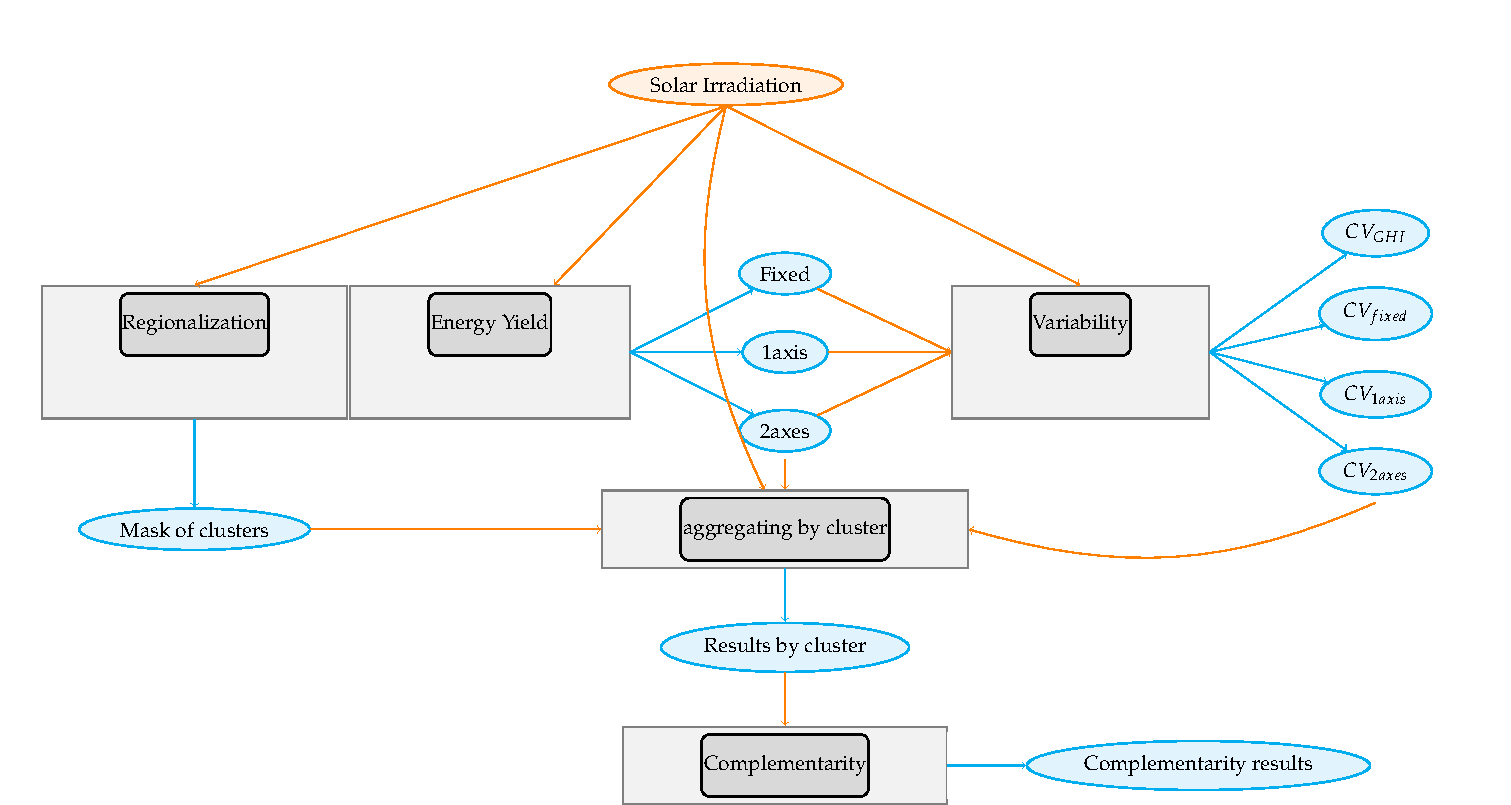
\includegraphics[width=1\textwidth]{figs/capitulo5/multi_step}
\caption[Stages of the multi-step scheme for variability and complementarity analysis]{Scheme: Each gray block represents each of the operations needed to get the variability and complementarity results. Orange ellipses are the data used and blue ellipses are the results of each stage. If the results of one of the blocks are used as input for another stage, connectors are represented in orange color.}
\label{fig:multi_step}
\end{figure}

\subsection{Regionalization by clustering}

Regionalization procedures provide the ability of extracting general information of the areas that could be treated as a coherent unit, facilitating the analysis and not considering those characteristics that are not under study. As it was explained in the methodological chapter, classical climatological classifications have some grade of subjectivity due to the fact that they rely on arbitrary assumptions \cite*{Kottek2006} and their criteria are based on temperature and precipitation \cite*{trewartha1980koppen}. For our purpose, objective and data-derived criteria are more suitable due to the fact that a different variable is analyzed and its classification does not match classical climate divisions. Objective methods based on clustering techniques have been applied successfully over the literature for the analysis of renewable energy resources \cite*{Polo2015}, \cite*{Zagouras2013}, \cite*{Zagouras2014}, \cite*{Zagouras2014b}, \cite*{gomez2015characterization} and atmospheric variables \cite*{Argueso2011}, \cite*{garcia2012seasonal}. 

% Clustering methods \cite*{Jain1999} can be divided into two categories, partitional and non-partitional. The partitional clustering divides the data into non-overlapping clusters while, the non-partitional or hierarchical clustering, provides a set of nested clusters. In our case, we made use of both algorithms selecting the hierarchical method to initiate a partitional algorithm that is the most suitable for our purpose: to find spatial regions that group together similar time series of the variable analyzed.

A commonly applied regionalization methodology includes the K-means algorithm after preprocessing the data through Principal Component Analysis \cite*{Ding2004}. This two-step method first reduces redundant information by a Principal Component Analysis that decreases dimensionality of the original dataset. After that, K-means algorithm is applied to the reduced data to find the optimal partition of clusters, which is based on similarity between each element or object inside the cluster and its centroid. This is considered as the most representative element of the cluster, and similarity is measured by an objective function defined in the cluster algorithm.

This method presents some problems regarding the random selection of the cluster centroids in the first step. Different initial centroids can lead to different solution or a local optimum could be found. Also, there could be some computational problems if many iterations are needed to get the final partition.

The procedure used in \cite{Argueso2011} and in \cite{Zagouras2014} is adapted to get the optimal partition in our scheme from a combined clustering grouping and avoiding the above mentioned problems: the \textbf{K-means partitional algorithm is initialized with a hierarchical clustering solution of the dimension-reduced data by a Principal Component Analysis.} For the particular case applied in this work, vectors of daily solar irradiation are used for the regionalization. The following steps are needed to get the optimal partition of clusters in the area:

\begin{itemize}
\item \textbf{To reduce data dimensionality}. Principal components are eigenvectors of an orthogonal matrix after applying a singular value decomposition (SVD) to the original data, daily solar irradiation vectors, whose initial dimension is reduced to the first eigenvectors that retain $95\%$ of the variance. Considering that, a linear combination of these eigenvectors represents the initial data.
\item \textbf{Hierarchical clustering to initialize k-means}. A hierarchical clustering method classifies data based on a hierarchy. If it is agglomerative, it will start with a cluster for each observation of the data and observations will group together recursively by similarity using the “complete linkage” method. Once the hierarchy is obtained, centroids can be calculated for each emerged partition with a number of clusters between 2 and \textit{n}, where \textit{n} is a high enough selected number of clusters. Centroids will be the initial seed for the Kmeans algorithm, avoiding the computational problems and favoring reproducibility.
\item \textbf{K-means algorithm}. The K-means algorithm is a partitional clustering method that minimizes an objective function that defines similarity among the elements of each cluster. In our case we made use of the Euclidean distance, Eq. \ref{eq:euclidean} between the objects or elements in the cluster, $x_{i}$, and its centroid, $c_{j}$, as the objective function. The number of clusters in which the data is divided into has to be known beforehand. In order to overcome the inconvenience, the algorithm is run from 2 to \textit{n} clusters and the optimum number is determined by making use of a clustering validity index after that.

\begin{equation}\label{eq:euclidean}
    J =\sum_{i=1}^{k}\sum_{j=1}^{n}{||x_i-c_j||}^2
\end{equation}

\nomenclature[J]{$J$}{Objective function of the Kmeans clustering method: summation over euclidean distances}
\nomenclature[x_i]{$x_i$}{Each point in the cluster, where the point is a vector with elements comprising the daily irradiation time series values at a pixel obtained from satellite images }
\nomenclature[c_j]{$c_j$}{Centroid of the cluster j}
%\nomenclature[PV]{$PV$}{Photovoltaic}
\nomenclature[IP]{$IP$}{Iberian Peninsula}

\item \textbf{Validity index}. In order to determine the optimal partition, validity clustering techniques are applied. There are two types of validation for the clustering methods. First, external clustering validation methods that make use of external information out of the data; and secondly, there are internal clustering validation methods that rely only on information from the data \cite*{Liu2010}. The latter are used to preserve objectivity as much as possible and are based on two criteria: compactness and separation of the clusters emerged. We use one of the most applied validity indices, the Calinski-Harabasz index \cite*{CalinskiH}, CH, that evaluates the average between and within cluster sums of squares.
\item \textbf{L-method}. CH index is calculated for every partition from 2 to $n$ clusters. The resulting CH graph in Figure \ref{CHindex} for the Iberian Peninsula regionalization is shown for a number of clusters between 2 and 70 as an example. Theoretically, the partition with the maximum CH is the optimum, but the graph shows a decreasing trend which leads to imprecision in finding the optimum. The large number of data and the continuous variable analyzed are responsible for that. For that reason, the L-method is applied \cite*{Salvador2004}. This method selects the intersection of two best-fit lines in the graph CH vs. \textit{k}, where \textit{k} is the number of clusters of the partition \cite*{Zagouras2013}. All possible pairs of lines that fit linearly to the left and right sequence of data points are created. Each line has at least two points. The total root mean squared error is calculated as in Eq.:\ref{eq:total_RMSE}:

\begin{figure}[h!]
\centering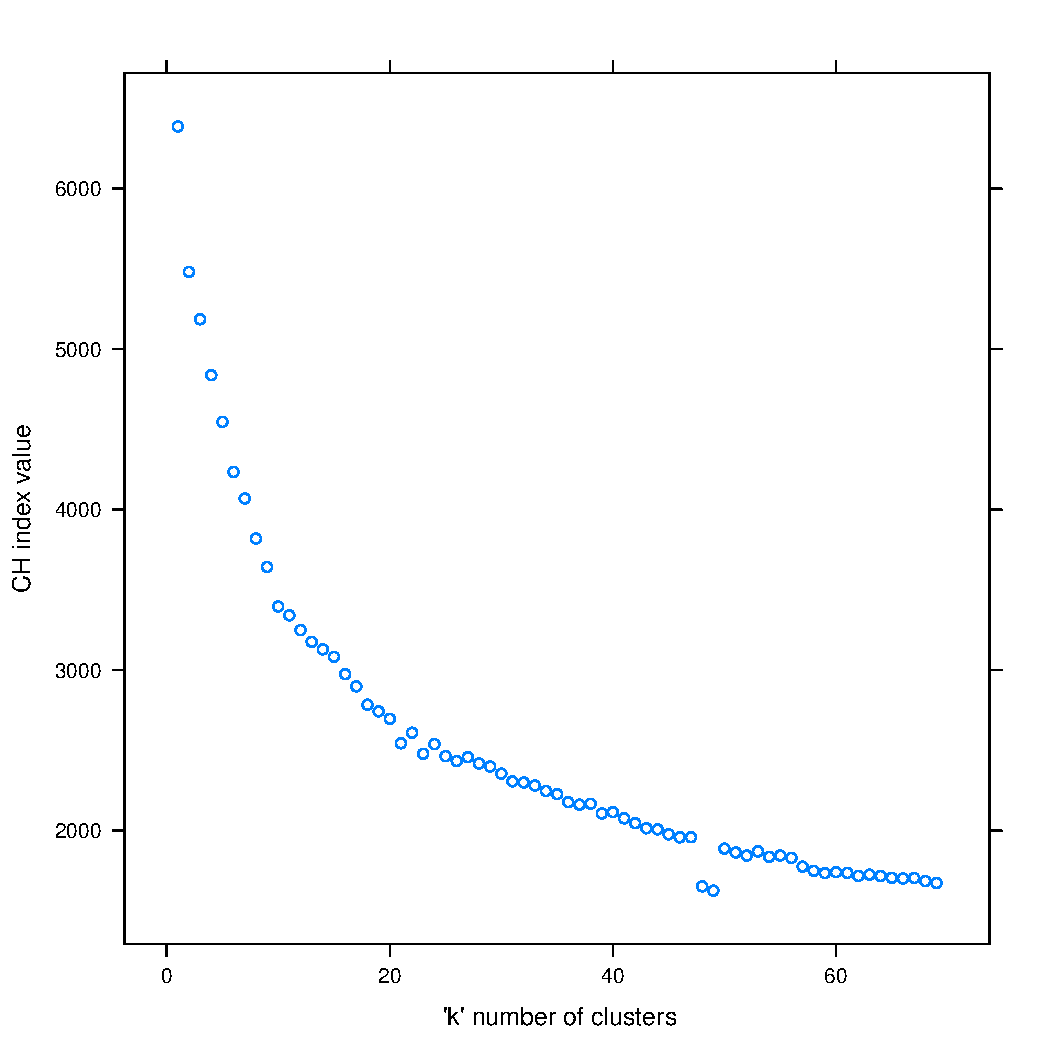
\includegraphics[width=0.5\textwidth]{figs/capitulo5/CHindex}
\caption[Calinski-Harabasz index by number of clusters]{Calinski-Harabasz index by ``k'' number of clusters}
\label{CHindex}
\end{figure}
 
\begin{equation}\label{eq:total_RMSE}
  RMSE_T = \frac{c-1}{k-1}RMSE_{left}+\frac{k-c}{k-1}RMSE_{right}
\end{equation}


\nomenclature[k]{$k$}{number of clusters.}
\nomenclature[c]{$c$}{number of clusters where the 2 fit-lines split.}
\nomenclature[CH]{$CH$}{Calinski-Harabasz validity index.}
\nomenclature[RMSET]{$RMSE_T$}{Total root mean square error.}
\nomenclature[RMSEleft]{$RMSE_{left}$}{Root mean squared error of the left-side linear regression.}
\nomenclature[RMSErigth]{$RMSE_{right}$}{Root mean squared error of the right-side linear regression.}

Where \textit{c} is the number of clusters where the graph is split into the two fit-lines, \textit{k} is the total number of clusters. The ``total root mean square error'' is a weighted error with two terms, one for each side of c in the graph. Each side has a heavier weight depending on the points involved in the fitting. The minimum of $RMSE_{T}$ gives us the optimum number of clusters of the data \cite*{Zagouras2013} which are used in the following steps.
 
\end{itemize}
 
\subsection{Photovoltaic energy yield}

The simulation of a photovoltaic energy system is carried out in two steps, as described in a previous chapter. The method is summarized here in order not to miss the coherence of the text.


\begin{enumerate}

\item In first place, global irradiation at the horizontal plane, $G(0)$, is transformed into the plane-of-array irradiation,  $G(\alpha, \beta)$, where $\alpha$ is the azimuth angle and $\beta$ the inclination angle of the generator plane. Due to optical losses (reflection, angle of incidence, and dust), the irradiation available is reduced for the photovoltaic cells inside the panels and the plane-of-array irradiation is then denoted as effective irradiation on the PV generator $G_{eff}(\alpha, \beta)$.
Three different types of tracking types are considered for the photovoltaic generator, which affect the tilt of the panels:
\begin{itemize}
\item \textbf{Fixed}: panels with an optimum angle of inclination that depends on the latitude of the place.
\item \textbf{One Axis}: North-South oriented panels that track the sun daily varying the azimuth angle.
\item \textbf{Two-axes}: tracking system that allows variation of the azimuth and inclination angles.
\end{itemize}
  
\item Once the effective irradiation that reach solar cells has been assessed, the second step is the transformation into power output that depends on the photovoltaic system. The photovoltaic system is composed of a PV generator, consisting of several PV modules, and an inverter to transform the DC current output from the generator into AC current to be integrated into the network. %In order to estimate  potential for photovoltaic production, the term \textit{yield} is defined as the system energy produced divided by the power installed $[\si{\kilo\watthour\per\kilo\wattpeak}]$.

\end{enumerate}

\subsection{Variability and complementarity}

The metric to analyze interannual variability is the coefficient of variation, CV (Eq.\ref{eq:CV}), which is defined as:

\begin{equation}\label{eq:CV}
  CV=\frac{\sigma}{\overline{X}}
\end{equation}

In this equation, $\sigma$ is the standard deviation of the variable analyzed and it is divided by the mean of the variable in the period of the study. Sometimes CV is represented in percentage. This measure is dimensionless and can be applied in different time scales, which is helpful for comparisons.

To assess complementarity of the solar resource in the area of study, the Pearson's correlation coefficient between the time series of pairs of clusters is calculated, Eq. \ref{eq:pearson}. Different aggregation time steps for the time series (daily, monthly, etc.) can be selected to assess complementarity in different time scales. 

\begin{equation}\label{eq:pearson}
  \rho_{i,j}=\frac{\sigma_{c_i,c_j}}{\sigma_{c_i}\sigma_{c_j}}
\end{equation}

In this equation, $c_i$ and $c_j$ are the time series corresponding to the clusters $i$ and $j$.

For a spatial complementarity analysis the range of the area studied has to be taken into account. The area must be large enough to make sense of the comparison between zones, due to the fact that geographically dispersed areas, far from each other, will have very different evolution of atmospheric variables. At the same time, large areas may not be interesting from the electricity generation point of view if, for instance, they are different networks without any market interaction. On the other hand, if the area of study is too small, atmospheric variables and therefore, renewable resources will evolve in a very similar way. For such small areas, local complementarity between different resources can be analyzed, but spatial complementarity of one resource cannot.

The correlation coefficient for an entire long time series may hide changes in complementarity for shorter sub-periods. For that reason a moving correlation window can be applied, in order to provide an indication of how correlation between clusters varies during the whole period. Width of the window is selected depending on the case under study and the time scale evaluated. For some studies, it can be interesting to assess weekly variations of the correlation coefficient between areas, whereas in other cases, it is more important to consider lower frequency variations in the complementarity.

A 15 years moving window is selected over a 30-years monthly time series in order to look for higher frequency changes in the correlation coefficient patterns inside the entire period. Thus, a collection of correlation coefficients by month for each pair of clusters will be obtained. In order to detect the most important cluster pairs regarding complementarity, the median of the whole set of correlation coefficient series is calculated for each pair of clusters. Then, the  sorted coefficients will indicate the cluster pairs that reach lower values of correlation being potentially interesting for the spatial complementarity.

% In order to obtain the more important cluster pairs regarding complementarity, the median of the correlation coefficient series is calculated for each pair. After that, the cluster pairs are reordered from lower to higher values of this median correlation.
%, and the first 15 pairs (with the lowest median correlation) are selected as the most representative of complementarity, altought this number is rather arbitrary and also depend on the length of the time-series analysed.
 

\section{Results}

\subsection{Regionalization}

The optimal partition after having applied the clustering method is represented in Figure \ref{clusters}. The CH validation procedure gives an optimum number of 19 clusters for the area, where each of the clusters has an homogeneous time evolution of solar irradiation. Due to the nature of clustering techniques, there is not a unique/best method to select the optimum partition. Another index (Davies-Boudin, \cite{davies1979cluster}) has been applied for comparison, and the obtained optimum number of clusters was of the same order than for CH index.
 
\begin{figure}[h!]
\centering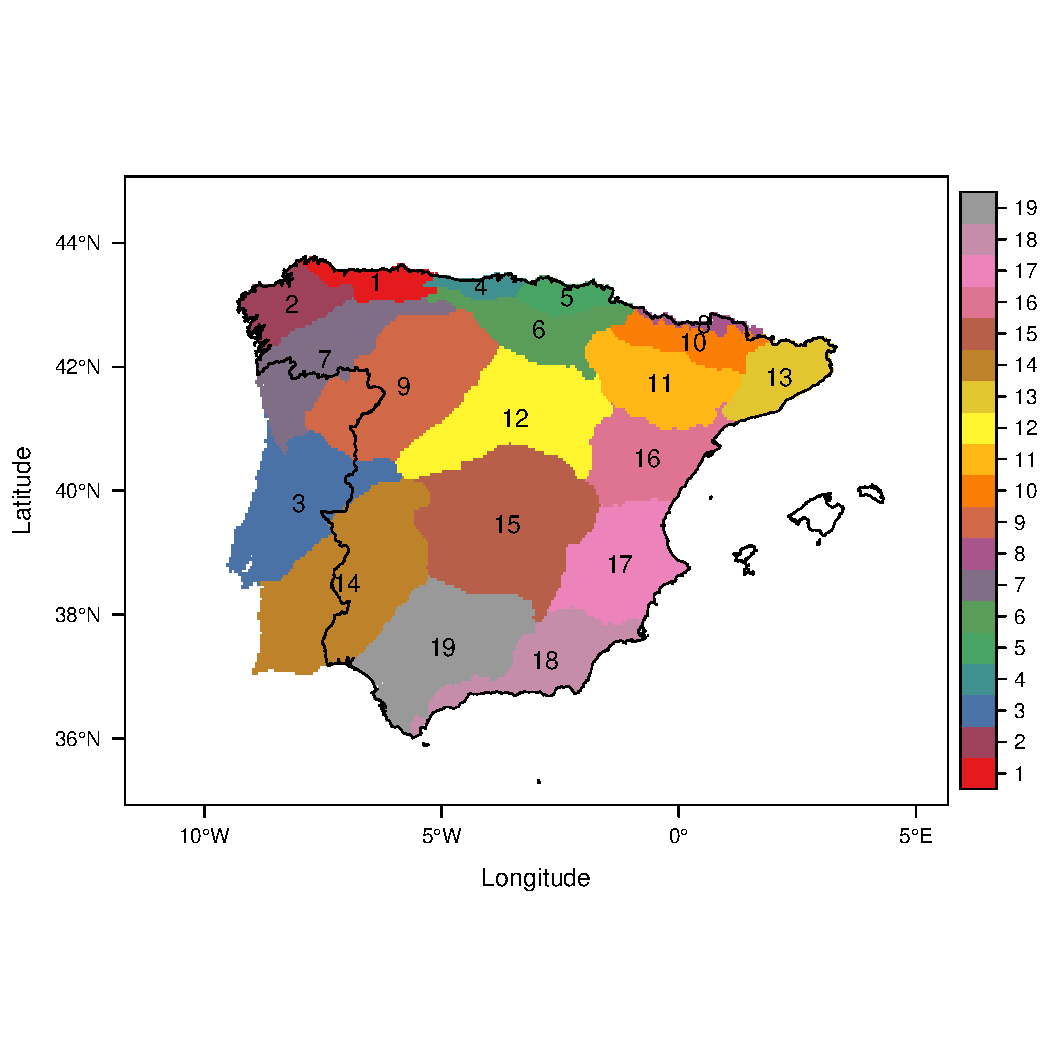
\includegraphics[width=0.6\textwidth]{figs/capitulo5/clusters2}
\caption[Optimal partition of clusters over the Iberian Peninsula]{Optimal partition of 19 Clusters after applying the algorithm and the validity index. Geographically clusters can be roughly divided: north-west (2,7), north (1,4,5,6), Pyrenees (8), north-east (10,11,13,16), south-east (17,18), centre-north (9,12), west (3), centre-south (14,15,19)}
\label{clusters}
\end{figure}

  
The ability of the clustering method to select optimum regions and to represent different climates of the area can be highlighted evaluating aggregated values of yearly mean of daily irradiation by cluster. Higher values are found in clusters 14, 15, 17, 18, 19, as can be seen in Table \ref{tabla2} which corresponds to the southern half of the Iberian Peninsula. Apart from this latitude-related maximum irradiation, a particularly high value is found in cluster 11, clearly above all surrounding clusters in the northern half of the Iberian Peninsula. This cluster corresponds to the central Ebro basin, which is characterized by a very dry continental climate. It is a deep depression totally surrounded by mountain ranges like the Pyrenees,  which frequently cause a Föhn effect which reduces cloudiness and precipitation in comparison with other nearby clusters. Excluding this cluster, irradiation in the northern half of the Iberian Peninsula (1, 2, 3, 4, 5, 6) is lower than in the southern half, and the minimum values are found in clusters in the northern coast and the Pyrenees. The maximum solar irradiation is 50 percent higher than the minimum, which reflects the large climatic differences between clusters.

\begin{center}
  \begin{table}[h!]
\begin{tabular}{c|c|c|c|c|c|c|c|c}
Zone & $G(0)$ & $CV_{G0}$ & $Yf_{\rm Fixed}$ & $CV_{\rm Fixed}$ & $Yf_{\rm One}$ & $CV_{\rm One}$ & $Yf_{\rm Two}$ & $CV_{\rm Two}$ \\
\hline
1 & 3.4 & 3.6 & 1047 & 4.2 & 1225 & 4.9 & 1381 & 5.1\\ 
2 & 3.8 & 3.2 & 1120 & 3.6 & 1359 & 4.3 & 1520 & 4.6\\
3 & 4.6 & 2.8 & 1350 & 3.4 & 1720 & 3.7 & 1921 & 4.1\\
4 & 3.4 & 4.1 & 1024 & 4.7 & 1198 & 5.4 & 1351 & 5.7\\
5 & 3.4 & 4.2 & 1035 & 4.7 & 1226 & 5.5 & 1374 & 5.8\\
6 & 4.0 & 3.2 & 1190 & 3.7 & 1465 & 4.2 & 1640 & 4.5\\
7 & 4.1 & 3.4 & 1224 & 3.9 & 1530 & 4.4 & 1712 & 4.8\\
8 & 3.6 & 4.6 & 1099 & 6.3 & 1322 & 6.4 & 1473 & 7.5\\
9 & 4.5 & 2.7 & 1356 & 3.0 & 1725 & 3.5 & 1934 & 3.8\\
10 & 4.4 & 2.7 & 1367 & 3.2 & 1696 & 3.6 & 1937 & 3.9\\
11 & 4.7 & 2.0 & 1404 & 2.6 & 1787 & 2.7 & 2024 & 3.1\\
12 & 4.5 & 2.6 & 1348 & 3.1 & 1701 & 3.5 & 1911 & 3.8\\
13 & 4.4 & 2.7 & 1340 & 2.9 & 1660 & 3.4 & 1893 & 3.7\\
14 & 4.9 & 2.2 & 1423 & 2.8 & 1837 & 3.0 & 2047 & 3.4\\
15 & 4.9 & 2.3 & 1427 & 2.9 & 1837 & 3.0 & 2057 & 3.4\\
16 & 4.5 & 2.6 & 1374 & 3.0 & 1722 & 3.4 & 1946 & 3.7\\
17 & 4.9 & 2.5 & 1429 & 2.9 & 1830 & 3.3 & 2052 & 3.6\\
18 & 5.1 & 2.4 & 1470 & 2.9 & 1906 & 3.2 & 2123 & 3.5\\
19 & 5.1 & 2.1 & 1456 & 2.8 & 1891 & 2.8 & 2105 & 3.7\\
\end{tabular}
\caption[Values of yearly mean of daily irradiation, yearly yield by tracking system and interannual CV of yearly mean by cluster over the Iberian Peninsula]{Values of yearly mean of daily irradiation $\left[\si{\kilo\watthour\over\metro^2}\right]$, yearly yield by tracking system $\left[\si{\kilo\watthour\over\kilo\wattpeak}\right]$ and interannual CV of yearly mean in percentage \%.}
\label{tabla2}
\end{table}
\end{center}

\subsection{Variability results}

After regionalization, an analysis of solar irradiation at the horizontal plane and PV yield by tracking system is performed, including their temporal variability.

Regarding interannual variability, we have calculated the CV of two time-aggregated means of solar irradiation and PV yield:

\begin{itemize}
\item On one hand it is applied for the yearly mean of daily irradiation $G_{d,y}(0)$ and yearly PV yield. This metric gives the variation of the energy from one year to another and if it is low, general stability of the solar resource and PV production is guaranteed. 
\item On the other hand the interannual variability of the monthly time series $G_{d,m}(0)$ and monthly energy yield is also investigated in order to quantify differences in the annual cycle. 
\end{itemize}

The CV is also aggregated by cluster, in order to facilitate the intercomparison among areas.

%The general results about yield and variability can be found in the appendix. Here we present particularly relevant results that show the importance of considering different types of tracking methods, which is a fundamental aspect of the proposed scheme.\\

% Power from the PV generator depends quasi-linearly with solar irradiation at the plane-of-array ($G_{eff}(\alpha,\beta)$), besides second order effects (spectrum, wind, etc) \cite*{Perpinan2007} . Due to that the fixed typology is the one with lower yield because the amount of irradiation reaching cells is lower than the amount of energy reaching panels when trackers have one or two axes movements.

\subsubsection{Yearly mean}

The results for the CV of the yearly mean of daily irradiation and of the annual mean yield by tracking type, aggregated by cluster, are shown in Table \ref{tabla2}. Also, yearly mean of daily irradiation is represented, showing differences in resource among areas, as well as yield differences.

The highest values of CV (above $4\%$) are seen in clusters 8, 4 and 5. These clusters correspond to the Pyrenees and the northern Cantabric coast. This behavior can be explained in part through the influence of variable summer cloudiness, as these areas are not affected by the summer dryness typical of the Mediterranean climate of most of the Iberian Peninsula. Southern and central regions are the least variable. Remarkably, the lowest value of CV is found in cluster 11, corresponding to the central Ebro basin, located at the north of the Iberian Peninsula. Very low values near $2\%$   are also found in the southwestern clusters (4 and 19), a result that coincides with \cite{Gil2015}. Finally, the north-western clusters (2 and 7) show a higher value than the northeastern cluster 13, despite sharing the same latitude. The north-western clusters are particularly influenced by the Azores high position and interannual variability.

Regarding the electricity production, power from the PV generator depends quasi-linearly on solar irradiation at the plane-of-array ($G_{eff}(\alpha,\beta)$), apart from second order effects (spectrum, wind, etc) \cite*{Perpinan2007} . Due to that, the fixed typology is the one with lower yield because the amount of irradiation reaching cells is lower than the amount of energy reaching panels when trackers are allowed to move in one or two axes.

For areas where solar irradiation is higher, yield differences between trackers are higher. This can be seen in Figure \ref{yearly_productivity_byCluster} where yearly mean yield for the 30-years period is aggregated by cluster and tracking system, and clusters are sorted vertically from less to more energy yield. Yield increase from fixed panels to one-axis panels is non-linear. This increase ranges between $17\%$ for the clusters with less solar irradiation, located at the northern coast like clusters 4, 5; and $30\%$ for the southern clusters with more solar irradiation (clusters 18, 19). In contrast, energy yield increase from one-axis to two-axes panels is almost constant, around $12\%$ for all clusters. A consequence of the non-linear PV yield increase from fixed to one-axis panels is that the energy yield differences between clusters are much higher for tracking than for fixed systems. While for fixed panels PV energy yield varies between 1000 and 1450 $\left[\si{\kilo\watthour\over\kilo\wattpeak}\right]$, for two-axes systems it varies between 1350 and 2100 $\left[\si{\kilo\watthour\over\kilo\wattpeak}\right]$. These average values are coherent with results obtained in \cite{Antonanzas-Torres2013}.
 
\begin{figure}[!tbp] 
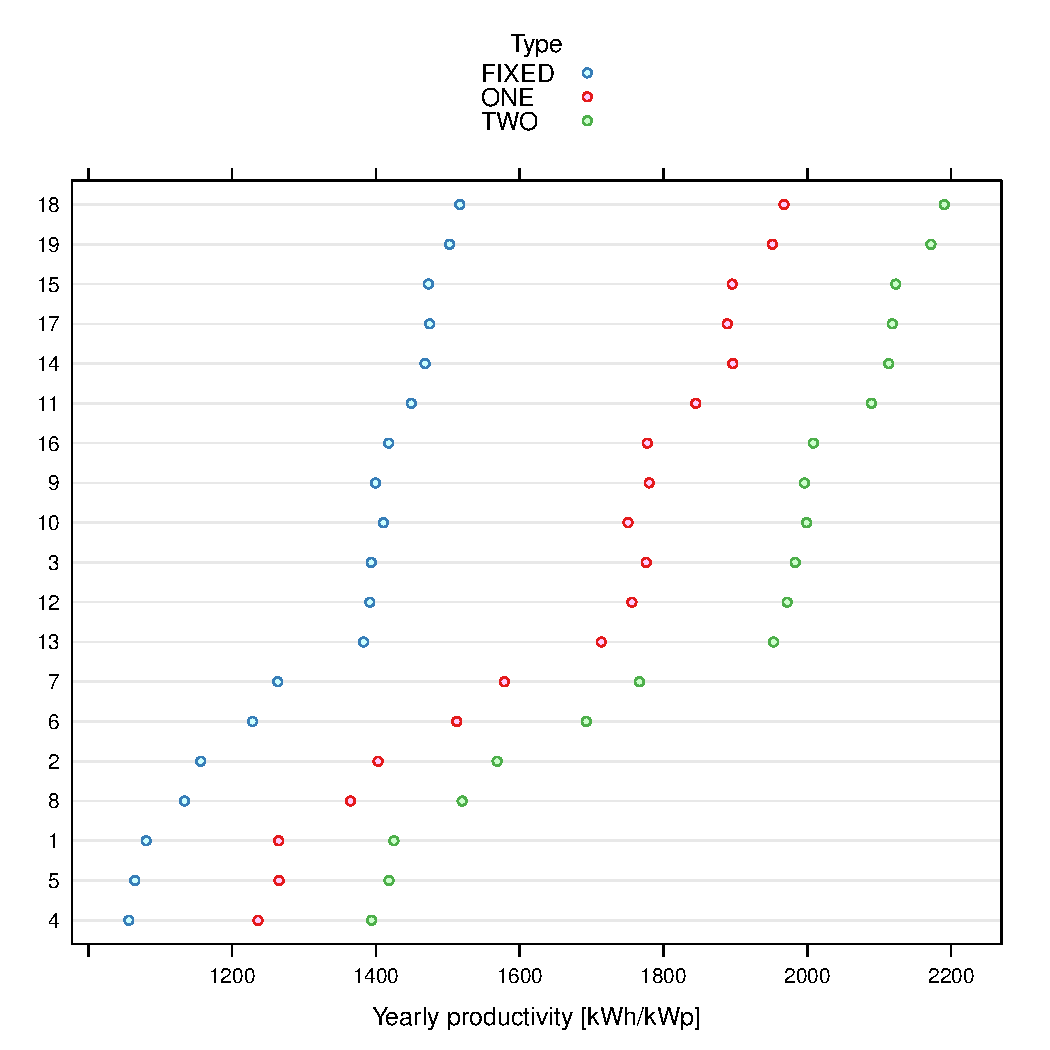
\includegraphics[width=0.7\textwidth]{figs/capitulo5/productivity_bycluster_andtype.pdf}
\caption[Yearly mean of PV yield by cluster and tracking type over the Iberian Peninsula]{Yearly mean of PV yield by cluster and for each tracking system $\left[\si{\kilo\watthour\over\kilo\wattpeak}\right]$. Values are sorted from lower to higher yield values.}
\label{yearly_productivity_byCluster}
\end{figure}

\subsubsection{Monthly mean}

Variations in electricity prices from one year to another are significantly dependent on the interannual variation of the monthly renewable electricity production. This time-scale is also mostly influenced by the large scale circulation modes for solar potential in the Iberian Peninsula \cite*{Jerez2013a} and the winter half of the year, from October to March, is especially variable.

\begin{figure}
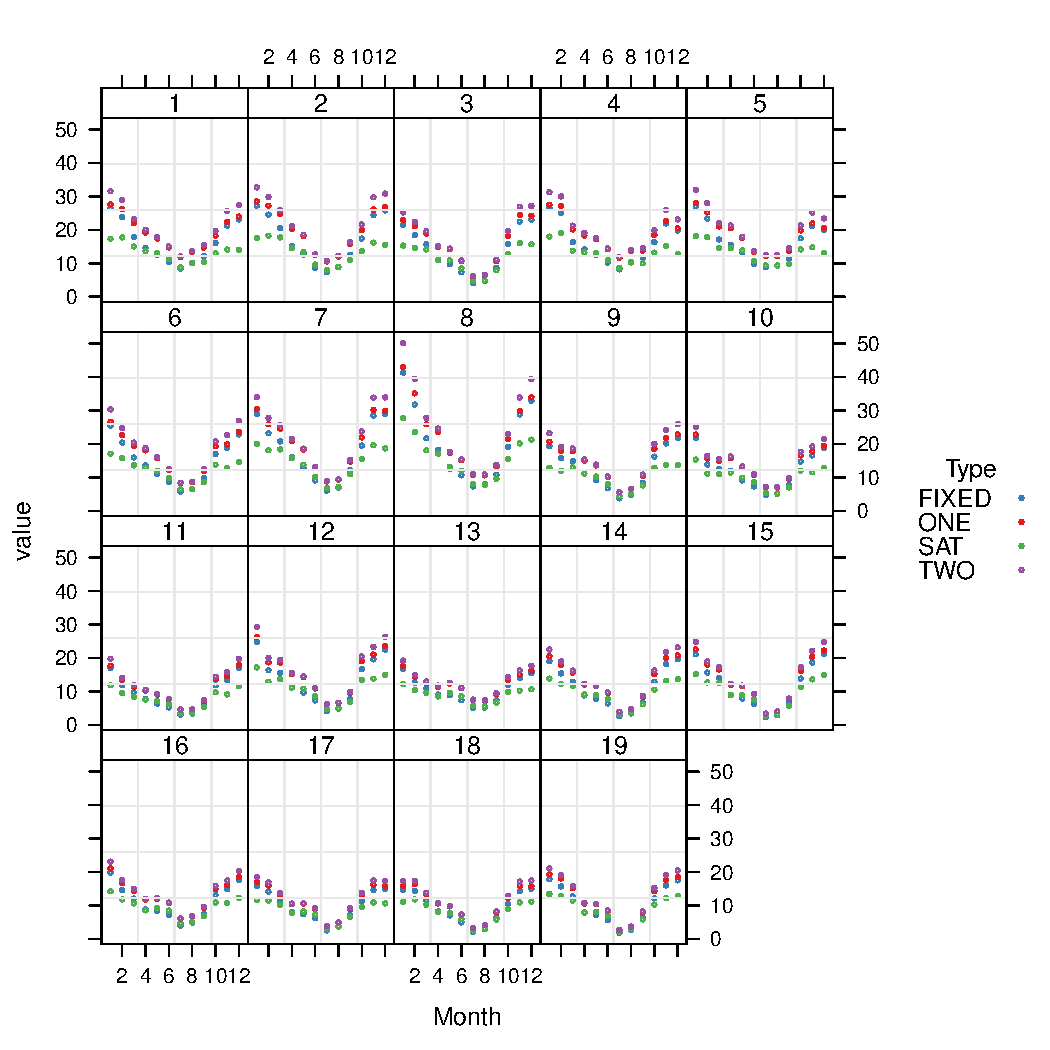
\includegraphics[width=0.8\textwidth]{figs/capitulo5/ciclo_anual_byCluster_all2}
\caption[Annual cycle of CV by cluster and tracking type over the Iberian Peninsula]{Annual cycle of CV ($\%$) by cluster and for each tracking type and global solar irradiation at the horizontal plane.}
\label{cicloAnualCV_all}
\end{figure}

Annual cycles of interannual monthly CV are represented in Figure \ref{cicloAnualCV_all}. The interannual variability for monthly yield is higher than for the solar irradiation at the horizontal plane. In winter months, these differences in CV are much higher than in summer. This behavior is more pronounced in northern areas (clusters 1, 2, 3, 4, 5, 6, 7).  Seasonal patterns can be appreciated in all the areas although some clusters in the north-east area (13, 11) present flatter cycles.

Regarding solar irradiation variability, it is also important to notice the differences in winter months between the eastern and north-western sides of the Iberian Peninsula. Eastern clusters (10, 11, 13, 16, 17, and 18), have smaller values of CV (below $15\%$) in winter than northern and north-western clusters (1, 2, 3, 4 and 7), where values above $15\%$ and close to $20\%$ are found. In summer there is a different behavior because the main differences exist between the north and the south of the Iberian Peninsula. Northern clusters (1, 2, 4, 5 and 8) show summer CV values above $7\%$, while southern clusters (15, 14, 17, 18 and 19) show very low values, around $2\%$.

Cluster 8, in the Pyrenees region has the highest values in winter, above $25\%$. Its annual cycle has a wide range between winter and summer, decreasing to $7\%$ in August. On the other hand, north-eastern clusters (13, 11, and 10) show the smallest differences between winter and summer for the CV of solar irradiation.

In order to quantify differences in variability between solar irradiation and solar power output, the ratio between variability of yield by tracking system and solar irradiation is represented in Figure \ref{ratiosCV} for each month and cluster. If CV of energy yield is higher than CV of solar irradiation, values are above one. On the other side, values will be below one if CV of solar irradiation is higher than CV of energy yield. 

\begin{figure}
  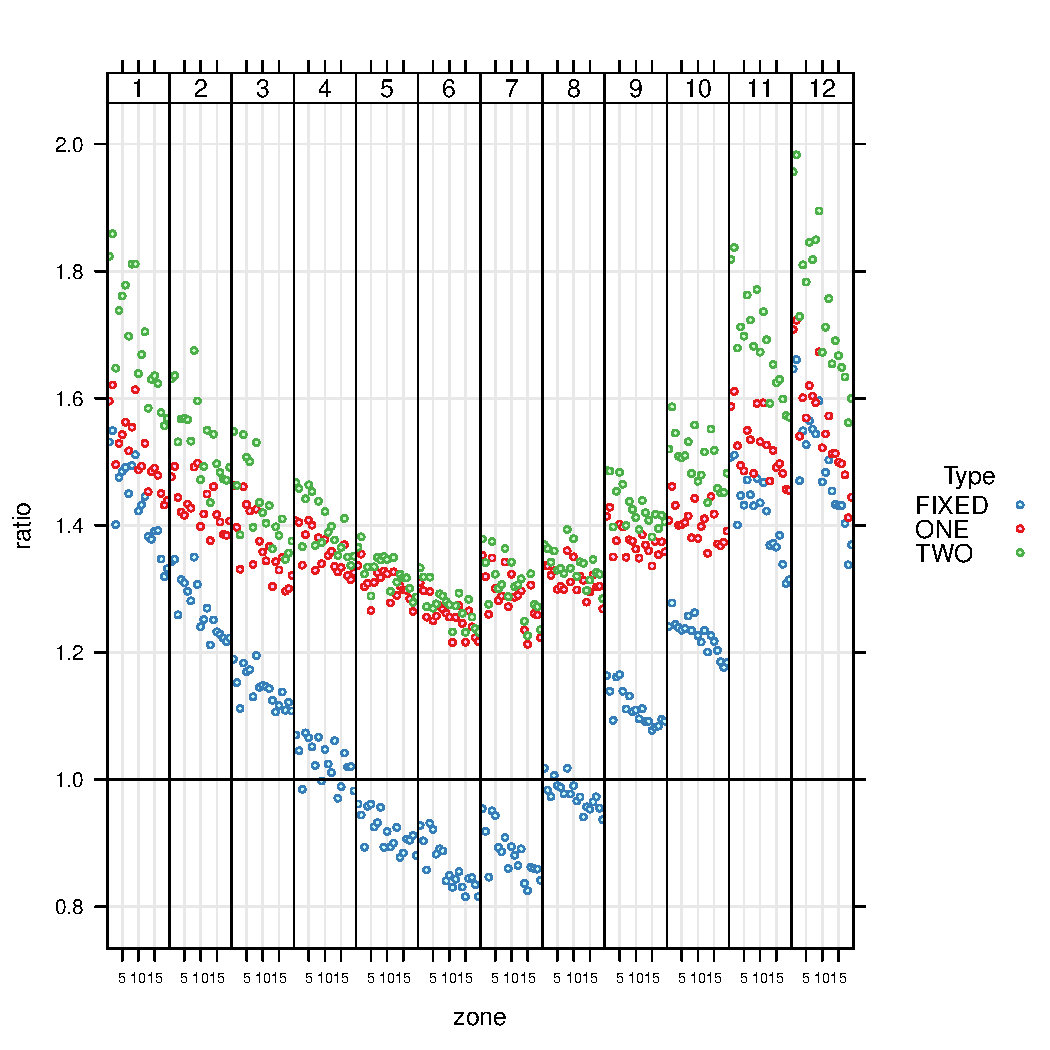
\includegraphics[width=0.7\textwidth]{figs/capitulo5/dotplot_ratio_zone2.pdf}
  \caption[CV ratios of PV by tracking type and solar irradiation at horizontal plane]{CV ratios between each type of tracking system and solar irradiation at the horizontal plane, grouped together by month in the graph. Ratios are calculated for each cluster, represented in the x axis. ``Fixed'' represents $\frac{CV_{\rm Fixed}}{CV_{G0}}$, ``One'' is $\frac{CV_{\rm One}}{CV_{G0}}$ and ``Two'' is $\frac{CV_{\rm Two}}{CV_{G0}}$}
  \label{ratiosCV}
\end{figure}

The highest ratios are obtained between $CV_{\rm Two}$ and $CV_{G0}$. The ratio of $CV_{\rm One}$ is clearly lower in winter months, but in summer it is very similar to the ratio of $CV_{\rm Two}$. Yield with a 'horizontal' axis tracker and 'two-axes' trackers increase the variability between $20\%$ in summer and more than $80\%$ in some areas in winter. The fixed typology ratio, $CV_{\rm Fixed}/CV_{G0}$ has a much wider range in the whole year. In winter months, it has values between 1.2 and 1.6, depending on the cluster, and is not far from the other two typologies. In contrast, this ratio decreases rapidly in summer months, reaching values below one between May and August. This means that for that period, variability of the ``fixed yield'' is smaller than variability of solar irradiation at the horizontal plane.

The results of CV show that variability of PV energy yield at tilted panels is higher than variability of solar resource at the horizontal plane in most cases, which can be explained by the nature of solar irradiation at tilt panels and its dependency of solar irradiation at the horizontal plane \cite{Perpinan2009}.

%\nomenclature[CV]{$CV$}{Coefficient of variation.}

% For areas where solar irradiation is higher, yield differences between trackers are higher. This can be seen in figure \ref{yearly_productivity_byCluster} where yearly mean yield for the 30-years period is aggregated by cluster and tracking system, and clusters are sorted vertically from less to more energy yield. A noteworthy result is that yield increase from fixed panels to one-axis panels is non-linear. This increase ranges between $17\%$ for the clusters with less solar irradiation, located at the northern coast (clusters 4, 5), and $30\%$ for the southern clusters with more solar irradiation (clusters 18, 19). In contrast, enegy yield increase from one-axis to two-axes panels is almost constant, around $12\%$ for all clusters. A consequence of the non-linear PV yield increase from fixed to one-axis panels is that the energy yield differences between clusters are much higher for tracking than for fixed systems. While for fixed panels PV energy yield varies between 1000 and 1450 $[\si{\kilo\watthour\over\kilo\wattpeak}]$, for two-axes systems it varies between 1350 and 2100 $[\si{\kilo\watthour\over\kilo\wattpeak}]$. These average values are coherent with results obtained in \cite{Antonanzas-Torres2013} when considering a value of 0.75 for the system performance ratio.
 
% \begin{figure}[!tbp] 
% 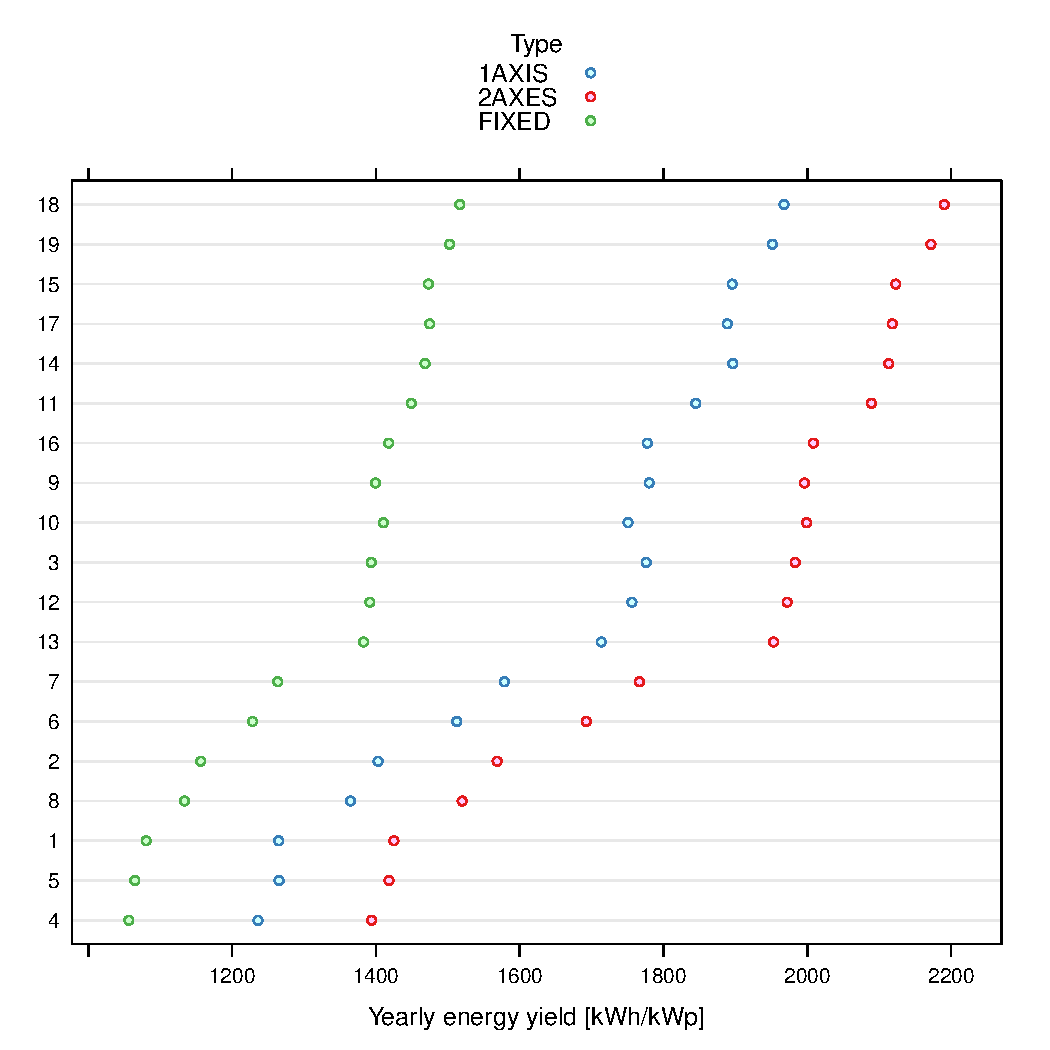
\includegraphics[width=0.6\textwidth]{figs/capitulo5/productividadTemp_byCluster.pdf}
% \caption{Yearly mean of PV yield by cluster and for each tracking system $[\si{\kilo\watthour\over\kilo\wattpeak}]$. Values are sort from lower to higher yield values.}
% \label{yearly_productivity_byCluster}
% \end{figure}

% Electricity price variations significantly depend on the variations of the monthly renewable electricity production from year to year. This time-scale is also the most influenced by the large scale circulation modes for solar potential in the Iberian Peninsula \cite*{Jerez2013a}. The winter half of the year, from October to March, is especially variable.

% The interannual variability for monthly yield is higher than for the irradiation at the horizontal plane, as it occurred for yearly values which results are in the appendix. In winter months, these differences in CV are much higher than in summer. This behavior is more pronounced in northern areas.

% In order to quantify these differences in variability between solar irradiation and solar power output, the ratio between variability of yield by tracking system and solar irradiation is represented in figure \ref{ratiosCV} for each month and cluster. If CV of energy yield is higher than CV of solar irradiation, values are above one. On the other side values will be below one if CV of solar irradiation is higher than CV of energy yield. 

% \begin{figure}
%   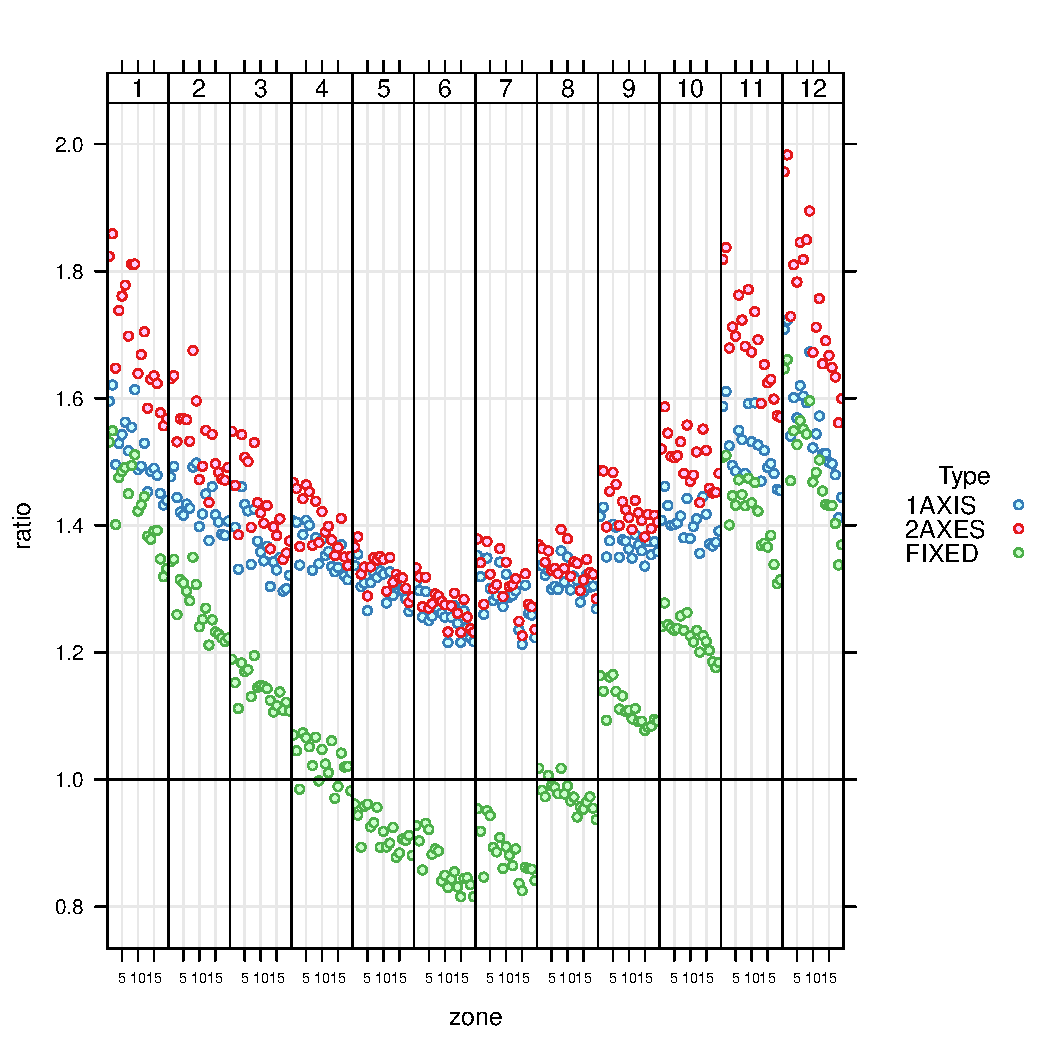
\includegraphics[width=0.6\textwidth]{figs/capitulo5/dotplot_ratio_zone.pdf}
%   \caption{CV ratios between each type of tracking system and solar irradiation at the horizontal plane, grouped together by month in the graph. Ratios are calculated for each cluster, represented in the x axis. ``Fixed'' represents $\frac{CV_{fixed}}{CV_{G0}}$, ``1 axis'' is $\frac{CV_{1axis}}{CV_{G0}}$ and ``2 axis'' is $\frac{CV_{2axes}}{CV_{G0}}$}
%   \label{ratiosCV}
% \end{figure}

% The highest ratios are obtained between $CV_{2axes}$ and $CV_{G0}$. The ratio of $CV_{1axis}$ is clearly lower in winter months, but is very similar in summer to the ratio of $CV_{2axes}$. Yield with an 'horizontal' axis tracker and 'two-axes' trackers increase the variability between $20\%$ in summer and more than $80\%$ in some areas in winter. The fixed typology ratio, $CV_{fixed}/CV_{G0}$ has a much wider range in the whole year. In winter months, it has values between 1.2 and 1.6, depending on the cluster, and is not far from the other two typologies. In contrast, this ratio decreases rapidly in summer months, reaching values below one between May and August. This means that for that period, variability of the 'fixed yield' is smaller than variability of solar irradiation at the horizontal plane.

% The results of CV show that variability of PV energy yield at tilt panels is higher than variability of solar resource at horizontal plane in most cases, explained by the nature of solar irradiation at tilt panels and its dependency of solar irradiation at horizontal plane, \cite{Perpinan2009}.

\subsection{Complementarity results}

The monthly time series are also selected for the complementarity analysis.
Regarding solar power complementarity, opposite-evolving time-series for different areas would strongly increase the reliability of the whole electric system, as shortfalls of solar irradiation in certain areas could be compensated by above-normal irradiation in others. However, this ideal situation is difficult to find in a rather limited area like the IP, at least for monthly time scales over a long time period of 30 years. In this case, the absence of correlation also becomes important, as it avoids simultaneous shortfalls or simultaneous above-normal values and therefore, softens the overall power production. Overall, the 30-year period correlation matrix for each month shows that southern and eastern clusters are uncorrelated at least during part of the year with northern and northwestern clusters. In some cases, the absence of correlation is found between nearby clusters. A more detailed discussion can be found in the appendix A.

It could be that the obtained clusters present higher complementarity in shorter sub-periods. As explained in section 5.3.3, we have divided the whole 30-year period in sub-periods of consecutive 15 years. The correlation coefficients have been calculated again for the resulting 15-year moving window, for each pair of clusters and for each month. In this way, we obtain how each correlation coefficient evolves during the 30 year period. The analysis has been applied for the four variables in the study: solar irradiation at the horizontal plane and PV energy yield for each tracking system.

The correlation coefficient evolution of the photovoltaic energy yield obtained with fixed panels and for the most important pair of clusters, in terms of complementarity (2-18), is represented in Figure \ref{series_correlacion} to illustrate main results. In addition, the less relevant pair of clusters (15-19), the one with the highest medium value of the correlation coefficient, is also overlapped in the Figure in order to show the differences that exist between the areas that present complementarity in some points of the period and those with high positive values for the whole time series.

Other relevant pairs for complementarity include a northern (1, 2, 4 or 5) and a south-eastern cluster (17 or 18),  although they are not shown in the graph. They behave similar to the pair 2-18, with a swinging time series that reaches negative values below -0.6 for the correlation coefficient at some 15-years sub-periods. 

\begin{figure}[h!]
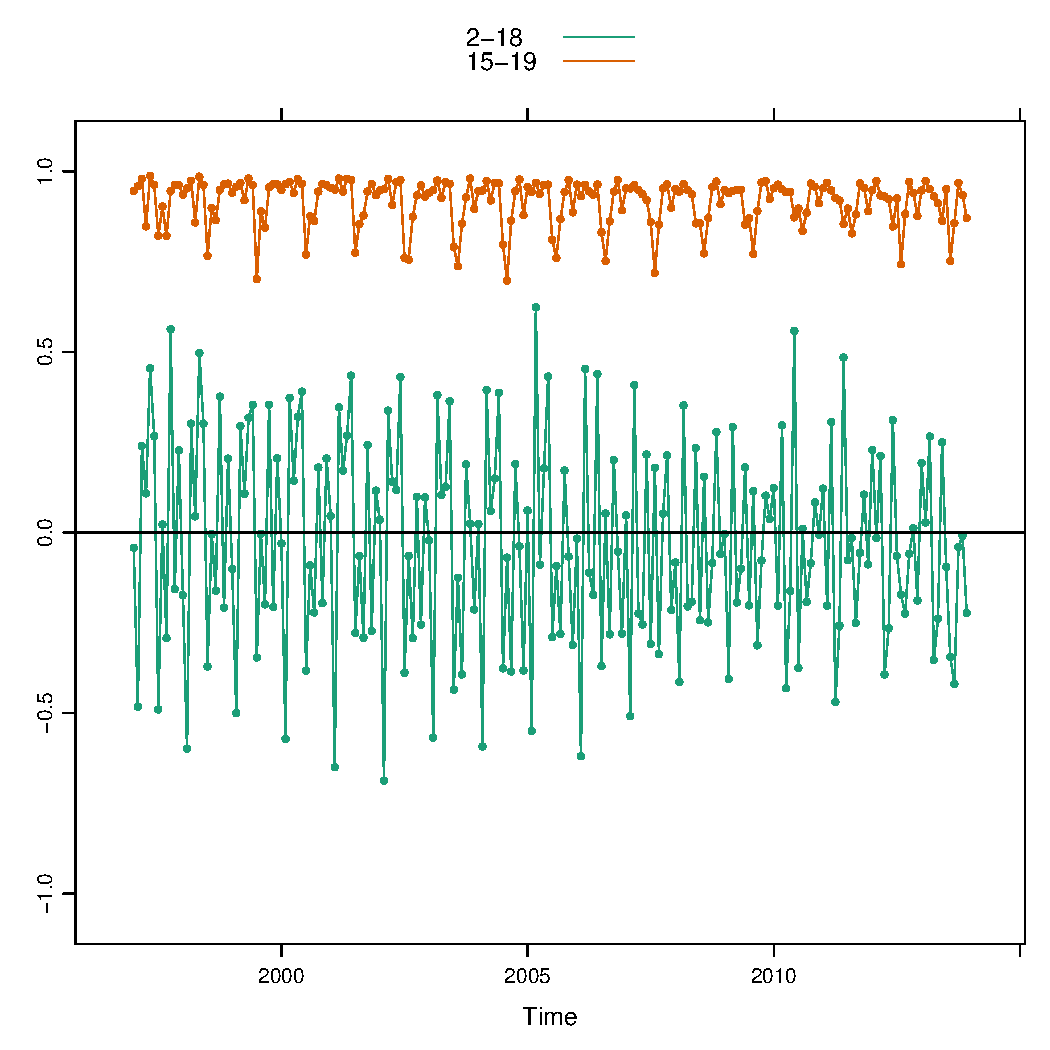
\includegraphics[scale=0.6]{figs/capitulo5/figure8.pdf}
\caption[Correlation coefficients of the yearly energy yield for the two pairs of clusters with the highest and smallest correlation values over the Iberian Peninsula]{Correlation coefficient of photovoltaic energy yield with fixed panels: evolution of a 15-year moving window of monthly values, for the first cluster pair showing the smallest median correlation value (2-18) and the latest with highest median correlation value (15-19).}
\label{series_correlacion}
\end{figure}

Among the first pairs in terms of complementarity, it is important to remark the appearance of 3-4 and 3-5 although they are not shown in the graph. These clusters are closer than the previously commented cases, which highlight the adequacy of the clustering method. All three are Atlantic coast clusters, but while cluster 3 includes part of the western coast, clusters 4 and 5 are northern coastal areas. This fact, together with the position of the main mountain ranges, can explain their partially complementary behavior.

In order to highlight the months with maximum anti-correlation, Figure \ref{series_correlacion_meses} presents, for the same cluster pairs as above, the minimum values of the monthly correlation coefficient (where the minimum for each month is calculated over all 15-year sub-periods). Differences between months are clearly observed in this graph. Only two months (March and June) show consistent positive values of this parameter and therefore, a low complementarity. In the other months, this parameter predominantly has negative values, revealing a certain degree of complementarity for the pair 2-18.

\begin{figure}[h!]
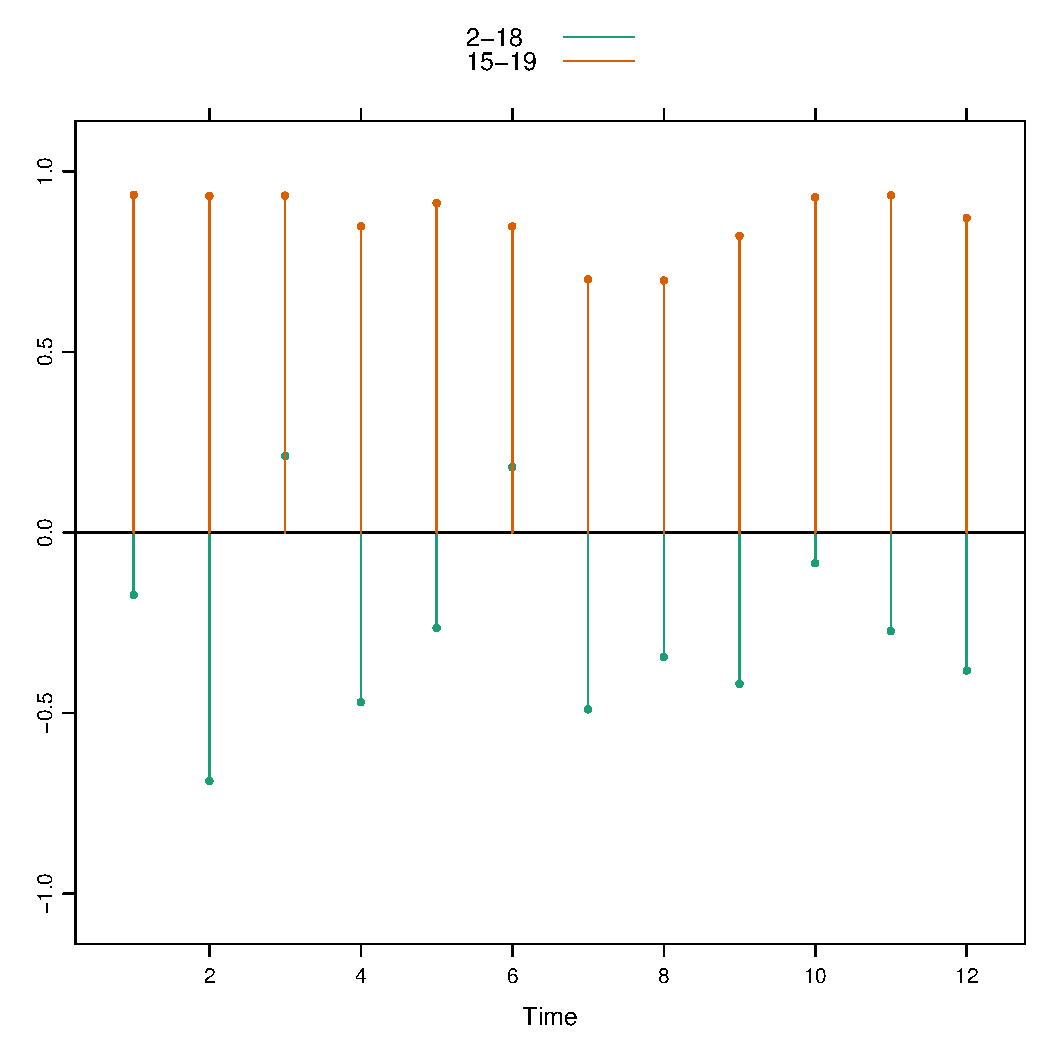
\includegraphics[scale=0.6]{figs/capitulo5/figure9.pdf}
\caption[Correlation coefficients of the monthly energy yield for the two pairs of clusters with the highest and smallest correlation values over the Iberian Peninsula]{Correlation coefficient of photovoltaic energy yield with fixed panels: minimum values of the monthly correlation coefficient, for the same cluster pairs as figure \ref{series_correlacion}. The minimum is calculated over all 15-year sub-periods.}
\label{series_correlacion_meses}
\end{figure}


% Regarding solar power complementarity, opposite-evolving time-series for different areas would strongly increase the reliability of the whole electric system, as shortfalls of solar irradiation in certain areas could be compensated by above-normal irradiation in others. However, this ideal situation is difficult to find in a rather limited area like the IP, at least for monthly timescales over a long time period of 30 years. In this case, the absence of correlation becomes also important, as it avoids simultaneous shortfalls or simultaneous above-normal values, and therefore softens the overall power production. The correlation matrix for the 30-year period and each month is in the appendix, showing the results for the whole period. In most cases, the correlation coefficient is highly positive, specially between pairs in the northern part of the Iberian Peninsula. For the southern part, the correlation coefficient is also positive but it decreases in July and August. There are some exceptions between the northern clusters 4 and 5 and the southern clusters 14 to 19, these pairs are only slightly correlated, not correlated or even slightly anticorrelated for some months.

% Overall, southern and eastern clusters are uncorrelated at least during part of the year with northern and northwestern clusters. In some cases, the absence of correlation is found between nearby clusters: in winter months, the north-eastern cluster 11 (central Ebro valley) is uncorrelated to the closely-lying clusters 4, 5 and 8 (in the northern coast and Pyrenees). This is probably related to persistent atmospheric situations with north to northwesterly winds, that cause cloudiness in the windward clusters and clear skies in the leeward Ebro cluster, due to a foehn effect. This result points out the selective character of the clustering method.

% It could be that the obtained clusters present higher complementarity in shorter sub-periods. We have divided the whole 30-year period in sub-periods of consecutive 15 years. The correlation coefficients have been calculated again for the resulting 15-year moving window, for each pair of clusters and for each month. In this way, we obtain how each correlation coefficient evolves during the 30 year period. The analysis has been applied for the four variables in the study: solar irradiation at the horizontal plane and PV energy yield for each tracking system.

% The median value of the correlation coefficient series is calculated for each pair. Each serie comprises 12 monthly values for each of the 15-year moving windows. After that, the cluster pairs are reordered from lower to higher values of this median correlation, and the first 15 pairs (with the lowest median correlation) are selected as the most representative of complementarity. These cluster pairs are represented in figure\ref{horizonplot_rad}, showing the time-evolution of its correlation coefficient. These results are for solar irradiation on the horizontal plane. The corresponding figures for PV yield by tracking system are not shown due to the similar results obtained for this analysis.

% \begin{figure}[h!]
% 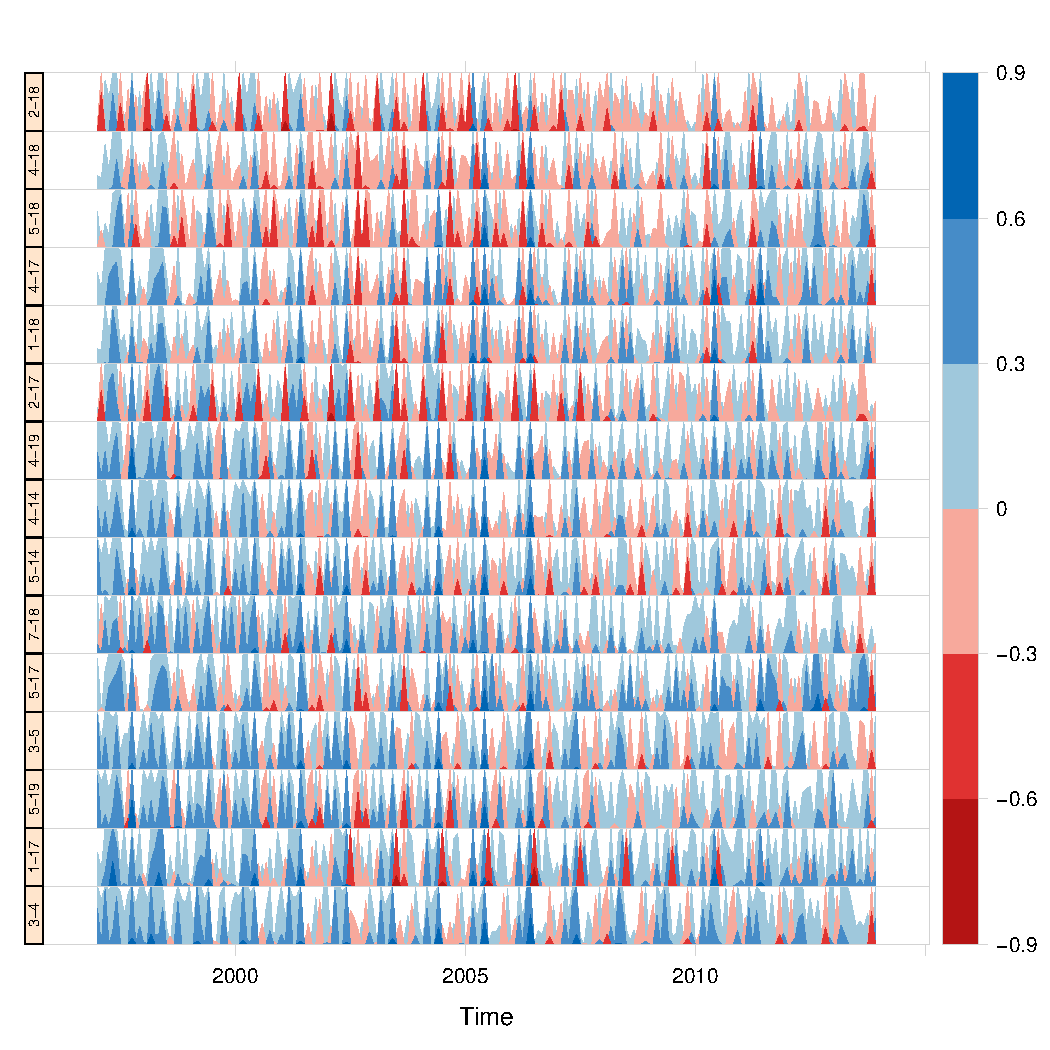
\includegraphics[scale=0.6]{figs/capitulo5/horizonplot_series_rad2}
% \caption{Correlation coefficient of solar irradiation at the horizontal plane: evolution of a 15-year moving window of monthly values, for the 15 cluster pairs showing the smallest median correlation values. Monthly negative correlations (in red) and monthly positive correlations (in blue) are represented in the same axis to facilitate the comparison of the multiple time-series. Also, higher correlation values overlap with lower ones, enabling a compact presentation of all the information in a narrower plot. The cluster pairs are indicated on the left, while the year in the x-axis indicates the end of each 15-year moving window.}
% \label{horizonplot_rad}
% \end{figure}

% The most relevant pairs in terms of complementarity include a northern (1, 2, 4 or 5) and a south-eastern cluster (17 or 18), as can be seen in figure \ref{horizonplot_rad}. The negative correlations for these pairs reach values below -0.6, at least in some 15-year sub-periods. These clusters are negatively correlated in most cases. Clusters 19 and 14 (southern and south-western IP) are also negative correlated with clusters in the north, although with lower values than the south-eastern clusters.

% It is important to notice the appearance of cluster pairs 3-4 and 3-5 in this figure. These clusters are closer than the previously commented cases, which highlights the adequacy of the clustering method. All three are Atlantic coast clusters, but while cluster 3 includes part of the western coast, clusters 4 and 5 are northern coast areas. This fact, together with the position of the main mountain ranges, can explain their partially complementary behaviour.

% %It is important to notice the appearance of cluster pairs 3-4 and 3-5 in this figure. These clusters are closer than the previously commented cases.  All three are Atlantic coast clusters, but while cluster 3 includes part of the western coast, clusters 4 and 5 are northern coast areas. This fact, together with the position of the main mountain ranges, can explain their partially complementary behavior. On the other hand, the 15-year moving window reveals interesting changes with time for all the cluster pairs, as there are higher and more frequent negative correlations in the middle 15-year sub-periods (those ending around 2005). 

% In order to highlight the months with maximum anti-correlation,  figure \ref{horizonplot_months_rad} presents, for the same 15 cluster pairs as above, the minimum values of the monthly correlation coefficient (where the minimum for each month is calculated over all 15-year sub-periods). Differences between months are clearly observed in this graph. Only two months (March and June) show consistently positive values of this parameter, and therefore a low complementarity. In the other months, this parameter has predominantly negative values, revealing a certain degree of complementarity. July, August and September show rather low values and relatively high complementarity, which is important as these are months with a high productivity and also include the summer demand peak. In general,  for the second half of the year, the values of this minimum correlation value are lower than for the first half of the year.

% \begin{figure}[h!]
% 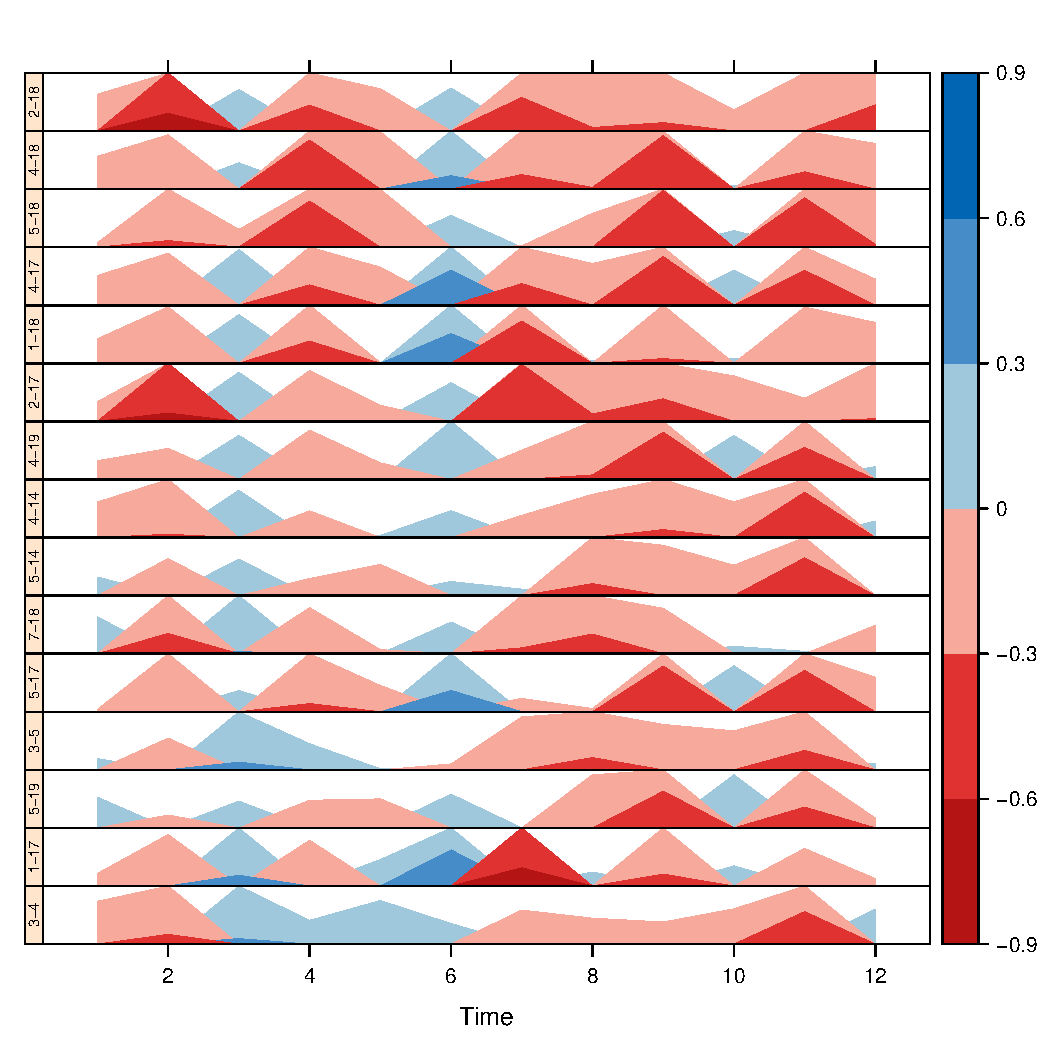
\includegraphics[scale=0.6]{figs/capitulo5/horizonplot_months_rad2}
% \caption{Correlation coefficient of solar irradiation at the horizontal plane: minimum values of the monthly correlation coefficient, for the same cluster pairs as figure \ref{horizonplot_rad}. The minimum is calculated over all 15-year sub-periods. The type of representation of correlation values is the same as in figure \ref{horizonplot_rad}. The cluster pairs are indicated on the left, while the numbers in the x-axis indicate the months.}
% \label{horizonplot_months_rad}
% \end{figure}

\section{Conclusion}
A detailed understanding of the space-time variability characteristics of renewable energies is fundamental for an adequate planning and management of the electrical system. In this chapter, a multi-step scheme to analyze spatial and temporal variability of renewable resources and production is described, which is implemented here for solar irradiation and photovoltaic energy yield. The method is comprehensive, as it includes 4 different steps covering spatial and temporal variability, spatial complementarity and also a detailed calculation of PV yield that is not usually taken into account in other studies of this subject. The 4 steps are:
\begin{enumerate}
\item Regionalization by an objective clustering procedure, that facilitates the inter-comparison between sub-regions and the spatial analysis. 
\item Assessment of energy yield considering different tracking systems, with a model that includes a large number of processes affecting the final power output.
\item Quantification of temporal variability in different time-scales with a robust metric, the coefficient of variation (CV). Due to its dimensionless character, this metric allows for a direct intercomparison of different magnitudes and energy resources.
\item Spatial complementarity assessment using the correlation coefficient, revealing potential options for smoothing out resource and production variability.
\end{enumerate}

The procedure is implemented over the Iberian Peninsula as an example of the scheme applicability. This region has been selected due to its large variety of climates and relevant electricity network characteristics, as it is internally well interconnected but externally it is poorly integrated with other electrical systems. A 30-year period of satellite data has been applied to analyze variability by subregions. An interannual time scale is selected for the variability analysis, due to its importance for the reliability and the financial viability of renewable energy production. A stable year-to-year production also contributes to reducing year-to-year price oscillations. Relationships between subregions of the IP are investigated in order to assess complementarity and detect possible compensation options. The procedure is applied to solar resource (global horizontal irradiation) and also to the PV yield with different tracking systems.

A fundamental contribution of the present study is the consideration of tilted panels and the quantification of differences between tracking systems. It has been proved that this kind of assessment is relevant in the variability analysis. In particular, we show that the increase in PV yield when passing from fixed tilted PV panels to one-axis tracking panels is non-linear, and depends strongly on the value of fixed panel energy yield: subregions with a larger fixed panel productivity show a larger relative increase with the use of a one-axis tracking system. In contrast, the PV yield increase between one-axis and two-axes systems is almost linear.

The clustering method has proved its selective character for detecting sub-regions with relevant differences in solar resource as it is shown in the case of study. This is illustrated, for instance, in the selection of cluster pairs formed by two Atlantic coast subregions as pairs showing a relatively high complementarity. It has been also shown that a moving window is useful to detect sub-periods of higher correlation between regions. The correlation characteristics of cluster pairs change over time if shorter 15-year sub-periods are considered, instead of the whole 30-year period of data. Negative correlation values are detected for most months, with two exceptions: March and June. July, August and September show relatively high anticorrelation between certain clusters, which is important as these months include the summer demand peak. 

This work provides a robust and comprehensive methodology that can be extended to other domains and to other timescales. The method can also be adapted to other types of renewable energy generation, like wind or solar thermoelectric, and can also provide combined assessments of different renewable resources, offering for example information about complementarity of solar and wind energy. Future applications of the method will explore such extensions.

% A detailed understanding of the space-time variability characteristics of renewable energies is fundamental for an adequate planning and management of the electrical system. In this paper, a multi-step scheme to analyze spatial and temporal variability of renewable resources and production is described, which is implemented here for solar irradiation and photovoltaic energy yield. The method is comprehensive, as it includes 4 different steps covering spatial and temporal variability, spatial complementarity and also a detailed calculation of PV yieldthat usually is not taken into account in other studies of this subject. The 4 steps are:
% \begin{enumerate}
% \item Regionalization by an objective clustering procedure, that facilitates the inter-comparison between sub-regions and the spatial analysis. 
% \item Assessment of energy yield considering different tracking systems, with a model that includes a large number of processes affecting the final power output.
% \item Quantification of temporal variability in different time-scales with a robust metric, the coefficient of variation (CV). Due to its dimensionless character, this metric allows for a direct intercomparison of different magnitudes and energy resources.
% \item Spatial complementarity assessment using the correlation coefficient, revealing potential options for smoothing out resource and production variability.
% \end{enumerate}

% The procedure is implemented over the Iberian Peninsula as an example of the scheme applicability. This region has been selected due to its large variety of climates and relevant electricity network characteristics, as it is internally well interconnected but externally it is poorly integrated with other electrical systems. A 30-year period of satellite data has been employed to analyze variability by subregions. An interannual time scale is selected for the variability analysis, due to its importance for the reliability and the financial viability of renewable energy production. A stable year-to-year production also contributes to reducing year-to-year price oscillations. Relationships between subregions of the IP are investigated in order to assess complementarity and detect possible compensation options. The procedure is applied to solar resource (global horizontal irradiation) and also to the PV yield with different tracking systems.

% A fundamental contribution of the present study is the consideration of tilted panels and the quantification of differences between tracking systems. It has been proved that this kind of assessment is relevant in the variability analysis. In particular, we show that the increase in PV yield when passing from fixed tilted PV panels to one-axis tracking panels is non-linear, and depends strongly on the value of fixed panel energy yield: subregions with a larger fixed panel productivity show a larger relative increase with the use of a one-axis tracking system. In contrast, the PV yield increase between one-axis and two-axes systems is almost linear.

% %It is shown that solar irradiation is a particularly reliable resource over the region. Interannual variability of solar irradiation is small in comparison to other renewable energy sources. Variability of the productivity is higher than that of the solar irradiation, and increases with the complexity of the tracking system. But this increase in variability of the different PV generation methods is rather limited, and the year-to-year productivity remains stable. For example, the most variable production method (two-axis panel) shows an interannual CV of the yearly productivity between 3 and 5 percent, for most of the subregions. It is also noteworthy that a higher increase in productivity is not associated to a higher increase in variability when more complex tracking systems are used. The annual cycle of variability shows interesting results, as in summer the interannual variability of solar resource is very similar to the variability of the PV panel productivities, while important differences are found in winter. A remarkable result is that the variability of fixed tilted panels in summer is even lower that the variability of solar irradiation at the horizontal plane.

% The clustering method has proved its selective character for detecting sub-regions with relevant differences in solar resource as it is shown in the case of study. This is illustrated, for instance, in the selection of cluster pairs formed by two Atlantic coast subregions as pairs showing a relatively high complementarity. It has been shown also that a mobile window is useful to detect sub-periods of higher correlation between regions. The correlation characteristics of cluster pairs change over time if shorter 15-year sub-periods are considered, instead of the whole 30-year period of data. Negative correlation values are detected for most months, with two exceptions: March and June. July, August and September show relatively high anticorrelation between certain clusters, which is important as these months include the summer demand peak. 

% % This is illustrated by the north-eastern cluster corresponding to the central Ebro valley, which shows high PV productivity and very low variability, despite being located near the northern coast and Pyrenees clusters that show very different characteristics.

% %Another example is the selection of cluster pairs formed by two Atlantic coast subregions as pairs showing a relatively high complementarity. On the other hand, the complementarity analysis shows that the correlation characteristics of cluster pairs change over time if shorter 15-year sub-periods are considered, instead of the whole 30-year period of data. Negative correlation values are detected for most months, with two exceptions: March and June. July, August and September show relatively high anticorrelation between certain clusters, which is important as these months include the summer demand peak. 

% This work provides a robust and comprehensive methodology that can be extended to other domains and to other timescales. The method can also be adapted to other types of renewable energy generation, like wind or solar thermoelectric, and can also provide combined assessments of different renewable resources, offering for example information about complementarity of solar and wind energy. Future applications of the method will explore such extensions.

% \begin{subappendices}

% \section{Appendix}
  
% \subsection{Yearly mean values and variability}

\section*{Appendix A}
\subsection*{Yearly mean values and variability}

The highest values of CV for solar irradiation (above $4\%$) are seen in clusters 8, 4 and 5. These clusters correspond to the Pyrenees and the northern Cantabric coast. This behavior can be explained in part through the influence of variable summer cloudiness, as these areas are not affected by the summer dryness typical of the Mediterranean climate of most of the Iberian Peninsula. Southern and Central regions are the least variable. Remarkably, the lowest value of CV is found in cluster 11, corresponding to the central Ebro basin, located at the north of the Iberian Peninsula. Very low values near $2\%$   are also found in the southwestern clusters (4 and 19), a result that coincides with \cite{Gil2015}. Finally, the northwestern clusters (2 and 7) show a higher value than the northeastern cluster (13), despite sharing the same latitude. The northwestern clusters are particularly influenced by the Azores high position and interannual variability.

Irradiation data and their CV are also graphically represented in Figure \ref{SolarIrradiation_CV_maps}, showing their geographical distribution. The functions represented at the margins of the graphs, show respectively the latitudinal and longitudinally aggregated value of the variable. In latitude, both, global irradiation and CV are inversely related. Regarding the longitude axis, a contrast between coastal and interior values is seen for the irradiance, while the CV shows a complex behavior, predominantly with higher values near the western and eastern coast than in the interior parts.

\begin{figure}[!tbp]
  \centering
  \subfloat[]{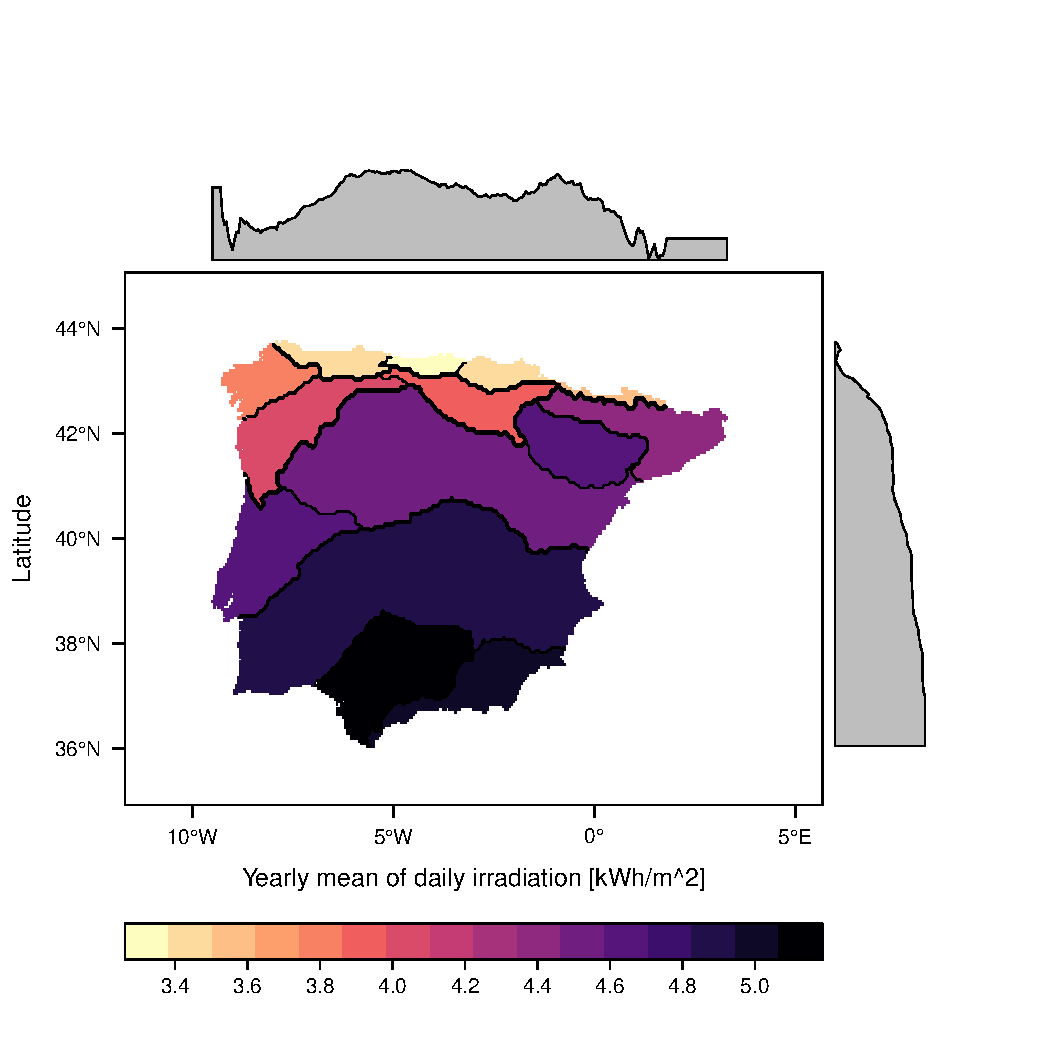
\includegraphics[width=0.45\textwidth]{figs/capitulo5/Solariradiationmap_yearly2.pdf}\label{fig:f1}}
  \hfill
  \subfloat[]{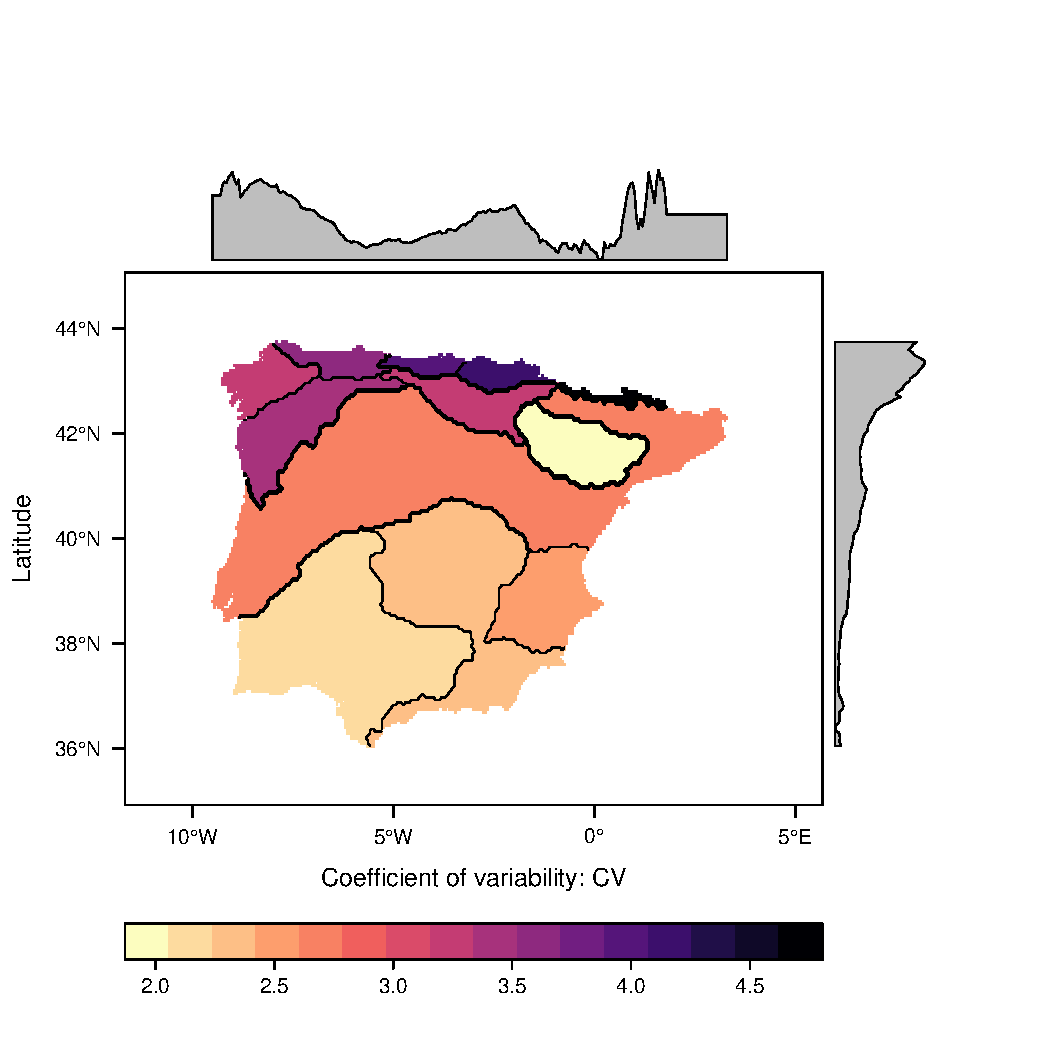
\includegraphics[width=0.45\textwidth]{figs/capitulo5/SolarirradiationCVmap_yearly2.pdf}\label{fig:f2}}
  \caption[Yearly mean of solar irradiation and variability over the Iberian Peninsula]{Yearly mean of solar irradiation and its CV. Figure [a] shows the yearly mean of daily irradiation period 1983-2013 $\left[\si{\kilo\watthour\over\metro^2}\right]$. Figure [b] shows the coefficient of variability, CV of the yearly mean of daily irradiation}
\label{SolarIrradiation_CV_maps}
\end{figure}

Figure \ref{fig:mapsPVyCV} shows photovoltaic energy yield by tracking system and their CV values. The increase in the CV with different tracking typologies can be seen. In each case it is possible to appreciate the difference between northern Iberian Peninsula, with higher variability, and the southern Iberian Peninsula, with lower variability. An exception to this latitudinal dependence is again the central Ebro basin, which stands out as the cluster with the lowest variability, particularly for the two-axes tracking. There are also differences between the western and eastern sides of the Iberian Peninsula, showing the last one lower variability on this time scale. 

\begin{figure}[!tbp]
\centering
\subfloat[]{
  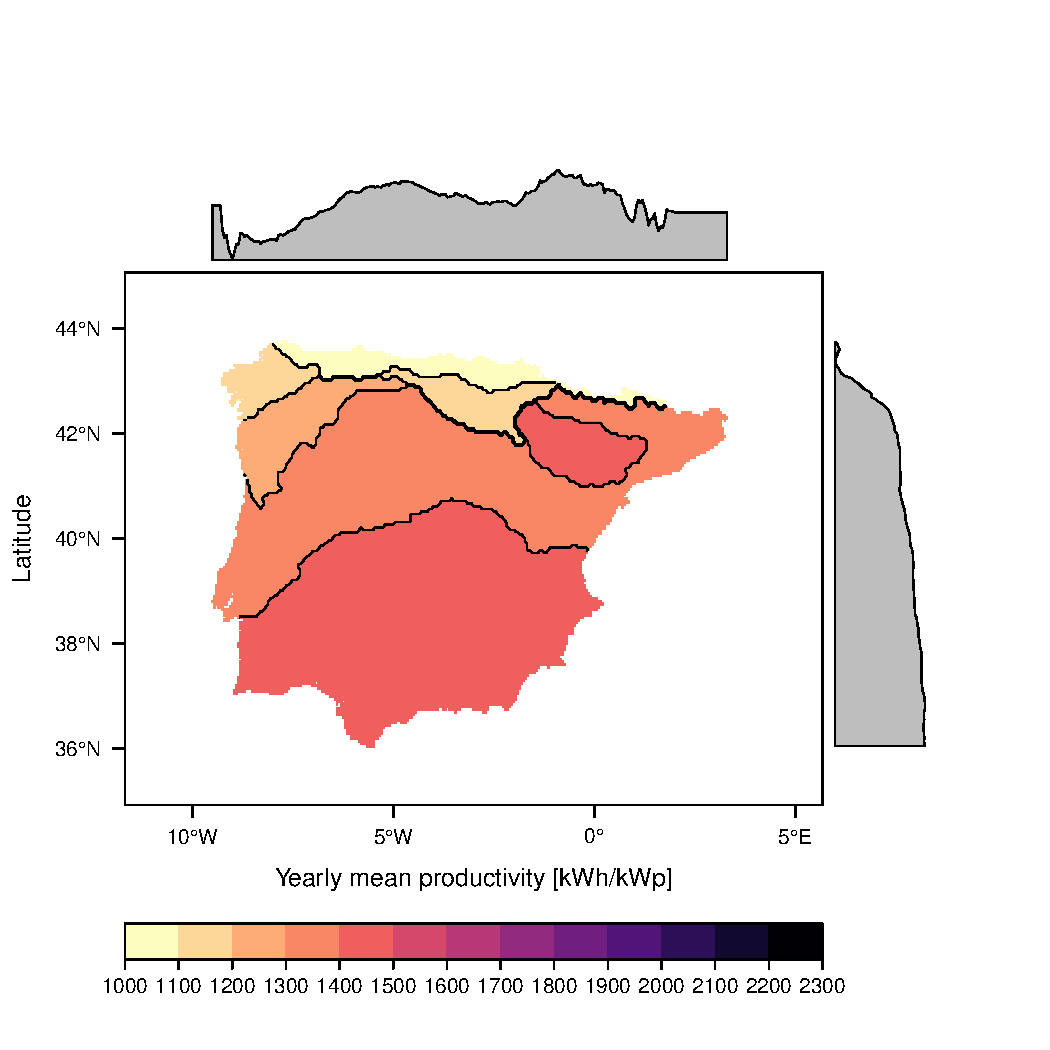
\includegraphics[width=0.43\textwidth]{figs/capitulo5/ProductivityFixed_yearlymean3}
}
\subfloat[]{
  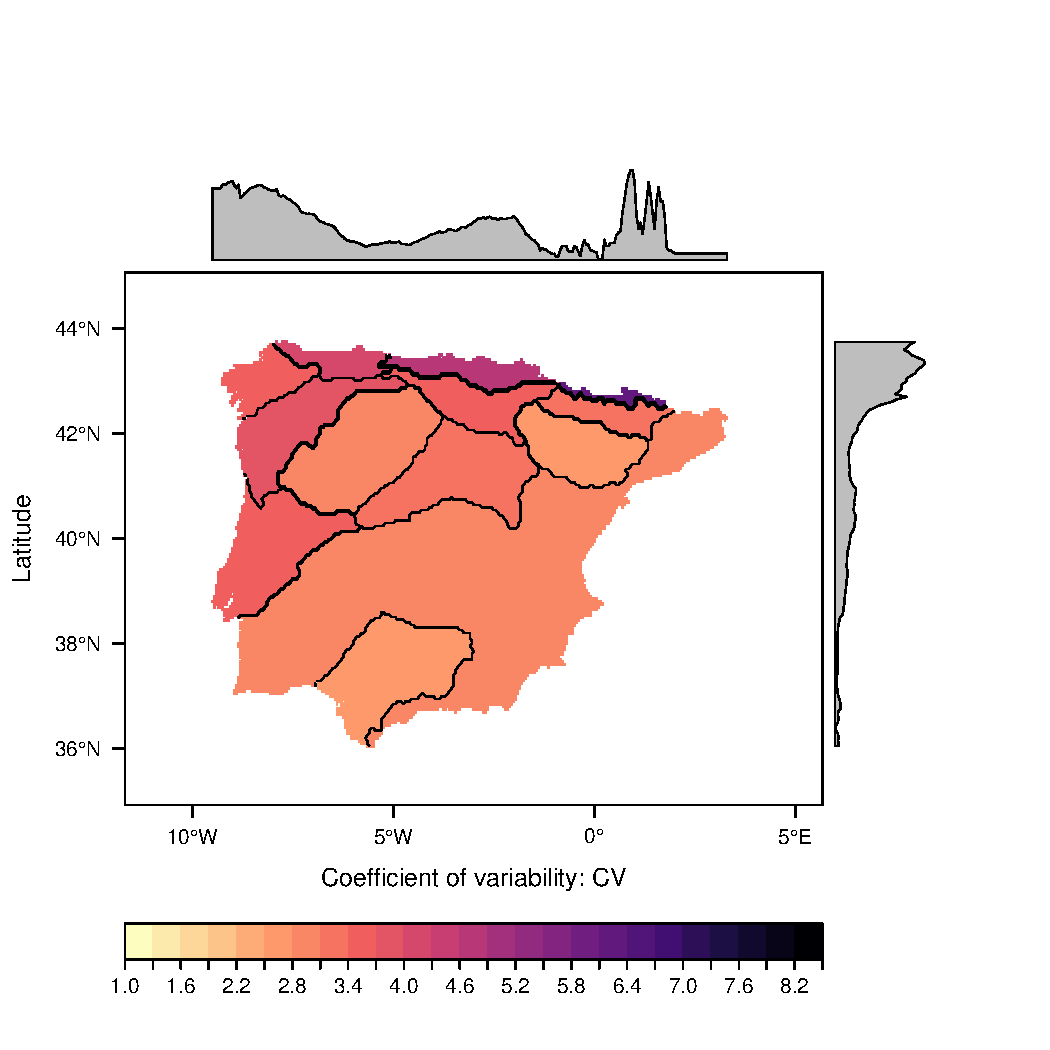
\includegraphics[width=0.43\textwidth]{figs/capitulo5/ProductivityCVfixed_yearlymean2}
}
\hspace{0mm}
\subfloat[]{
  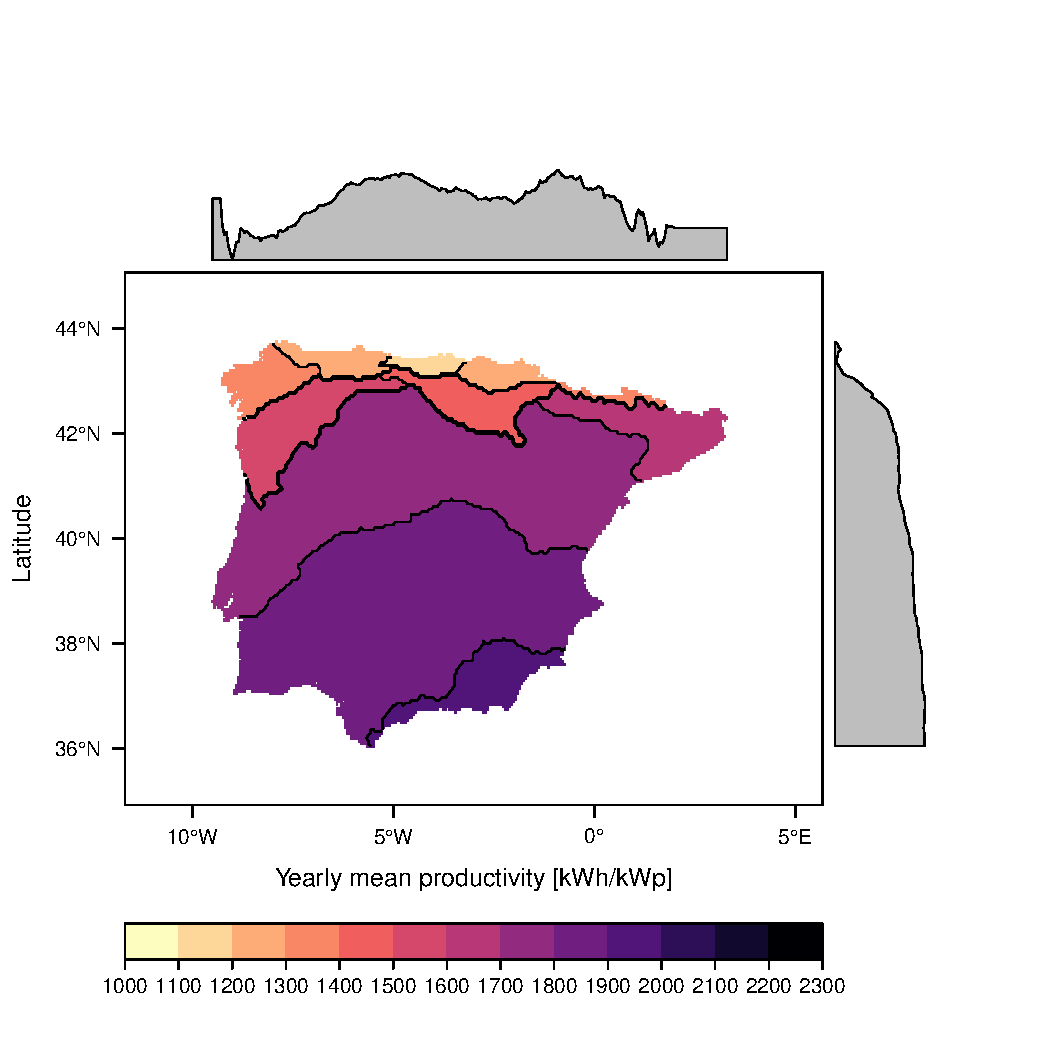
\includegraphics[width=0.43\textwidth]{figs/capitulo5/ProductivityHoriz_yearlymean3}
}
\subfloat[]{
  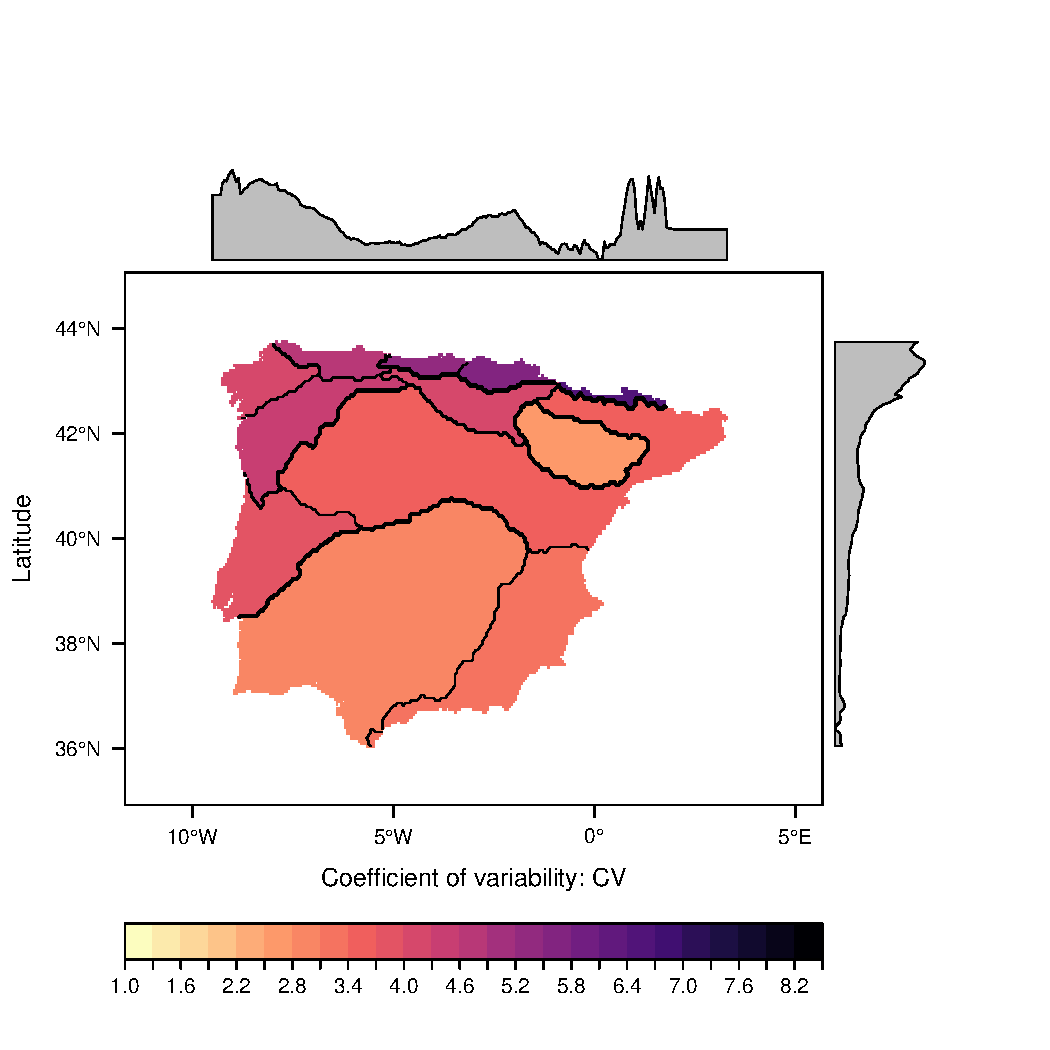
\includegraphics[width=0.43\textwidth]{figs/capitulo5/ProductivityCVHoriz_yearlymean2}
}
\hspace{0mm}
\subfloat[]{ 
  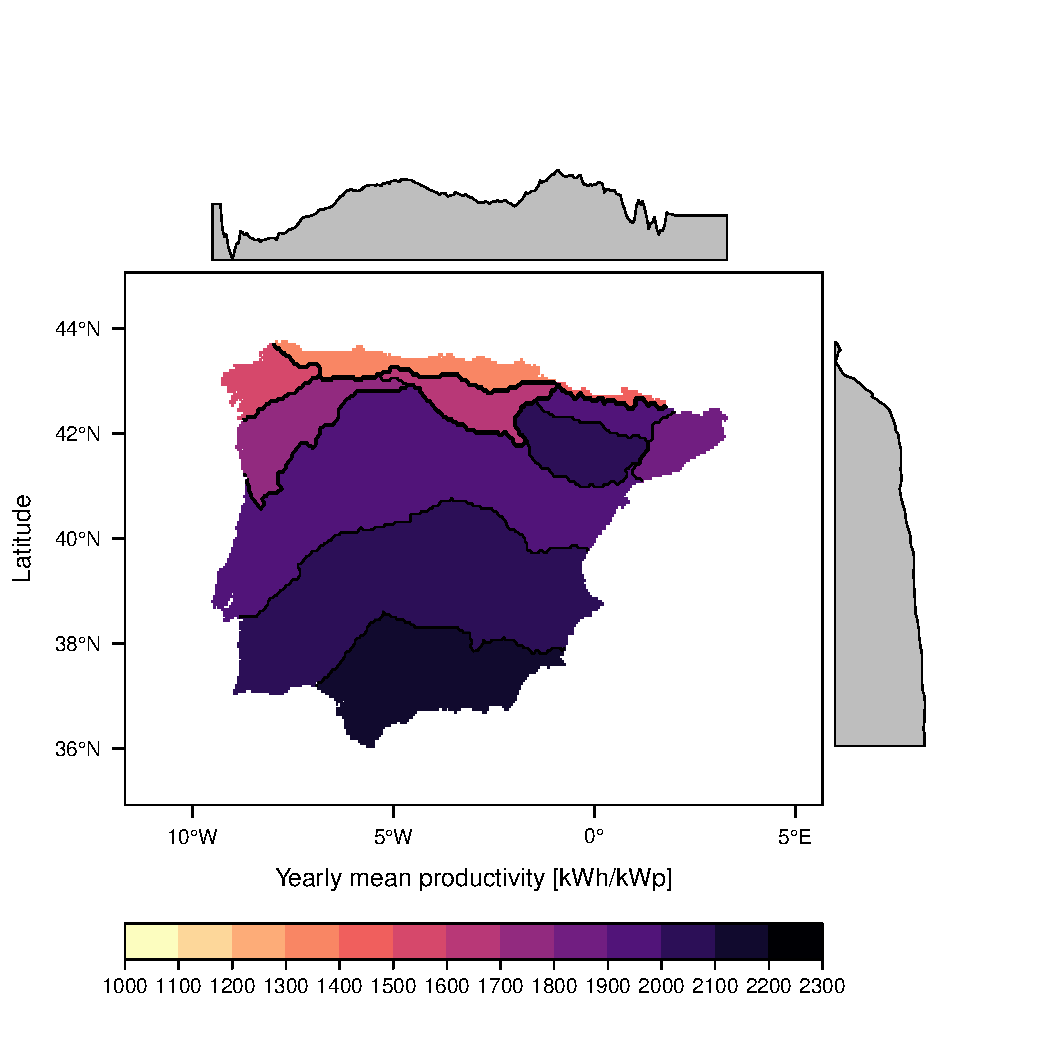
\includegraphics[width=0.43\textwidth]{figs/capitulo5/ProductivityTwo_yearlymean3}
}
\subfloat[]{
  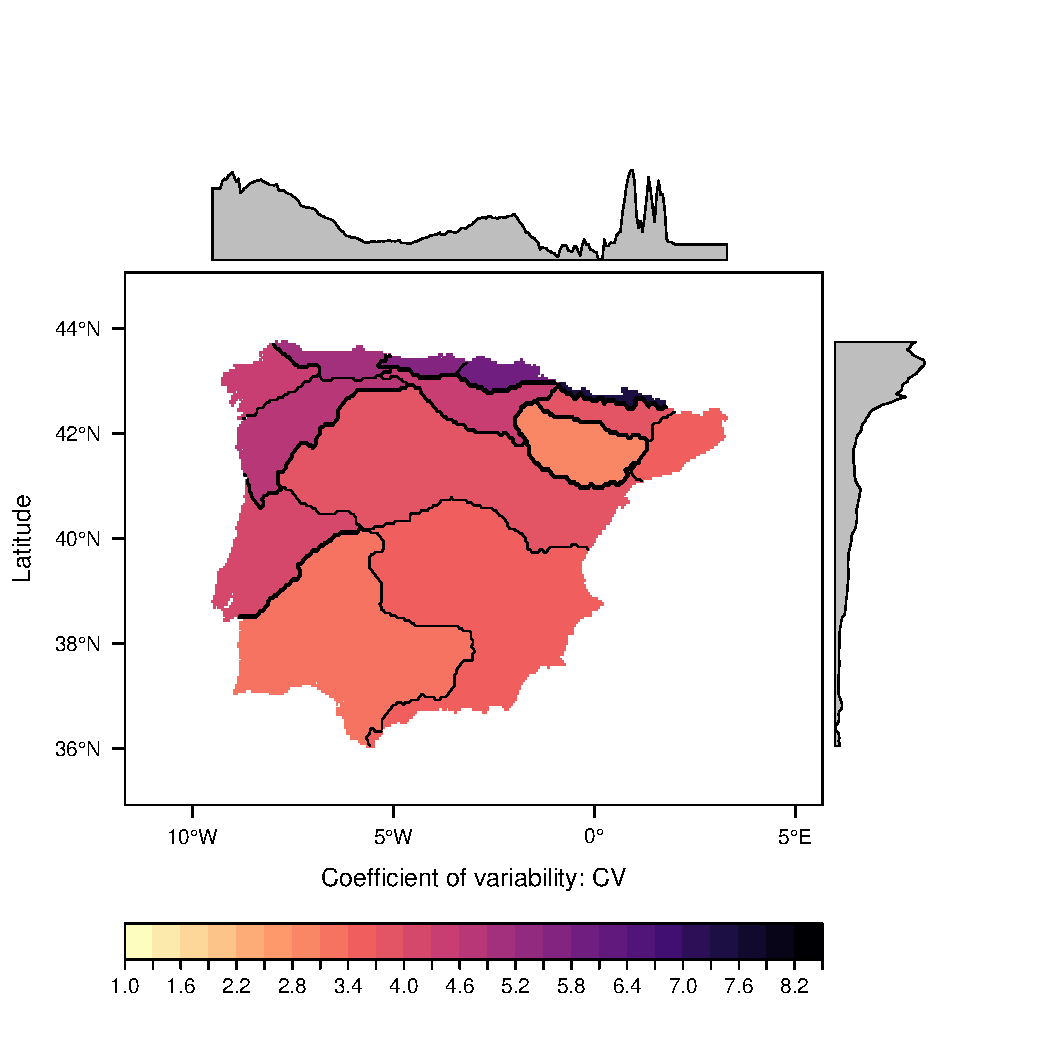
\includegraphics[width=0.43\textwidth]{figs/capitulo5/ProductivityCVTwo_yearlymean2}
}
\caption[Yearly mean yield and variability by tracking type and cluster over the Iberian Peninsula]{First column: maps of yearly mean yield by tracking type $\left[\si{\kilo\watthour\per\kilo\wattpeak}\right]$, mean by cluster (a, fixed; c, 'ona axis'; e, 'two axes'). Second column: maps of interannual coefficient of variability, CV, of the yearly mean yield by tracking type and by cluster (b, 'fixed'; d 'one axis'; f, 'two axes')}
\label{fig:mapsPVyCV}
\end{figure}

Figure \ref{yearly_productivity_and_CV} shows differences between clusters and tracking typologies combining CV and yield in the same graph. Straight lines are representing mean values for the whole IP. The CV values for yearly yield are around $4\%$ for the two-axes tracking system in the whole area, and close to $3\%$ for the fixed panels. The CV of the annual mean of daily irradiation is about $2.3\%$.  For the x axis, where yield is represented, areas with higher resource have higher PV yield and differences between clusters are larger for those areas. It is easy to notice that by comparing clusters 1 and 19.

This figure also facilitates visualization of each cluster's size, due to the fact that each point represents one cell of the domain, and reveals the compactness of most clusters. Only a couple of clusters (8 and 18) show wide dispersion of individual points. Cluster 8 includes the highest mountains of the IP, which could explain this dispersion. For cluster 18, it is seen that although the majority of its points have values of CV below the mean of the IP, there are some of them with high values of CV. 

\begin{figure}[!tbp]
  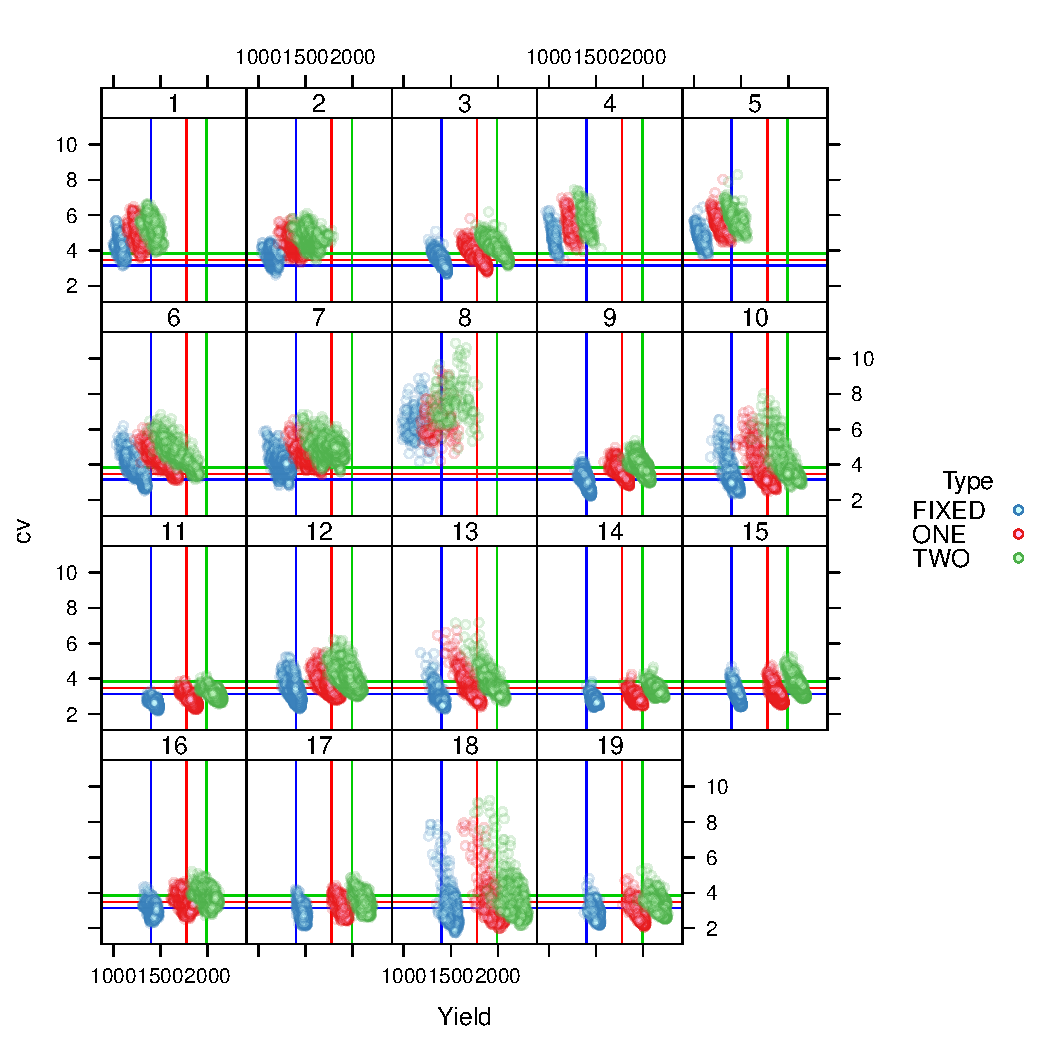
\includegraphics[width=\textwidth]{figs/capitulo5/cv_productivity4NEW.pdf}
  \caption[Yearly mean of solar irradiation and variability by tracking type and cluster for each cell over the Iberian Peninsula]{Yearly mean of PV yield $\left[\si{\kilo\watthour\per\kilo\wattpeak}\right]$ (horizontal axis) and CV (vertical axis in percentage) by cluster and tracking system. The individual points correspond to individual grid points forming part of the clusters. Transparency of dots is applied to show importance of the number of points inside the clusters regarding its value of CV.}
  \label{yearly_productivity_and_CV}
\end{figure}

% The results for the CV of the yearly mean of daily irradiation and of the annual mean yield by tracking type, aggregated by cluster, are shown in table \ref{tabla2}. Also, yearly mean of daily irradiation is represented, showing differences in resource among areas, as well as yield differences.

% \begin{center}
% \begin{table}
% \begin{tabular}[0.7\textwidth]{c|c|c|c|c|c|c|c|c}
% Zone & $G(0)$ $[\si{\kilo\watthour\over\metro^2}]$ & $CV_{G0}$ & $Y_{fixed}$ $[\si{\kilo\watthour\per\kilo\wattpeak}]$ & $CV_{fixed}$ & $Y_{one}$ $[\si{\kilo\watthour\per\kilo\wattpeak}]$ & $CV_{one}$ & $Y_{two}$ $[\si{\kilo\watthour\per\kilo\wattpeak}]$ & $CV_{two}$\\
% \hline
% 1 & 3.4 & 3.6 & 1047 & 4.2 & 1225 & 4.9 & 1381 & 5.1\\ 
% 2 & 3.8 & 3.2 & 1120 & 3.6 & 1359 & 4.3 & 1520 & 4.6\\
% 3 & 4.6 & 2.8 & 1350 & 3.4 & 1720 & 3.7 & 1921 & 4.1\\
% 4 & 3.4 & 4.1 & 1024 & 4.7 & 1198 & 5.4 & 1351 & 5.7\\
% 5 & 3.4 & 4.2 & 1035 & 4.7 & 1226 & 5.5 & 1374 & 5.8\\
% 6 & 4.0 & 3.2 & 1190 & 3.7 & 1465 & 4.2 & 1640 & 4.5\\
% 7 & 4.1 & 3.4 & 1224 & 3.9 & 1530 & 4.4 & 1712 & 4.8\\
% 8 & 3.6 & 4.6 & 1099 & 6.3 & 1322 & 6.4 & 1473 & 7.5\\
% 9 & 4.5 & 2.7 & 1356 & 3.0 & 1725 & 3.5 & 1934 & 3.8\\
% 10 & 4.4 & 2.7 & 1367 & 3.2 & 1696 & 3.6 & 1937 & 3.9\\
% 11 & 4.7 & 2.0 & 1404 & 2.6 & 1787 & 2.7 & 2024 & 3.1\\
% 12 & 4.5 & 2.6 & 1348 & 3.1 & 1701 & 3.5 & 1911 & 3.8\\
% 13 & 4.4 & 2.7 & 1340 & 2.9 & 1660 & 3.4 & 1893 & 3.7\\
% 14 & 4.9 & 2.2 & 1423 & 2.8 & 1837 & 3.0 & 2047 & 3.4\\
% 15 & 4.9 & 2.3 & 1427 & 2.9 & 1837 & 3.0 & 2057 & 3.4\\
% 16 & 4.5 & 2.6 & 1374 & 3.0 & 1722 & 3.4 & 1946 & 3.7\\
% 17 & 4.9 & 2.5 & 1429 & 2.9 & 1830 & 3.3 & 2052 & 3.6\\
% 18 & 5.1 & 2.4 & 1470 & 2.9 & 1906 & 3.2 & 2123 & 3.5\\
% 19 & 5.1 & 2.1 & 1456 & 2.8 & 1891 & 2.8 & 2105 & 3.7\\
% \end{tabular}
% \caption{Values of yearly mean of daily irradiation, yearly yield by tracking system and interannual CV of yearly mean.}
% \label{tabla2}
% \end{table}
% \end{center}

% The highest values of global solar irradiation are found in clusters 14, 15, 17, 18, 19, which correspond to the south of the Iberian Peninsula. Besides this latitude-related maximum irradiation, a particularly high value of solar irradiation is found in cluster 11, clearly above all surrounding clusters in the northern half of the Iberian Peninsula. This cluster corresponds to the central Ebro basin, which is characterized by a very dry continental climate. It is a deep depression totally surrounded by mountain ranges like the Pyrenees,  which frequently cause a Föhn effect which reduces cloudiness and precipitation in comparison with other nearby clusters. Excluding this cluster, irradiation in the northern half of the Iberian Peninsula is lower than in the southern half, and the minimum values are found in clusters in the northern coast and the Pyrenees. The maximum solar irradiation is 50 percent higher than the minimum, which reflects the large climatic differences between clusters.

% The highest values of CV (above $4\%$) are seen in clusters 8, 4 and 5. These clusters correspond to the Pyrenees and the northern Cantabric coast. This behavior can be explained in part through the influence of variable summer cloudiness, as these areas are not affected by the summer dryness typical of the Mediterranean climate of most of the Iberian Peninsula. Southern and Central regions are the least variable. Remarkably, the lowest value of CV is found in cluster 11, corresponding to the central Ebro basin, located at the north of the Iberian Peninsula. Very low values near $2\%$   are also found in the southwestern clusters (4 and 19), a result that coincides with \cite{Gil2015}. Finally, the northwestern clusters (2 and 7) show a higher value than the northeastern cluster (13), despite sharing the same latitude. The northwestern clusters are particularly influenced by the Azores high position and interannual variability.

% Irradiation data and their CV are also graphically represented in figure \ref{SolarIrradiation_CV_maps}, showing their geographical distribution. The functions represented at the margins of the graphs, show respectively the latitudinal and longitudinally aggregated value of the variable. In latitude, both, global irradiation and CV evolve linearly and are inversely related. Regarding the longitude axis, a contrast between coastal and interior values is seen for the irradiance, while the CV shows a complex behavior, predominantly with higher values near the western and eastern coast than in the interior parts.

% \begin{figure}[!tbp]
%   \centering
%   \subfloat[]{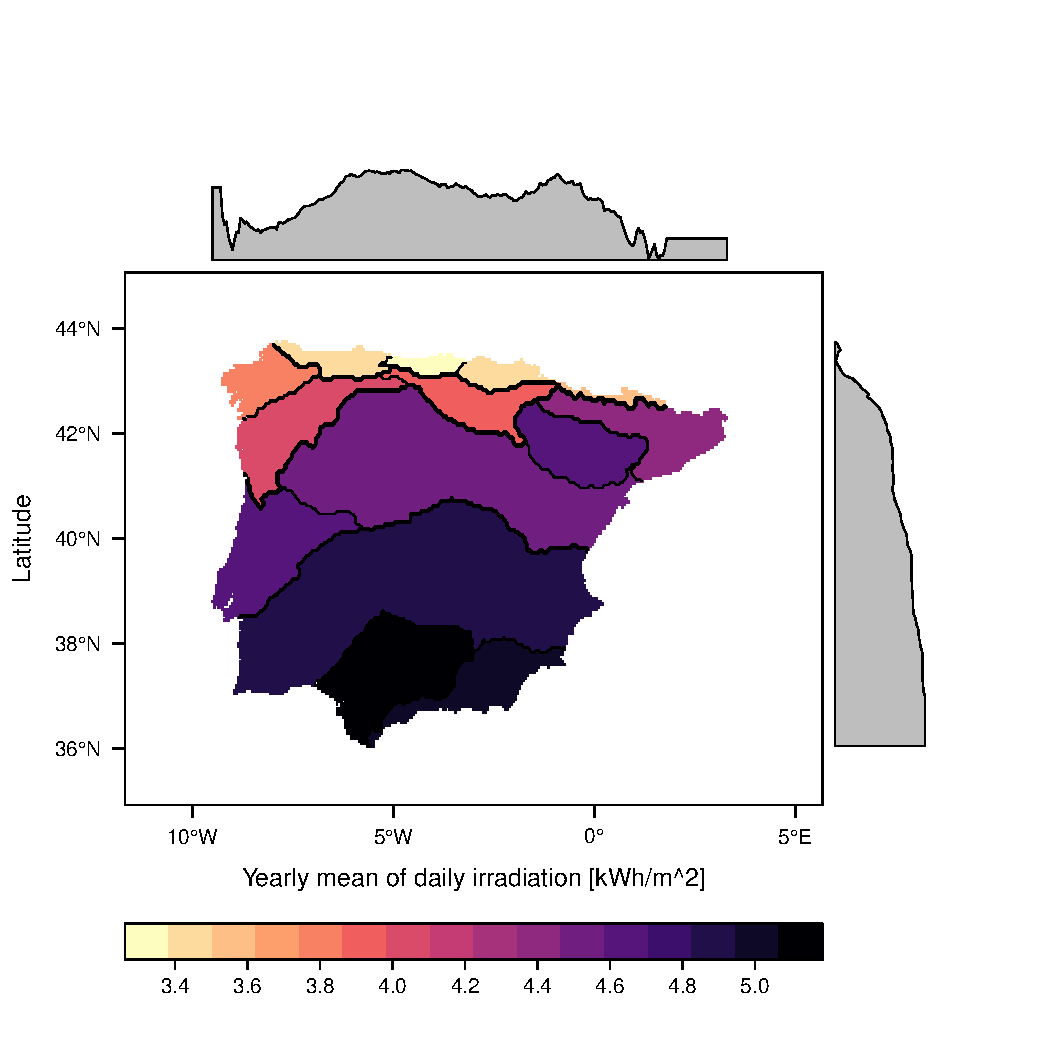
\includegraphics[width=0.45\textwidth]{figs/capitulo5/Solariradiationmap_yearly2.pdf}\label{fig:f1}}
%   \hfill
%   \subfloat[]{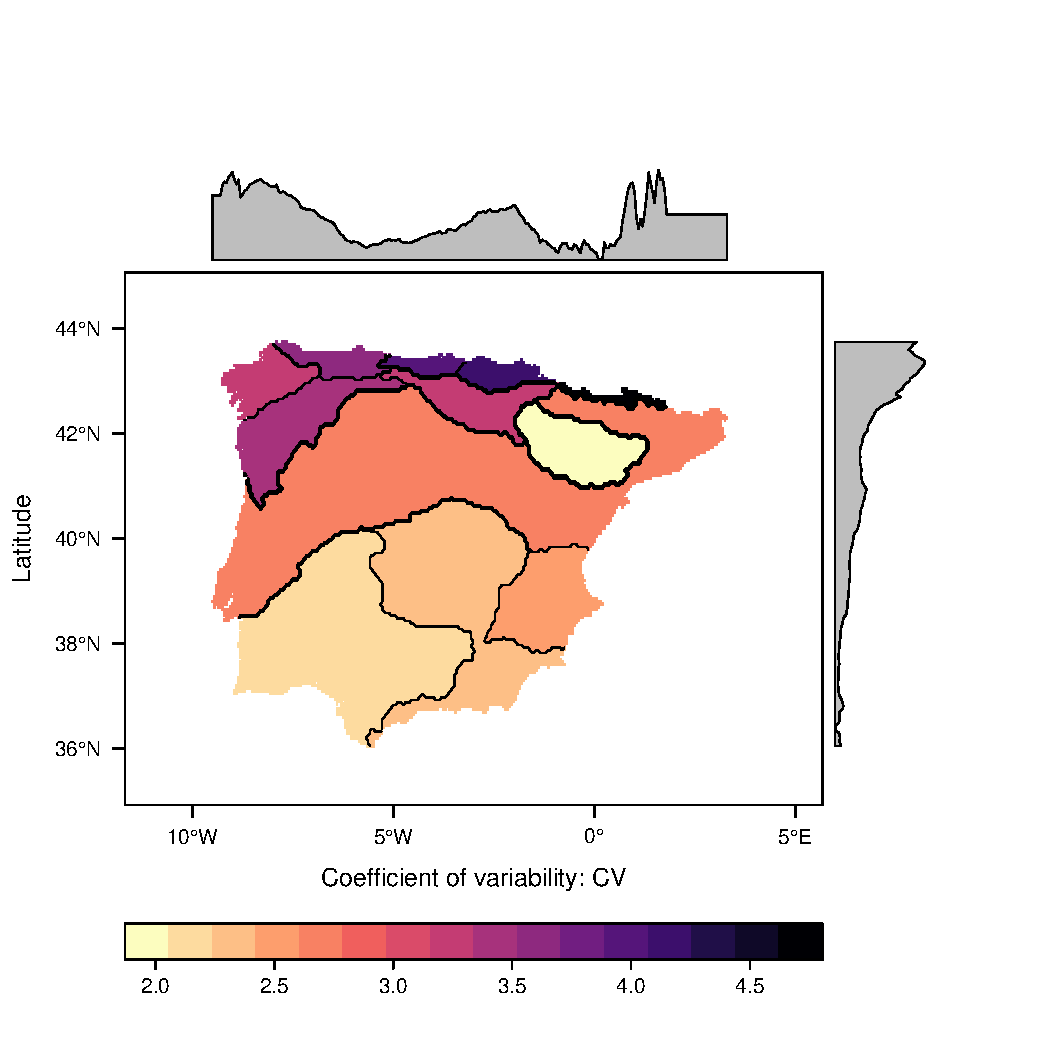
\includegraphics[width=0.45\textwidth]{figs/capitulo5/SolarirradiationCVmap_yearly2.pdf}\label{fig:f2}}
%   \caption{Solar irradiation yearly mean and  CV. Figure [a] shows the yearly mean of daily irradiation period 1983-2013 $[\si{\kilo\watthour\over\metro^2}]$. Figure [b] shows the coefficient of variability, CV of the yearly mean of daily irradiation}
% \label{SolarIrradiation_CV_maps}
% \end{figure}


% Figure \ref{mapas} shows CV values for solar irradiation on the horizontal plane and the photovoltaic energy yield by tracking system. This figure shows the increase in the CV from the irradiation on the horizontal plane to the different tracking typologies. In each case it is possible to appreciate the difference between northern Iberian Peninsula, with higher variability, and the southern Iberian Peninsula, with lower variability. An exception to this latitudinal dependence is again the central Ebro basin, which stands out as the cluster with the lowest variability, particularly for the two-axes tracking. There are also differences between the western and eastern sides of the Iberian Peninsula, showing the last one lower variability on this time scale. 

% \begin{figure}[!tbp]
% \centering
% \subfloat[]{
%   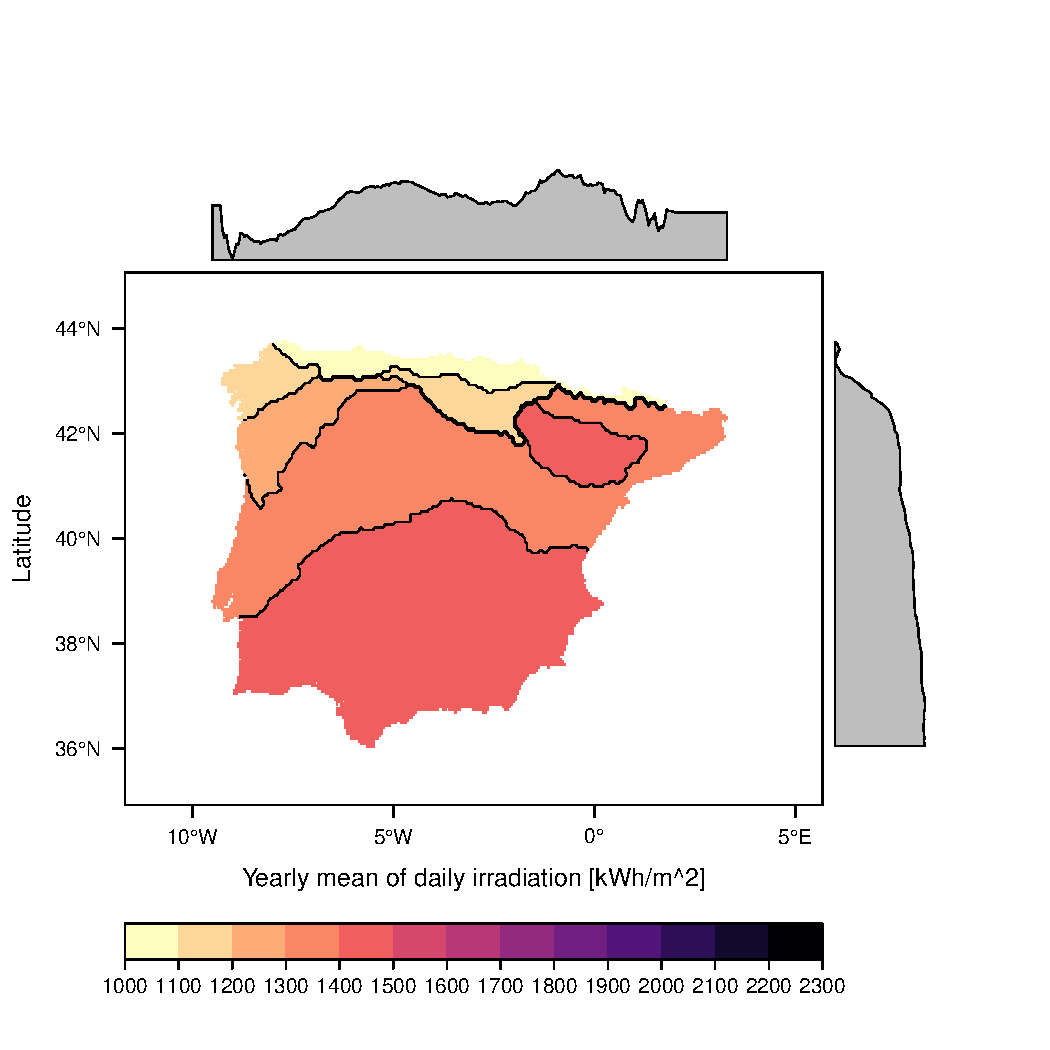
\includegraphics[width=0.43\textwidth]{figs/capitulo5/ProductivityFixed_yearlymean2}
% }
% \subfloat[]{
%   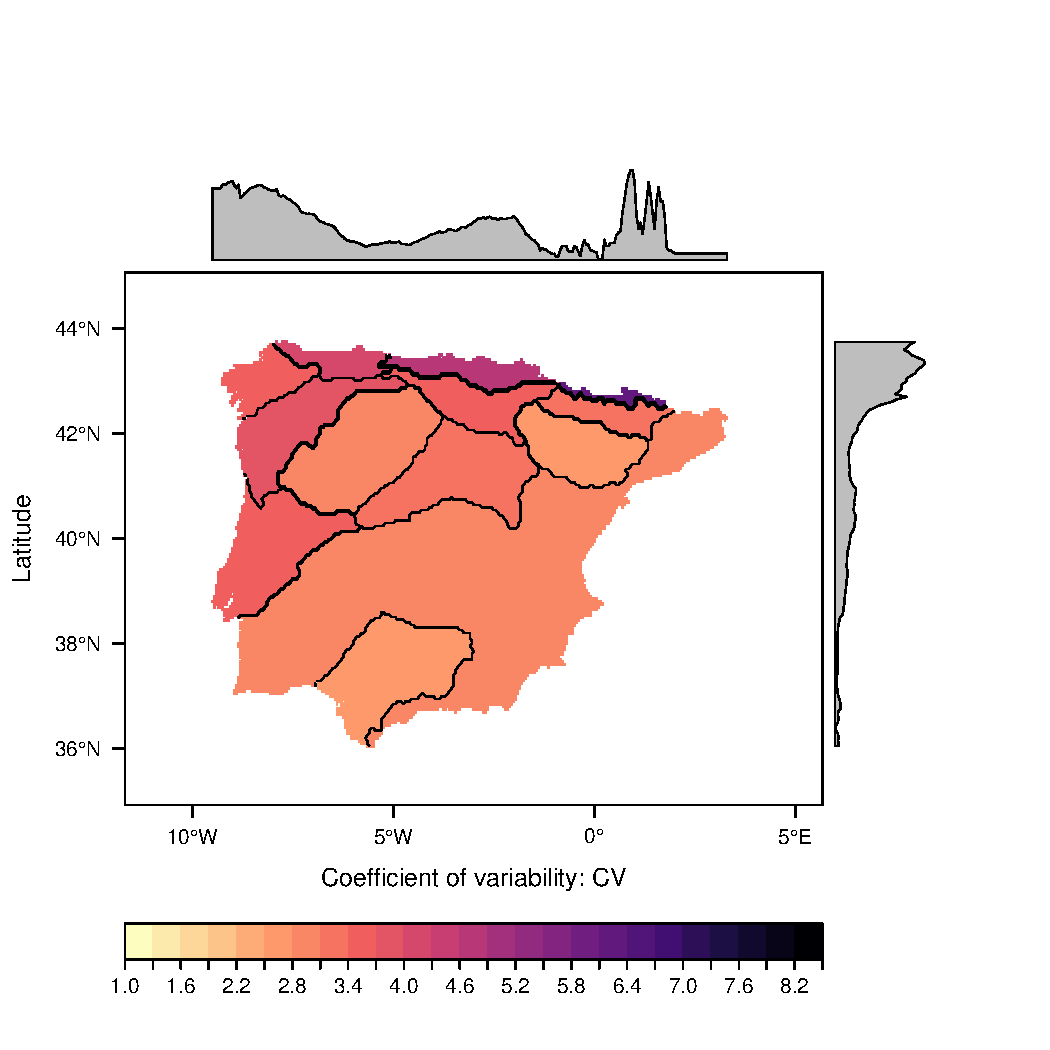
\includegraphics[width=0.43\textwidth]{figs/capitulo5/ProductivityCVfixed_yearlymean2}
% }
% \hspace{0mm}
% \subfloat[]{
%   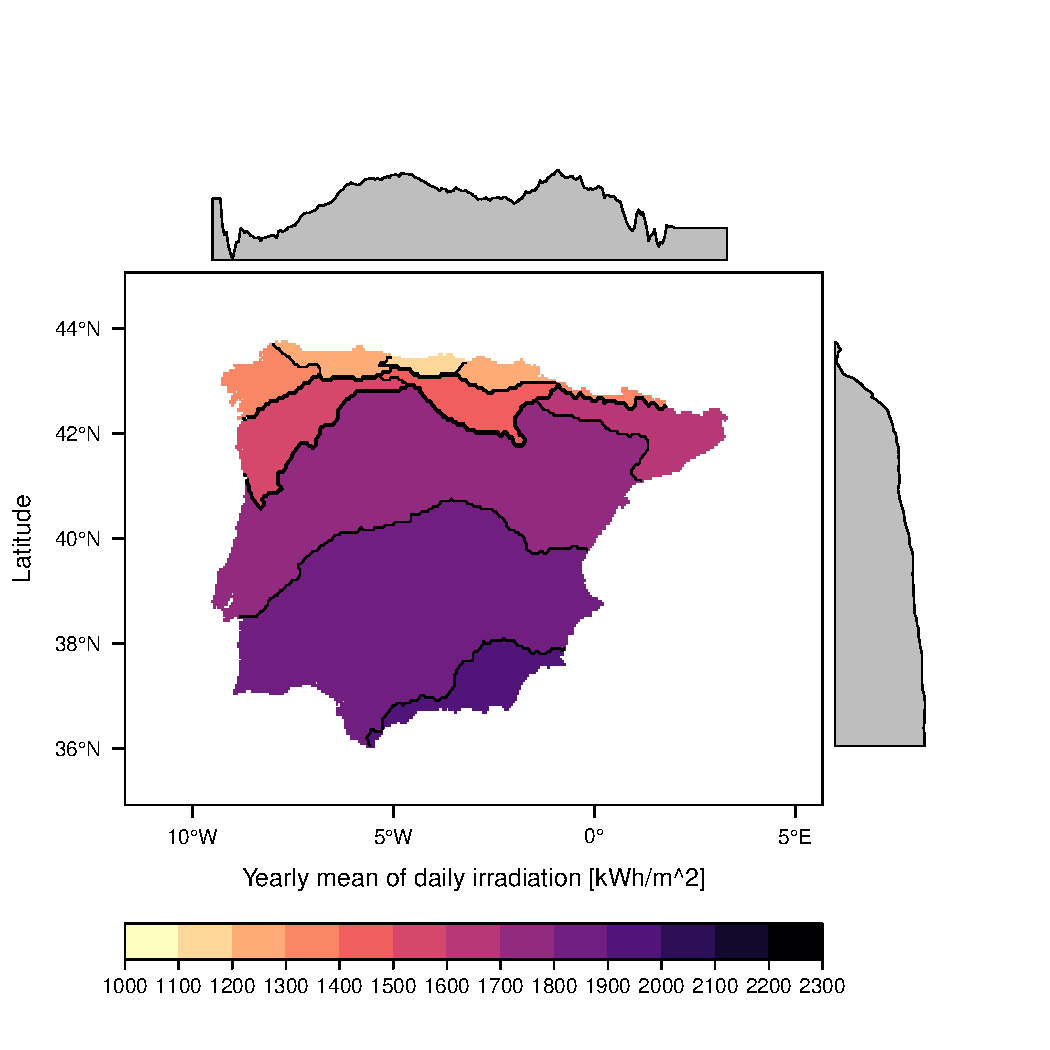
\includegraphics[width=0.43\textwidth]{figs/capitulo5/ProductivityHoriz_yearlymean2}
% }
% \subfloat[]{
%   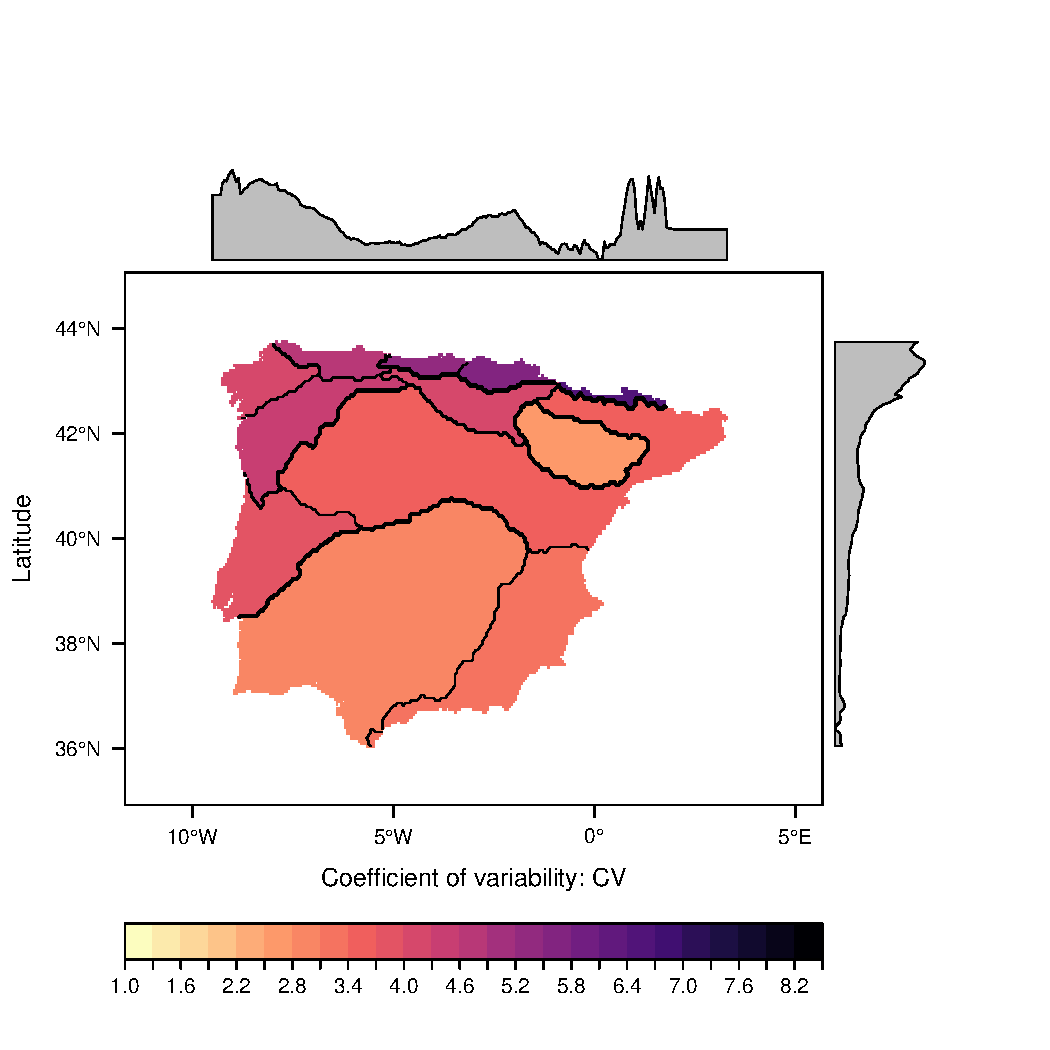
\includegraphics[width=0.43\textwidth]{figs/capitulo5/ProductivityCVHoriz_yearlymean2}
% }
% \hspace{0mm}
% \subfloat[]{ 
%   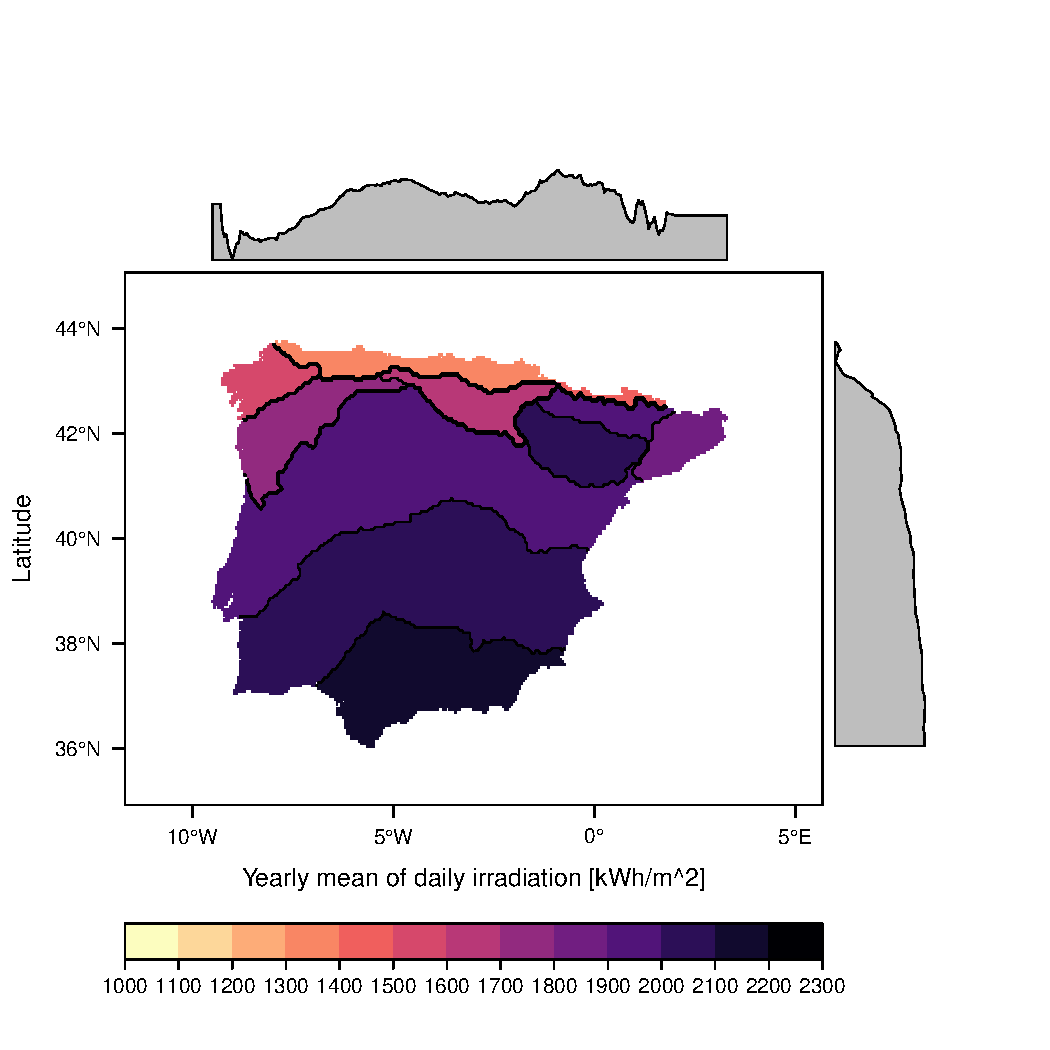
\includegraphics[width=0.43\textwidth]{figs/capitulo5/ProductivityTwo_yearlymean2}
% }
% \subfloat[]{
%   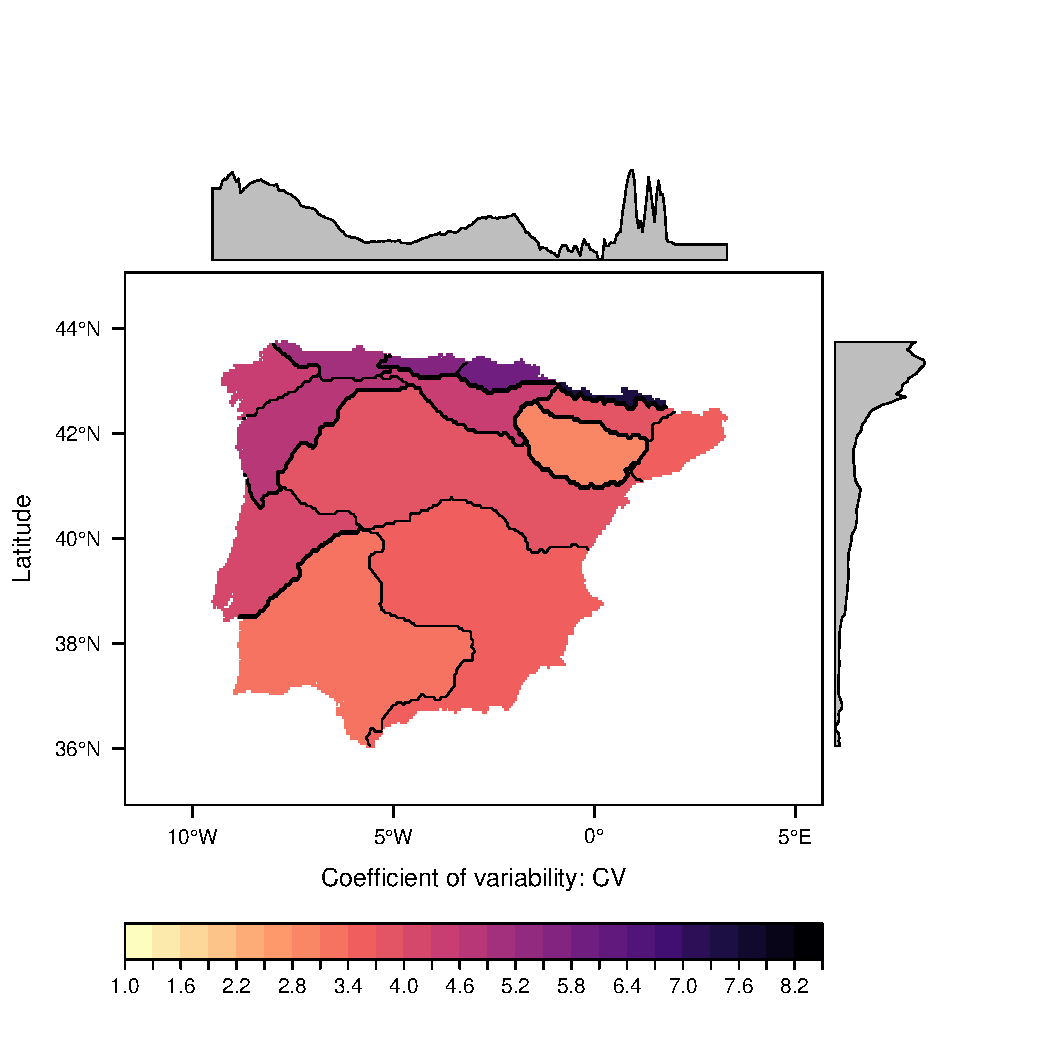
\includegraphics[width=0.43\textwidth]{figs/capitulo5/ProductivityCVTwo_yearlymean2}
% }
% \caption{First column: maps of yearly mean yield by tracking type $[\si{\kilo\watthour\per\kilo\wattpeak}]$, mean by cluster (a, fixed; c, '1 axis'; e, '2 axes'). Second column: maps of interannual coefficient of variability, CV, of the yearly mean yield by tracking type and by cluster (b, 'fixed'; d '1 axis'; f, '2 axes')}
% \label{mapas}
% \end{figure}

% Figure \ref{yearly_productivity_and_CV} shows differences between clusters and tracking typologies combining CV and yield in the same graph. Straight lines are representing mean values for the whole IP. The CV for yearly yield are around $4\%$ for the two-axes tracking system in the whole area, and close to $3\%$ for the fixed panels. The CV of the annual mean of daily irradiation is about $2.3\%$.  For the x axis, where yield is represented, areas with higher resource have higher PV yield and how differences between clusters are larger for those areas. It is easy to see that comparing clusters 1 and 19.

% This figure also facilitates visualization of each cluster's size and reveals its compactness for most clusters. Only a couple of clusters (8 and 18) show wide dispersion of individual points. Cluster 8 includes the highest mountains of the IP, which could explain this dispersion. For cluster 18, it is seen that although the majority of its points have values of CV below the mean of the IP, there are some of them with high values of CV. 

% \begin{figure}[!tbp]
%   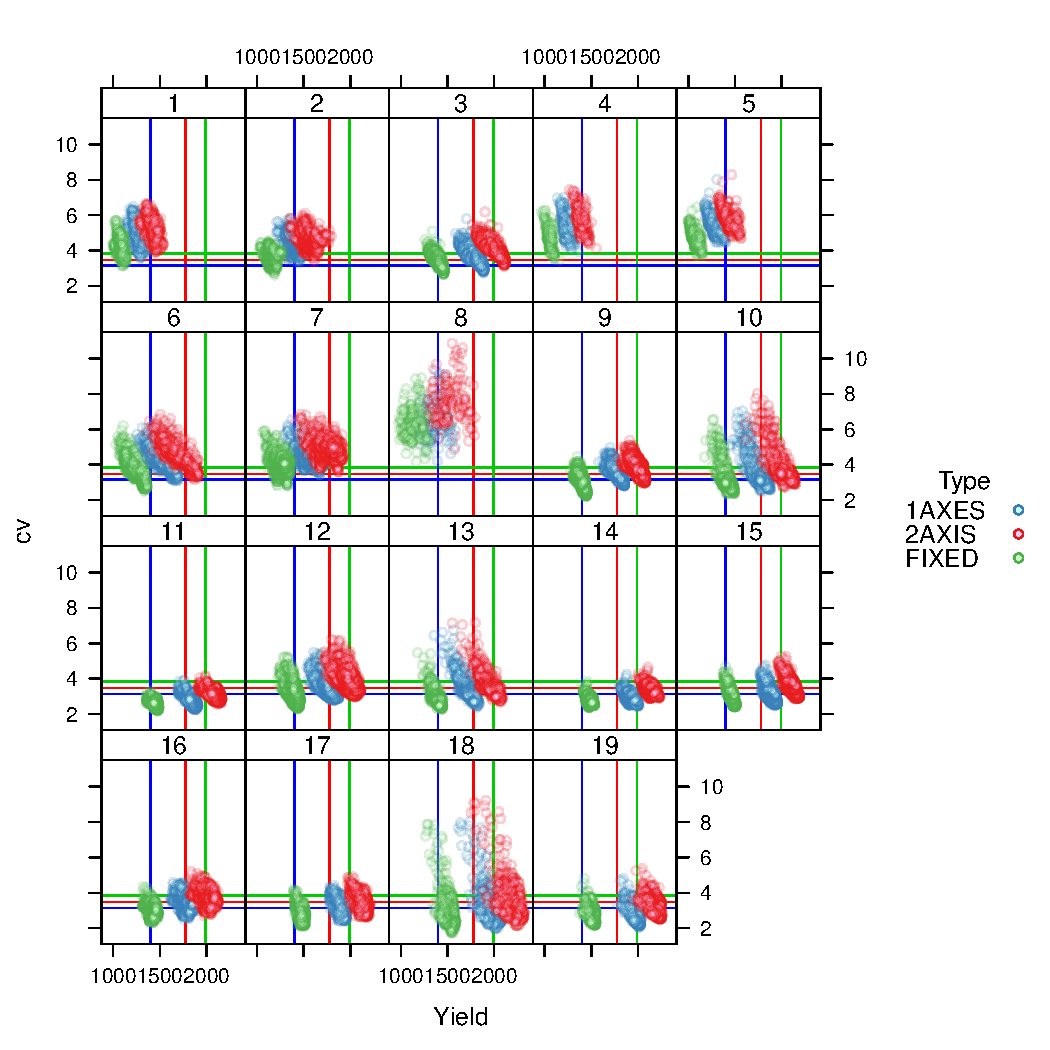
\includegraphics[width=\textwidth]{figs/capitulo5/Yearlycv_productivity3.pdf}
%   \caption{Yearly mean of PV yield $[\frac{kWh}{kWp}]$ (horizontal axis) and CV (vertical axis in percentage) by cluster and tracking system. The individual points correspond to individual grid points forming part of the clusters. Transparency of dots is applied to show importance of the number of points inside the clusters regarding its value of CV.}
%   \label{yearly_productivity_and_CV}
% \end{figure}

\subsection*{Complementarity}


Figure \ref{correlaciones_30} represents the correlation matrix, for each month and for all pairs of clusters, of the solar global irradiation at the horizontal plane, considering the whole period (1983-2013). Correlation coefficient varies in the annual cycle for each pair of clusters. Most of the relationships show a high positive correlation coefficient. This is the case particularly for northern clusters (4, 5, 6), which are highly correlated for every month. For clusters in the southern half of the Iberian Peninsula, from 14 to 19, the correlation coefficient is also positive, although it decreases in July and August for most of the pairs. 

However, the high positive correlation is not general. Northern clusters 4 and 5 are slightly correlated, not correlated or slightly positive correlated with southern clusters (14 to 19) for every month. This pattern is amplified in November, where the highest anti-correlation values are found between clusters 5 and 17 and between clusters 5 and 18. This negative correlation is statistically significant, in contrast to other cases with negative correlation. The absence of positive correlation between southern and northern clusters is more evident between clusters 17 and 18, at the south-east of the IP, and clusters 1 to 5 in the north. Overall, southern and eastern clusters are uncorrelated at least during part of the year with northern and northwestern clusters. In some cases, the absence of correlation is found between nearby clusters: in winter months, the north-eastern cluster 11 (central Ebro valley) is uncorrelated to the closely-lying clusters 4, 5 and 8 (in the northern coast and Pyrenees). This is probably related to persistent atmospheric situations with north to north-westerly winds, that cause cloudiness in the windward clusters and clear skies in the leeward Ebro cluster, due to a Föhn effect.


\begin{figure} [h!]
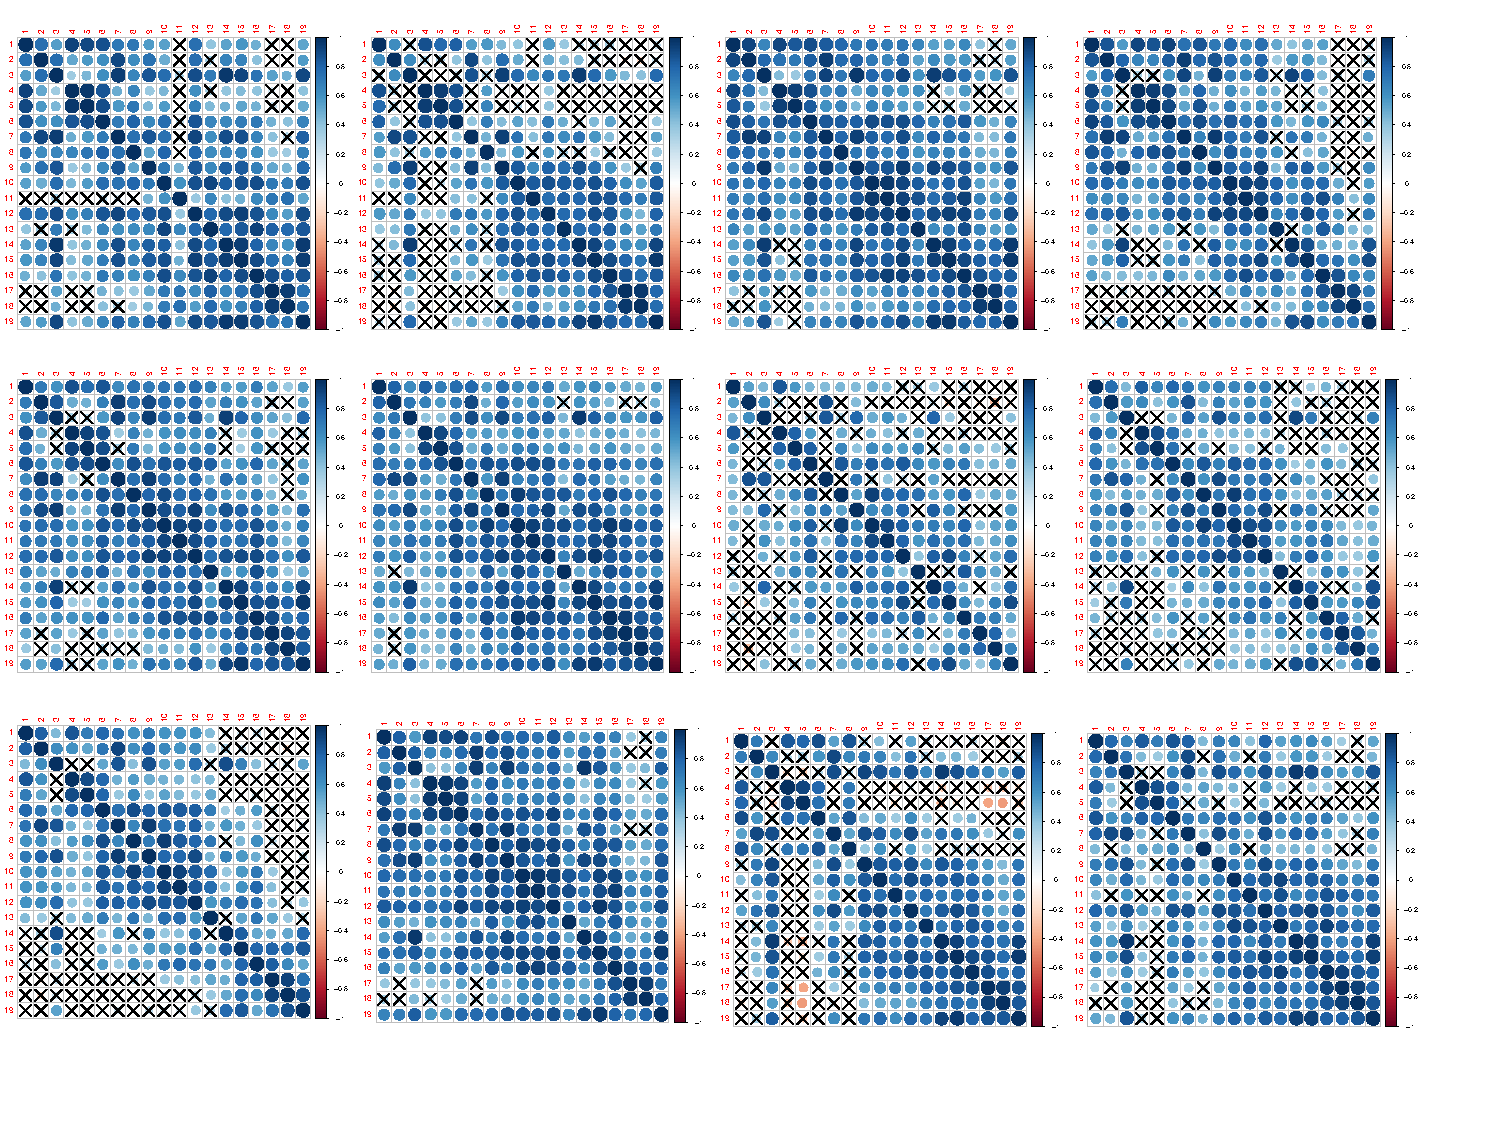
\includegraphics[scale=0.6]{figs/capitulo5/correlaciones_30.pdf}
\caption[Correlation matrix between clusters over the Iberain Peninsula]{Correlation matrix of the monthly time series for the period 1983-2013, between all pairs of clusters. First row: January to April, second row: May to August, third row: September to December. Circle’s size means significance of the correlation and the color bar represents the positive correlations in blue and negative correlations in red. Crosses indicate that correlation is not statistically significant. Row and column numbers are cluster numbers.}
\label{correlaciones_30}
\end{figure}

% \section{Monthly series variability}


% The annual cycle of CV is represented in \ref{cicloAnualCV_all} for solar irradiation and PV production. Although flatter cycles appear in some clusters, at the north-eastern part of the IP, a clear seasonality is observed in most cases, with a minimum for summer months. There are substantial differences between clusters, with the highest CV values in the northern ones.

% Regarding solar irradiation variability, it is also important to notice the differences in winter months between the eastern and north-western side of the Iberian Peninsula. Eastern clusters (10, 11, 13, 16, 17, and 18), have smaller values of CV (below $15\%$) in winter than northern and north-western clusters (1, 2, 3, 4 and 7), where values above $15\%$ and close to $20\%$ are found. In summer there is a different behavior because the main differences exist between the north and the south of the Iberian Peninsula. Northern clusters (1, 2, 4, 5 and 8) show summer CV values above $7\%$, while southern clusters (15, 14, 17, 18 and 19) show very low values, around $2\%$.

% Cluster 8, in the Pyrenees region has really high values in winter, above $25\%$. Its annual cycle has a wide range between winter and summer, decreasing to $7\%$ in August. On the other hand, north-eastern clusters (13, 11, and 10) show the smallest differences between winter and summer for the CV of solar irradiation.


% \begin{figure}
% 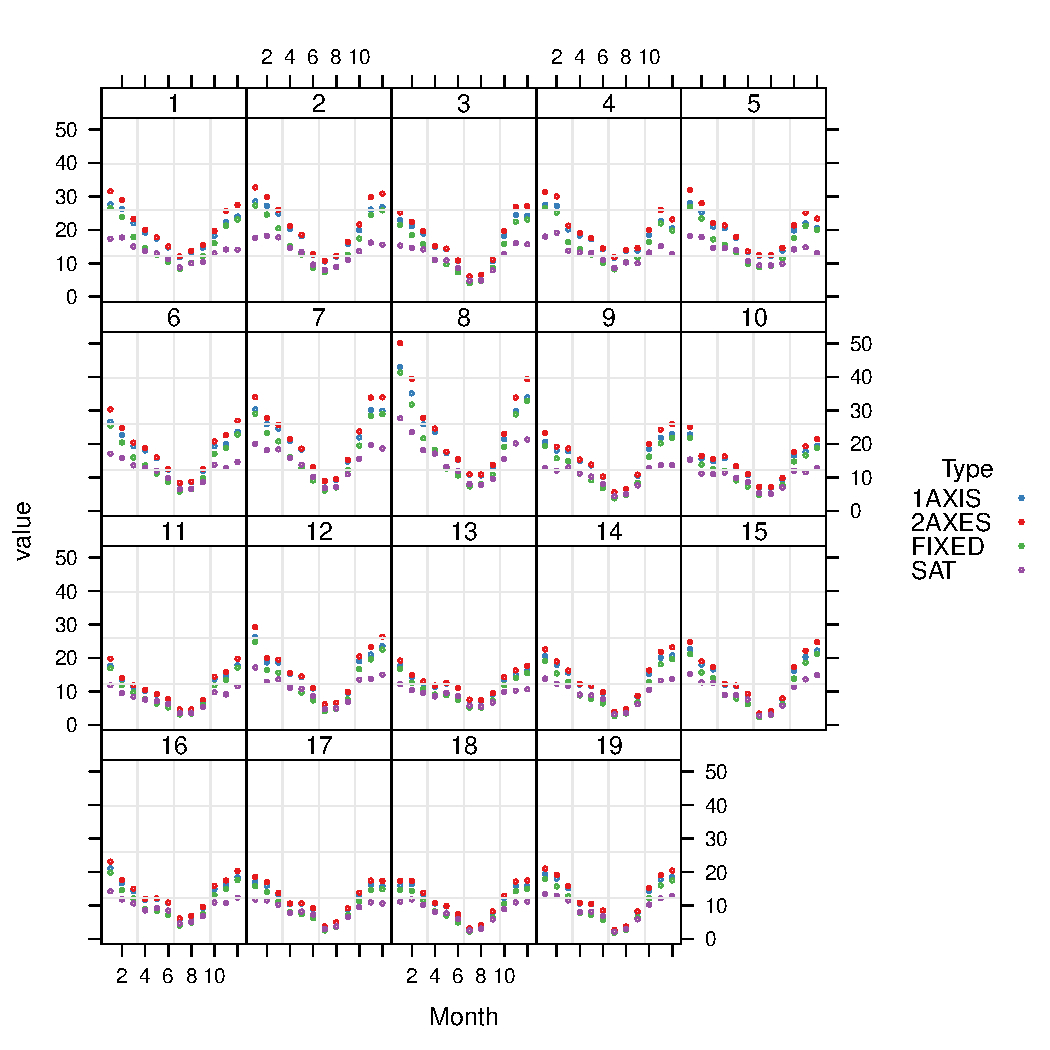
\includegraphics[width=0.9\textwidth]{figs/capitulo5/ciclo_anual_byCluster_all}
% \caption{Annual cycle of CV by cluster and for each tracking type and global solar irradiation at the horizontal plane.}
% \label{cicloAnualCV_all}
% \end{figure}


% \section{Complementarity}


% Figure \ref{correlaciones_30} represents the correlation matrix, for each month and for all pairs of clusters, of the solar global irradiation at the horizontal plane, considering the whole period (1983-2013). Correlation coefficient varies in the annual cycle for each pair of clusters. Most of the relationships show a high positive correlation coefficient. This is the case particularly for northern clusters (4, 5, 6), which are highly correlated for every month. For clusters in the southern half of the Iberian Peninsula, from 14 to 19, the correlation coefficient is also positive, although it decreases in July and August for most of the pairs. 

% However, the high positive correlation is not general. Northern clusters 4 and 5 are slightly correlated, not correlated or slightly positive correlated with southern clusters (14 to 19) for every month. This pattern is amplified in November, where the highest anti-correlation values are found between clusters 5 and 17 and between clusters 5 and 18. This negative correlation is statistically significant, in contrast to other cases with negative correlation. The absence of positive correlation between southern and north clusters is more evident between clusters 17 and 18, at the south-east of the IP, and clusters 1 to 5 in the north. Overall, southern and eastern clusters are uncorrelated at least during part of the year with northern and northwestern clusters. In some cases, the absence of correlation is found between nearby clusters: in winter months, the north-eastern cluster 11 (central Ebro valley) is uncorrelated to the closely-lying clusters 4, 5 and 8 (in the northern coast and Pyrenees). This is probably related to persistent atmospheric situations with north to north-westerly winds, that cause cloudiness in the windward clusters and clear skies in the leeward Ebro cluster, due to a foehn effect.


% \begin{figure} [h!]
% 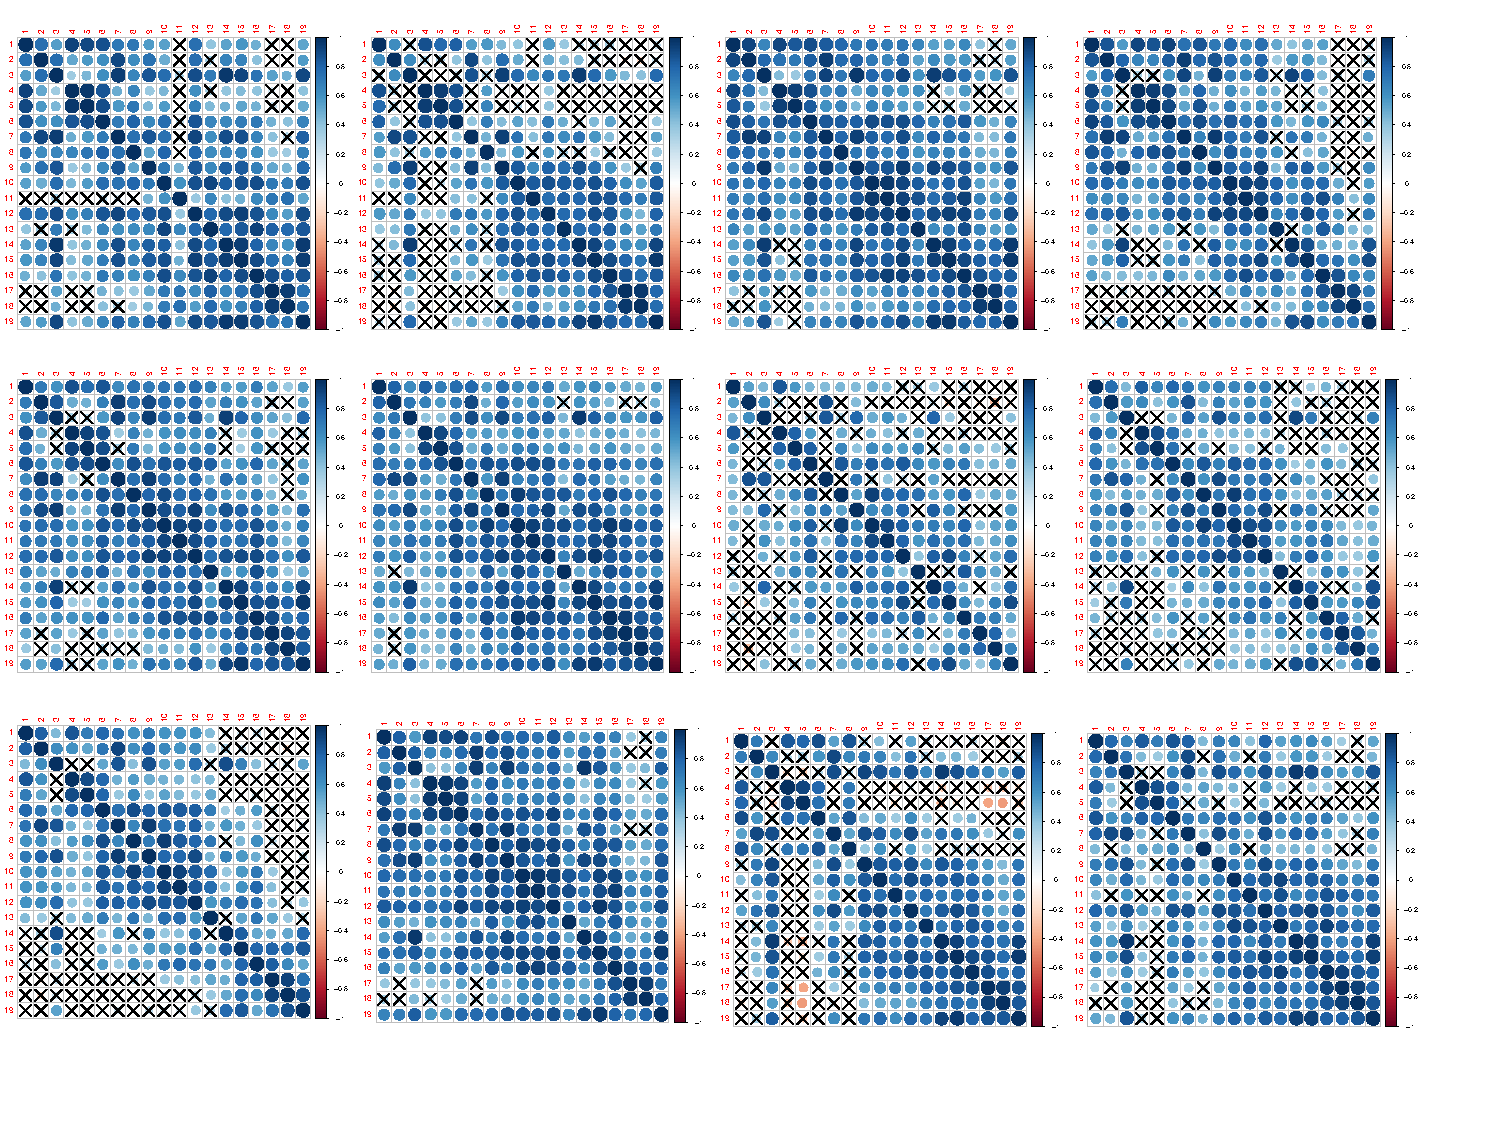
\includegraphics[scale=0.5]{figs/capitulo5/correlaciones_30}
% \caption{Correlation matrix of the monthly time series for the period 1983-2013, between all pairs of clusters. First row: January to April, second row: May to August, third row: September to December. Circle’s size means significance of the correlation and the color bar represents the positive correlations in blue and negative correlations in red. Crosses indicate that correlation is not statistically significant. Row and column numbers are cluster numbers.}
% \label{correlaciones_30}
% \end{figure}

%\end{subappendices}

\clearpage

%%%%%%%%%%%%%%%%%%%%%%%%%%%%%%%%%%%%%%%%%%%%%%%%%%%%%%%%%%%%%%%%%%%%%%%%%%%%%%%%%%%%%%%%%%

\chapter[Impact of aerosols on photovoltaic production]{Impact of aerosols on photovoltaic energy production over the Euro-Mediterranean area\label{cha:impact}}

\blfootnote
{This chapter shows the results of the paper published in Solar Energy journal: \textit{Impact of aerosols on the spatiotemporal variability of photovoltaic energy production in the Euro-Mediterranean area.}\\
https://doi.org/10.1016/j.solener.2018.09.085}


\begin{abstract}

%%  The increase in the photovoltaic energy installed capacity over the world leads to the need of a better understanding of solar resource and its variability.

  The aim of this work is to assess the influence of aerosols on photovoltaic energy production from seasonal to multi-decadal time scales. For this purpose we use various coupled aerosol-climate simulations that take into account the complex spatial and temporal patterns of natural and anthropogenic aerosols over the Euro-Mediterranean domain.

The results show that aerosols strongly influence the spatial pattern, seasonal cycle and long-term trend of PV production. The most affected area is Central Europe where sensitivity of PV production to aerosols is higher. The annual production loss due to aerosols ranges from no impact to $-16\%$ in The Netherlands, with variation depending on the area and on the typology of the tracking system. The summer production loss can even reach $-20\%$ over regions of Africa and Syria-Iraq.  

We conclude that aerosols cannot be neglected in the assessment of PV production at large time scales over the Euro-Mediterranean area. Besides, the potential increase in energy due to reduction in the antrophogenic aerosols is shown in the simulation of the brightening period over Europe, with an increase of 2000 ${\kilo\watthour\over\kilo\wattpeak}$ in a PV lifetime for the most affected areas. It illustrates the evolution that PV potential could follow in highly polluted areas through the effective implementation of pollution control measures.  
  
   
\end{abstract}
 
% \begin{keyword}
% \texttt{Photovoltaic production variability\sep Aerosols\sep Regional Climate Modeling}
% \end{keyword}

%\end{frontmatter}

%\linenumbers

\section{Introduction}


%In the last decades there has been an overall increase in the deployment of photovoltaic (PV) power plants over the world, demanding research in the fields that contribute to a better integration of this technology into the electricity system. Due to the variability of solar resource, a comprehensive study of its spatiotemporal behavior is needed.

Aerosols particles influence the climate system directly, affecting the Earth’s radiation budget by scattering or absorption of solar radiation, or indirectly, changing cloud properties. Due to their importance in the amount of solar radiation that reaches the Earth’s surface and their effect in the changing climate, the evaluation of their impact on the solar resource for energy purposes is of special interest.

A general lack of well-spread surface stations, previously commented, which provide solar radiation measurements, has made the satellite information the main and most reliable source of data up to now, due to its spatial and time resolution \cite*{Posselt2012, Ineichen2014}. However, satellite retrievals were not available several decades ago and they do not allow to quantify the effect of specific factors on solar irradiance. Thus for investigating long-term statistics and to disentangle the various factors influencing solar resource, a different approach is needed. Models are the best tool to understand processes that occur in the atmosphere and their link with the resource variability, as individual factors can be included or removed in them, allowing the isolation of their effects.

Due to the increasing concern about the availability of renewable energy resources under climate change scenarios, climate modeling has revealed itself as a valuable tool for evaluating future energy potential \cite*{Crook2011, Gaetani2014, Gaetani2015, Jerez2015, Jerez2015climix, Tobin2016}. However, representation of the clouds is still one of the main challenges for these models, and the spatio-temporal variability of aerosols is rarely taken into account in some of regional climate models \cite*{Bartok2017}, which could lead to significant errors in PV power forecasting or future energy estimations \cite*{Rieger2017}. Such climate simulations have to be combined with an accurate PV model capable of reproducing the system performance. Existing studies analyzing the influence of aerosols on solar irradiation lack spatial detail (because of the use of relatively coarse global climate models) and/or do not apply a detailed PV production model \cite*{Bergin2017}. 

The Mediterranean region is considered as highly influenced by aerosols coming from different sources \cite*{Lelieveld}. These aerosols have a deep impact on the climate of the region \cite*{Nabat2014, Nabat2015}, thus on the shortwave solar radiation reaching the surface \cite*{Mallet2016}. Regarding possible changes in antrophogenic aerosols in the future \cite*{Gaetani2014, Jimenez-Guerrero2011}, the relevance of the near-term climate change scenarios and the expected PV deployment, the study of the Euro-Mediterranean area is important for solar energy.

In this work we use a regional climate model \cite*{Nabat2014} with a realistic aerosol representation combined with an accurate PV model \cite*{Perpinan2012}. The influence of these aerosols in the spatiotemporal variability of PV production over the region is quantified. The analysis is made in present climate conditions for simulations between 2003 and 2009 and different tracking types are considered in the study, due to the different sensitivity of each typology to changes in solar radiation \cite*{Gutierrez2017}. On the other hand, the impact that trends in antrophogenic aerosols have in PV energy production is also investigated using longer simulations for the ``brightening'' \cite*{Wild2005} period, 1980-2012, reflecting how pollution control policies could benefit the PV energy production in highly polluted areas.

This chapter is organized as follows: in section 6.2 the climate and the photovoltaic model are described. In addition, there is a description of the aerosols and the datasets used for evaluation. Section 6.3 presents the results and shows the impact of aerosols on photovoltaic energy production. It is organized depending on the space-time scale analyzed and there is a subsection for the tracking system sensitivity.  Finally, section 6.4 is a discussion section for limitations and future perspectives and section 6.5 shows the main conclusions.

\section{Data and Methods}

Different climate simulations are used as an input of a PV power model. These climate simulations provide the daily-mean shortwave solar radiation, SSR, at the surface. The energy production model simulates the performance of a general photovoltaic system as in the previous chapter and includes different tracking types, considering the tilt of photovoltaic panels as a relevant component of the whole assessment. Computation of the photovoltaic energy model is made using the R open-source package named solaR \cite*{Perpinan2012}. Chapter \ref{cha:methods} explains in detail the methodology used for the photovoltaic model. 

\subsection{Climate Data}

The climate model used in this study (CNRM-RCSM4,\cite*{Sevault2014}) is a coupled Regional Climate System Model (RCSM) dedicated to the study of the Mediterranean climate. CNRM-RCSM4 is one of the RCSMs contributing to the multi-model Med-CORDEX initiative \cite*{Ruti2016}. It has the specificity to represent various components (atmosphere, land surface, river, ocean) of the Mediterranean regional climate system at high-resolution as well as their high-frequency coupling. The horizontal resolution is 50 km for the atmosphere, the land surface and the river network, and about 10 km for the Mediterranean Sea. In addition, the atmosphere part of the model, the so-called ALADIN-Climate version 5.2 \cite*{Colin2010} is one of the few available Regional Climate Models which can take into account a realistic representation of the spatiotemporal variability of the aerosols \cite*{Nabat2014}. The model has been extensively described, evaluated and inter-compared with other Med-CORDEX models in previous studies, \cite{Sevault2014, Nabat2013, Nabat2014,Flaounas2016, Gaertner2016, DellAquila2016, Harzallah2016, Cavicchia2016}

The detailed interannual aerosol dataset used in the climate simulations \cite*{Nabat2013}, NAB13, is able to reproduce the spatiotemporal variability of AOD (aerosol optical depth) over the Mediterranean region. It improves the representation of aerosols against older climatologies commonly applied in regional climate studies like Tegen \cite*{Tegen1997} or Tanré \cite*{Tanre1984}.

The NAB13 dataset includes five different aerosol species: Sea Salt, Black Carbon, Sulfate, Organic Carbon and Desert Dust (ss, bc, su, or, sd) with spatial and temporal variability. It is based on a blending of a satellite-derived AOD product and a high-resolution regional climate model using up-to-date interactive aerosols module. This dataset has also been evaluated against ground stations \cite*{Nabat2013}.

During the eighties, some policies against the emissions of certain types of anthropogenic aerosols were implemented in Europe, which has been linked with the observed increase in the shortwave solar radiation in the area \cite*{Wild2005}. For simulations over this commonly named ``brightening period'' (1980-2012), a trend for sulfate aerosols is included in NAB13, being able to reproduce the shortwave solar radiation trend observed over Europe since 1980 \cite*{Nabat2013}.

There is a large spatial and seasonal variability of the AOD at 550nm over the Euro-Mediterranean. Spring and summer months are highly influenced by dust aerosols in the south of the domain. In winter, anthropogenic aerosols dominate in central Europe and during autumn, there are few areas with high values in opposition to the rest of the domain.

The domain considered in the simulations covers the Mediterranean area in addition to a large part of Europe (see Figure \ref{fig:mapapral}).

For the first period, 2003-2009, a pair of runs is analyzed. We refer to them as \textbf{AER} and \textbf{NO-AER}. The AER simulation includes the NAB13 dataset, whereas no aerosols are included in NO-AER. This pair allows to easily attribute the obtain differences to the aerosols effect, therefore to quantify the impact of aerosols on the Euro-Mediterranean SSR and PV productivity. It is an important point considering the fact that some of the state-of-art RCMs do not include aerosols in their simulations, so it gives an idea of that missing forcing.

Secondly, a longer simulation between 1980 and 2012, \textbf{TREND}, covering the ``brightening'' period observed in Europe is also analyzed. It will show the effect of a decreasing trend in sulfur aerosols on the shortwave solar radiation and on the PV productivity.  

A summary of the different simulations is reported in Table \ref{tabSIM}.

\begin{table}
  \begin{tabular}{>{\raggedright}m{2cm}>{\raggedright}m{3cm}>{\raggedright}m{2cm}}
    \toprule 
    Simulation & Aerosols & \centering{Period}\tabularnewline
    \midrule
    AER & NAB13 & 2003-2009
    \tabularnewline
    \midrule
    NO-AER & Not included & 2003-2009
   \tabularnewline
   \midrule           
  TREND & NAB13 + sulfates trend & 1980-2012
   \tabularnewline
    \bottomrule
  \end{tabular}
  \caption[Simulations of the CNRM-RCSM4 used as input of the PV model, period and aerosols representation]{Simulations of the CNRM-RCSM4 regional climate model to obtain SSR and temperature as input of the photovoltaic model, period and representation of aerosols in each simulation.}
\label{tabSIM}
\end{table}

\begin{figure}[h!]
\centering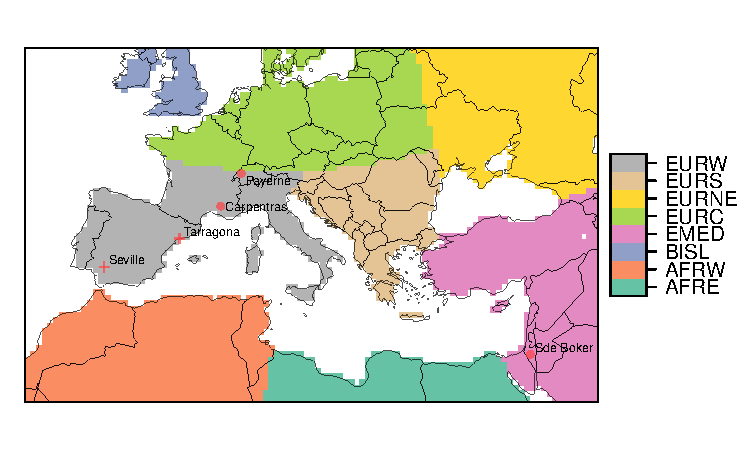
\includegraphics[width=0.7\textwidth]{figs/capitulo6/zonasPuntosLabel.pdf}
\caption[Euro-Mediterranean areas defined and local points]{Areas defined to evaluate the difference in solar radiation between the satellite and the climate model simulations: Western Europe, EURW; Southern Europe, EURS; North-Eastern Europe, EURNE; Central Europe, EURC; Eastern Mediterranean, EMED; British Island, BISL; Western Africa, AFRW; Eastern Africa, AFRE. The location of the BSRN stations is represented with points ``.'' and the two PV plants are plotted with ``+'' in orange.}
\label{fig:mapapral}
\end{figure}

 
\subsection{PV model description}

As in the previous chapter, the PV model described in \ref{cha:methods} is used with the SSR from the climate model as the input. The procedure is described in \cite{Perpinan2009} and the same methodology was applied in \cite{Gutierrez2017}. In this section we make use of the commonly used terms in the PV model description: the shortwave solar radiation, SSR, from the climate model is equivalent to the global irradiation at the horizontal plane $G(0)$, which is composed of the beam component, $B(0)$, the diffuse irradiation, $D(0)$, and the albedo $R(0)$.

% A photovoltaic energy system is mainly composed of the generator, consisting of several modules that include the cells to transform solar radiation into electricity, and the inverter, which transforms direct current into alternate current to be integrated into the electricity network. The assessment or estimation of the power output of a PV system implies modeling its components. For this purpose, two main steps have to be considered. The first is related to the amount of energy that reaches the generator surface and the other is based on the performance of the electrical components. The procedure is described in \cite{Perpinan2009} and the same methodology was applied in \cite{Gutierrez2017} .

The two steps followed to obtain the PV output are:

1) Global irradiation at the horizontal plane $G(0)$, as an output of the climate model, has to be transformed into the global effective irradiation, $G_{eff}(\alpha, \beta)$, which is the amount of energy reaching the tilted surface of the generator (where $\alpha$ is the azimuth angle and $\beta$ the inclination angle) after considering reflection losses, angle of incidence and accumulated dust.  

% First, for the decomposition of $G(0)$, empirical equations that correlates the \textit{clearness index} and the \textit{diffuse fraction} \cite*{Page1961} are used. The clearness index is a measure for the energy lost when solar irradiation goes through the atmosphere, and the diffuse fraction is the relationship between the diffuse component, $D(0)$, and the global irradiation at the horizontal plane $G(0)$. Its value is the amount of the diffuse component in global irradiation.

% The equations that relate the clearness index to the diffuse fraction depend on the place and time scale involved. There are many relationships proposed depending on the area of the study \cite*{deMiguel2001, Gopinathan1995}. For daily time-scales, the equations that relate the clearness index and the diffuse fraction proposed by \cite{Aguiar1992} are used in our case. 

Three different tracking types are considered also here for the photovoltaic generator. The equations describing movements and relative position between the system and the sun are described in \cite{Perpinan2009}

\begin{enumerate}
\item \textbf{Fixed panels} with an optimum angle of inclination that depends on the latitude.
\item \textbf{One} axis trackers, with a generator rotating on an axis oriented North-South. We will refer to them as \textbf{“one”}.
\item \textbf{Two-axes} tracking system that allows variation of the azimuth and inclination angles, we will refer to them as \textbf{“two”}.
\end{enumerate}

To obtain irradiation components in the tilted surface at daily time scale, it is first necessary to estimate the irradiance profile using empirical relationships \cite*{Collares-Pereira1979}. The irradiance profile is then transformed into its components at the tilted surface and integrated in time to obtain the energy reaching the generator surface. Direct irradiance can be transformed to the tilted surface using only geometrical criteria whereas the diffuse fraction is obtained with the model proposed by \cite{hay1985estimating}. This model considers an approximation where the sky sphere is seen by the generator as isotropic except for the circumsolar region, which is considered to emit direct irradiance. The albedo component is considered as isotropic, due to the fact that its contribution to global irradiance is low. 

Finally, we apply equations from \cite{Martin2001} to obtain $G_{eff}(\alpha, \beta)$. It includes optical losses due to the fact that, except for the two-axis tracking system, the incident irradiation deviates from the normal of the generator. Also, transmittance losses are included for accumulated dust over the surface, considering a ``moderate dust degree'' in the terms used in the referenced paper \cite{Martin2001}. In this case, any spatial distinction is considered and the same coefficient values are used to calculate angular and transmittance losses. 

2) The second step is the transformation into power output, depending on the electrical characteristics of the components in the photovoltaic system and second order effects like temperature. Detailed information about this step can be found in the Methods chapter and in \cite{Perpinan2009}.

%Ambient temperature is needed since the efficiency of the cells decreases with the increase of temperature, assuming a linear relationship. In this work we use the equation of \cite{Crook2011}, to calculate the daytime temperature from the daily maximum and minimum temperature, obtaining a daily profile. 

% %Computation of the photovoltaic energy model is carried out with the \texttt{solaR} package \cite*{Lamigueiro2012}. This package implements in R a set of functions that include the sun apparent movement equations, the solar irradiation and irradiance decomposition, transposition models, and the PV generator and inverter models. 

% % \begin{table}[h!]
% %   \begin{tabular}{>{\raggedright}m{2cm}>{\raggedright}m{6cm}}
% %     \toprule 
% %     Element & Method\tabularnewline
% %     \midrule
% %     PV generator & Identical modules with
% %     $dV_{oc}/dT_{c}=0,475\frac{\%}{\celsius}$ and $NOCT=47\celsius$. 
% %     The MPP point calculated as in \cite{garcia2005caracterizacion}). \tabularnewline
% %     \midrule
% %     Inverter & Efficiency equation proposed in
% %     \cite{jantsch1992results}:  
% %     \begin{equation}
% %       \eta_{inv}=\frac{p_{o}}{p_{o}+k_{0}^{o}+k_{1}^{o}p_{o}+k_{2}^{o}p_{o}^{2}}
% %     \end{equation}
% %     where $p_{o}=P_{ac}/P_{inv}$ is the normalized output power of the inverter. The characteristic coefficients of the
% %     inverters are: $k_{0}^{o}=0.01$, $k_{1}^{o}=0.025$, $k_{2}^{o}=0.05$.\tabularnewline
% %     \midrule
% %     Other losses & \begin{itemize}
% %     \item Average tolerance of the set of modules, $3\%$.
% %     \item Module parameter dispersion losses, $2\%$.
% %     \item Joule losses due to the wiring, $1.5\%$.
% %     \item Average error of the MPP algorithm of the inverter, $1\%$.
% %     \item Losses due to the MV transformer, $1\%$.
% %     \item Losses due to stops of the system, $0.5\%$.
% %     \end{itemize}
% %     \tabularnewline
% %     \bottomrule
% %   \end{tabular}
% %   \caption{Calculation procedure for the estimation of energy produced by a PV system from daily global horizontal irradiation data. Left column represents the element of the PV system and the right column the equations and methods used in each case for the efficiency of the elements.}
% %   \label{table1}
% % \end{table}

\subsection{Datasets for evaluation}
\subsubsection{Satellite product: CM-SAF.}

% CM-SAF (Climate Monitoring Satellite Application Facility) \cite*{Schulz2009} was created as part of EUMETSAT Satellite Application Facility (SAF) when the importance of “contributing to the operational monitoring of the climate and the detection of global climatic changes” was recognized. Besides its operational products, they provide Climate Data Records generating long-term data, which is a valuable product for climate variability studies.

The SARAH \cite*{Muller2015} dataset for daily shortwave solar radiation, SSR, is used with a horizontal resolution of 0.44º to be consistent with the model simulations and for the period 2003 and 2009. For this product, the $85\%$ of absolute differences with shortwave solar radiation measurements is below 10 $\watt/m^2$ for monthly values and 13 $\watt/m^2$ for daily means.

Concerning aerosols representation, the satellite dataset includes information from MACC \cite*{Benedetti2009, Morcrette2009}, provided by the European Centre for Medium-Range Weather Forecasts (ECMWF). Monthly long-term means of a 0.5x0.5 degrees grid are spatially interpolated to assign the values of each pixel.

\subsubsection{BSRN stations}

%The BSRN (Baseline surface radiation network) \cite*{Ohmura1998} is a set of ground-based measurements, from the WRCP Radiative Fluxes Working Group. It was created for supporting research in the radiation budget of the Earth-atmosphere and the radiation distribution, considering its main role in climate processes. The main objective is to provide high-quality measurements that are able to deal with the scarcity of the existing radiometric network. Although there are not many stations available for the period of the study in the Euro-Mediterranean domain, the high quality data provided by BSRN is necessary for a first evaluation of the climate simulations.

The three stations of the BSRN network used in this study (Payerne, Carpentras and Sede Boker) covered the period 2003-2009 and provide SSR monthly data \cite*{Konig-Langlo2013}. Their location is represented in Figure \ref{fig:mapapral} together with the PV plants considered in the study.   

\subsubsection{Temperature data: ECAD}

The PV production assessment calculated using the SSR from satellite data needs also the temperature for the performance of cells inside the module. The gridded E-OBS data set from the EU-FP6 project ENSEMBLES \cite*{Haylock2008} is used in the energy production model at daily resolution. Mean, maximum and minimum temperature from the dataset, in a spatial resolution of 0.25º, are interpolated to the same grid of the climate model. 

\subsubsection{PV production data}

Data from two different power plants are used for the evaluation of the simulated PV power and the assessment of the added value of the aerosol inclusion in the climate simulations.

The two power plants are in the Iberian Peninsula and their location represented in Figure \ref{fig:mapapral}. The first one, located in Tarragona in the North-East area, is a PV system with fixed structure. The second one is a two-axis tracking PV plant located in Seville, in the South of Spain. Details of both PV power plants are in Table \ref{tabPlants}, including the electrical characteristics of their components. 

\begin{table}[h!]
  \begin{tabular}{>{\raggedright}m{1.5cm}>{\raggedright}m{3cm}>{\raggedright}m{3cm}}
    \toprule 
     & \centering{Seville} & \centering{Tarragona}\tabularnewline
    \midrule
    Type & \centering{two-axes} & \centering{fixed} 
\tabularnewline
    \midrule
    Generator & \centering{$P_{g}=27.31$ $\kilo\wattpeak$}\\ 
                 \centering{$N_{mp}=12$}\\
                 \centering{$N_{ms}=11$} & \centering{$P_g=100.18$ $\kilo\wattpeak$}\\
                               \centering{$N_{mp}=27$}\\
                               \centering{$N_{ms}=35$}
   \tabularnewline
   \midrule
   Inverter & \centering{$P_{inv}=25$ $\kilo\watt$}\\
              \centering{$V_{min}=405$ $\volt$} & \centering{$P_{inv}=100$ $\kilo\wattpeak$}\\
                                \centering{$V_{min}=450$ $\volt$}
    \tabularnewline    
    \bottomrule
  \end{tabular}
  \caption[Electrical components of the PV power plants]{Summary of the electrical components of the two photovoltaic plants, including generator characteristics (generator power $P_g$, and modules in parallel and serie, Nmp and Nms) and the inverter characteristics (power of the inverter $P_{inv}$ and the voltage $V_{min}$).}
  \label{tabPlants}
\end{table}


Data of PV production are difficult to obtain due to confidentiality contracts. Moreover, when data are available time series are not always complete. Maintenance, modules substitutions, inverter problems and other stops in the production may lead to common time-gaps in the datasets. These limitations must be taken into account when establishing statistical comparisons between models and real data. In this case, the two PV power plants provide daily data within the period 2003-2009, the details are in Table \ref{localData}. Monthly means of these data are compared against the monthly means of simulated daily PV productivity, energy produced by the power installed ${\kilo\watthour\over\kilo\wattpeak}$, with the models and the satellite. Only months with more than 15 days of data available are considered for the monthly mean and compared against simulated data.

\section{Results} 

Although the AOD dataset and the climate simulations used in this study have already been evaluated against observations and satellite datasets in \cite*{Nabat2013, Nabat2014, Nabat2015}, an additional assessment of the SSR from the climate simulations is also made in this work against the CM-SAF SARAH dataset \cite*{Muller2015} for the period 2003-2009 and against some BSRN \cite*{Konig-Langlo2013} stations at a local scale. 

\subsection{Local scale}

Three different stations from BSRN cover the period between 2003-2009 with SSR monthly data. Stations are represented in Figure \ref{fig:mapapral} with points. Also, two different power plants in Spain, represented in Figure \ref{fig:mapapral} with a cross, are used to evaluate PV power simulations at a local scale. A summary of the data used in this section, the periods and the resolution can be found in Table \ref{localData}.


\begin{table}[h!]
  \begin{tabular}{>{\raggedright}m{2cm}>{\raggedright}m{2cm}>{\raggedright}m{2cm}>{\raggedright}m{2cm}>{\raggedright}m{2cm}>{\raggedright}m{2cm}}
    \toprule 
    Data from & \centering{Seville} & \centering{Tarragona} & \centering{Payerne} &\centering{Sede Boker} &\centering{Carpentras}\tabularnewline
    \midrule
    Variable & \centering{PV productivity} & \centering{PV productivity} & \centering{SSR} & \centering{SSR} & \centering{SSR} 
\tabularnewline
    \midrule
    Time res. & \centering{day} & \centering{day} & \centering{month} & \centering{month} & \centering{month}
                    \tabularnewline
   \midrule
                                                                                            Period & \centering{518 {\small{daily values between:}} 02-07-2007\\30-11-2008} & \centering{300 {\small{daily values between:}} 01-01-2003\\19-03-2005} & \centering{2003-2009} & \centering{2003-2009} & \centering{2003-2009}
                  \tabularnewline    
 \midrule
    $\%$ no data & \centering{0} & \centering{8 $\%$} & \centering{0} & \centering{10.71 $\%$} & \centering{0}
                    \tabularnewline

 \bottomrule
  \end{tabular}
  \caption[Summary of the local PV data from power plants and SSR from BSRN stations]{Summary of the local data of PV power plants and SSR from BSRN stations used for the evaluation of the simulations. SSR is evaluated as input of the PV model and the PV output as the result of the whole modeling process.}
  \label{localData}
\end{table}

In Figure \ref{fig:station} differences in monthly time series of SSR from simulations and satellite data and the stations measurements are represented.

\begin{figure}[h!]
  \centering\begin{subfigure}{0.45\textwidth}
    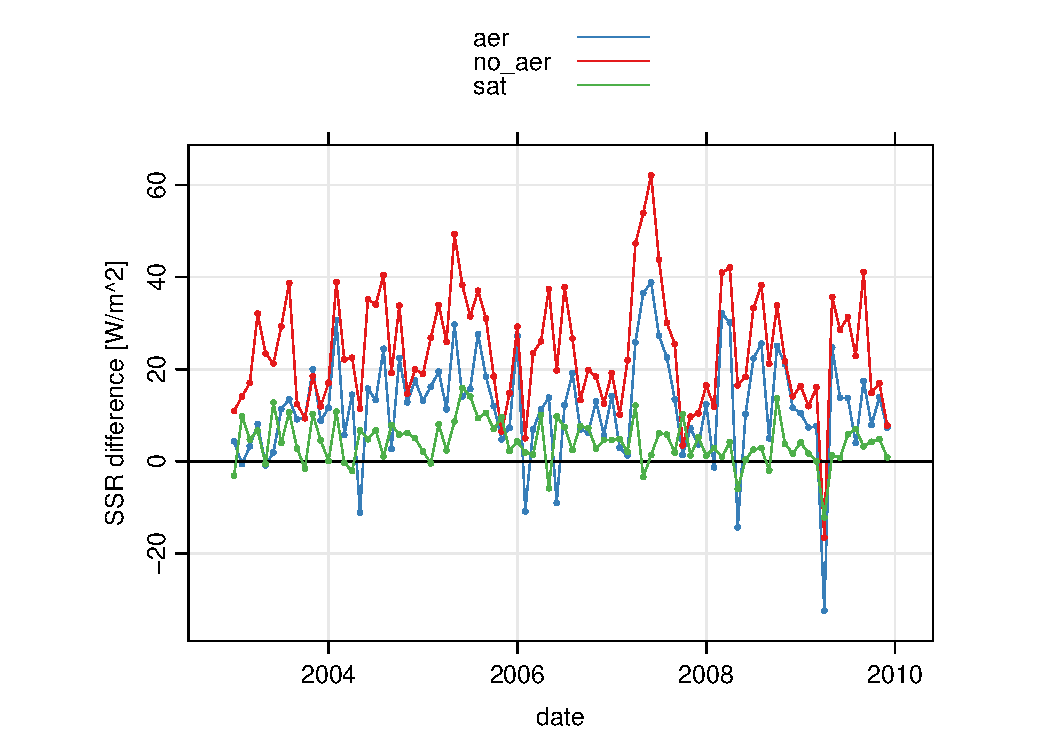
\includegraphics[width=1.25\textwidth]{figs/capitulo6/CarpentrasMesesDif.pdf}
    \caption{Carpentras}
    \label{Carpentras}
  \end{subfigure}
  %
  \centering\begin{subfigure}{0.45\textwidth}
    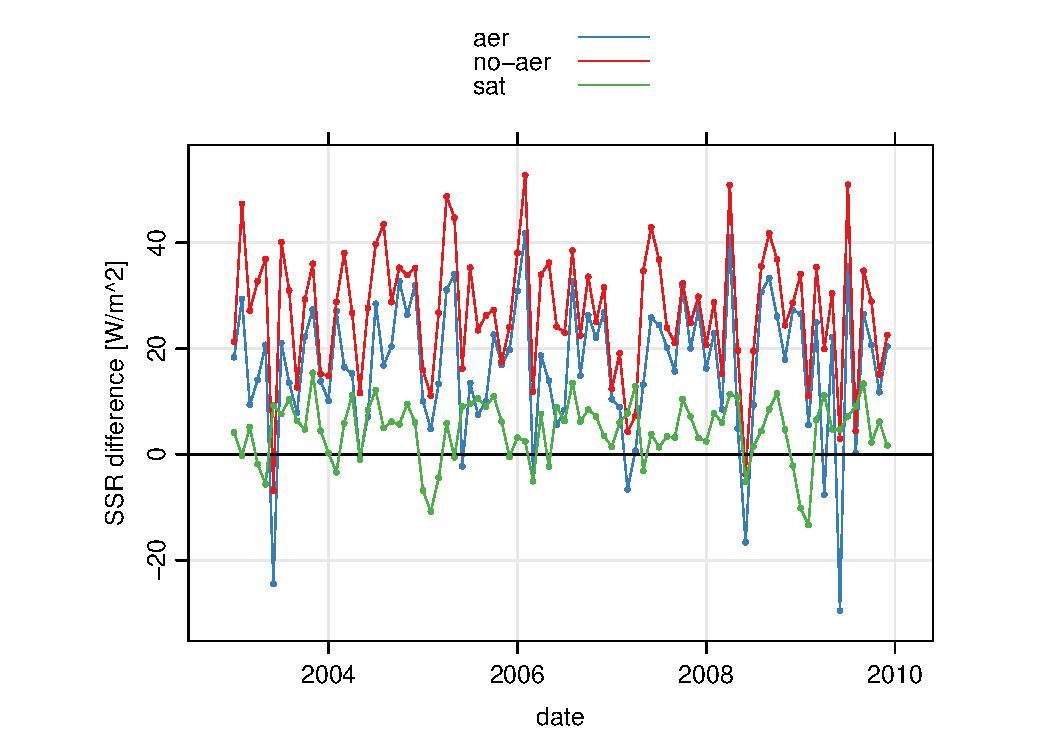
\includegraphics[width=1.25\textwidth]{figs/capitulo6/PayerneMesesDif.pdf}
    \caption{Payerne}
    \label{Payerne}
  \end{subfigure}
  %
    \centering\begin{subfigure}{0.45\textwidth}
    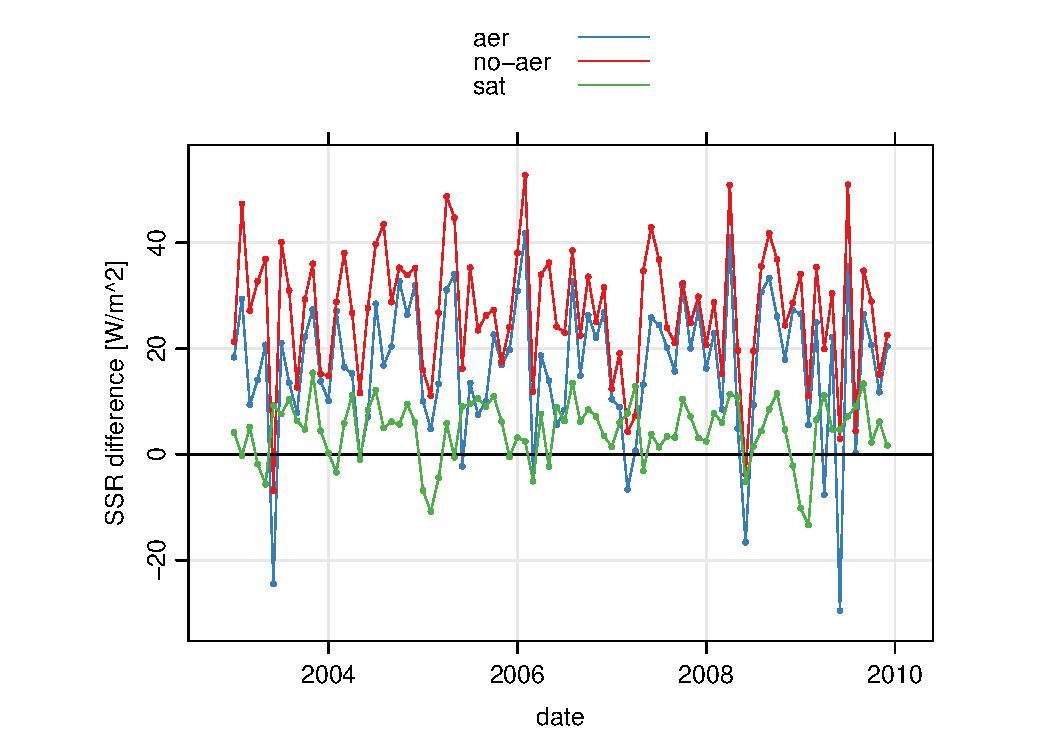
\includegraphics[width=1.25\textwidth]{figs/capitulo6/SedebokerMesesDif.pdf}
    \caption{Sede Boker}
    \label{fig:Sde Boker}
  \end{subfigure}
  \caption[Time series of differences between SSR from simulations, satellite data and BSRN stations]{Difference in SSR $\left[\si{\watt\per\metro\squared}\right]$ between both simulations and the satellite with respect to the data from BSRN stations (BSRN)}
    \label{fig:station}
\end{figure}

For the three stations, the satellite has better results than the simulations, although the error magnitude varies depending on the station. There is also a general improvement of the AER simulation against the NO-AER. Carpentras station is the one with lower bias with respect to the observed data \ref{Carpentras}. In the case of the Sede Boker station \ref{fig:Sde Boker}, there is a seasonal bias in the AER simulation. High negative differences appear from May to August, showing underestimation of the SSR in these months.

Several statistical measurements summarize the general performance of the SSR from the climate model and the PV simulations at each location and are reported in Table \ref{RMSE_MAE_table}.

For the simulation of PV power output, the daily mean of PV production data averaged for each month is compared with simulated PV energy production at each power plant, using the three possibilities of SSR data as input: AER, NO-AER and SAT. For these simulations, in order to help with the visualization of the results a \textit{violin plot} (\ref{violin}) is used to visualize the absolute error and its distribution.
For the Seville PV power plant \ref{fig:figuraSEVILLA}, AER performs better than NO-AER and SAT simulations showing lower errors. Besides, only AER has some negative errors, which means underestimation for some months, whereas the satellite and the NO-AER have only positive error values.

The median error for the AER simulation is less than 0.25 $\si{\kilo\watthour\per\kilo\wattpeak}$. Differences are concentrated around this value, which makes the distribution to peak around it in a narrow shape, although the range is wider due to higher values above 0.5 $\si{\kilo\watthour\per\kilo\wattpeak}$ that spread the distribution.

NO-AER simulation has a wider range of errors than AER and SAT, and a wider distribution. The satellite presents a median error close to 0.5 $\si{\kilo\watthour\per\kilo\wattpeak}$, as could be expected from the evaluation and report of the CM-SAF dataset.

\begin{figure}[h!]
  \centering\begin{subfigure}{0.45\textwidth}
    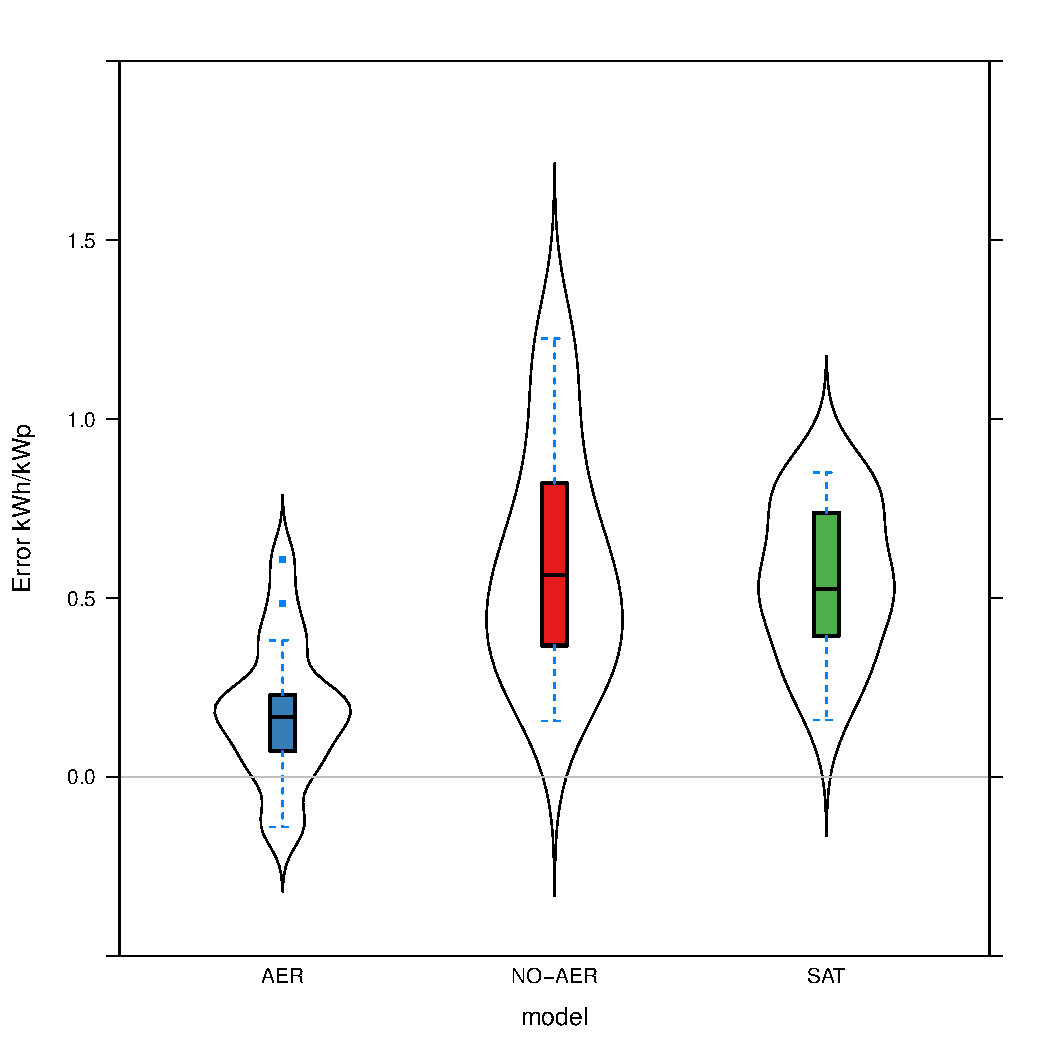
\includegraphics[width=1\textwidth]{figs/capitulo6/violinplorSeville.pdf}
    \caption{Seville}
    \label{fig:figuraSEVILLA}
  \end{subfigure}
  %
  \centering\begin{subfigure}{0.45\textwidth}
    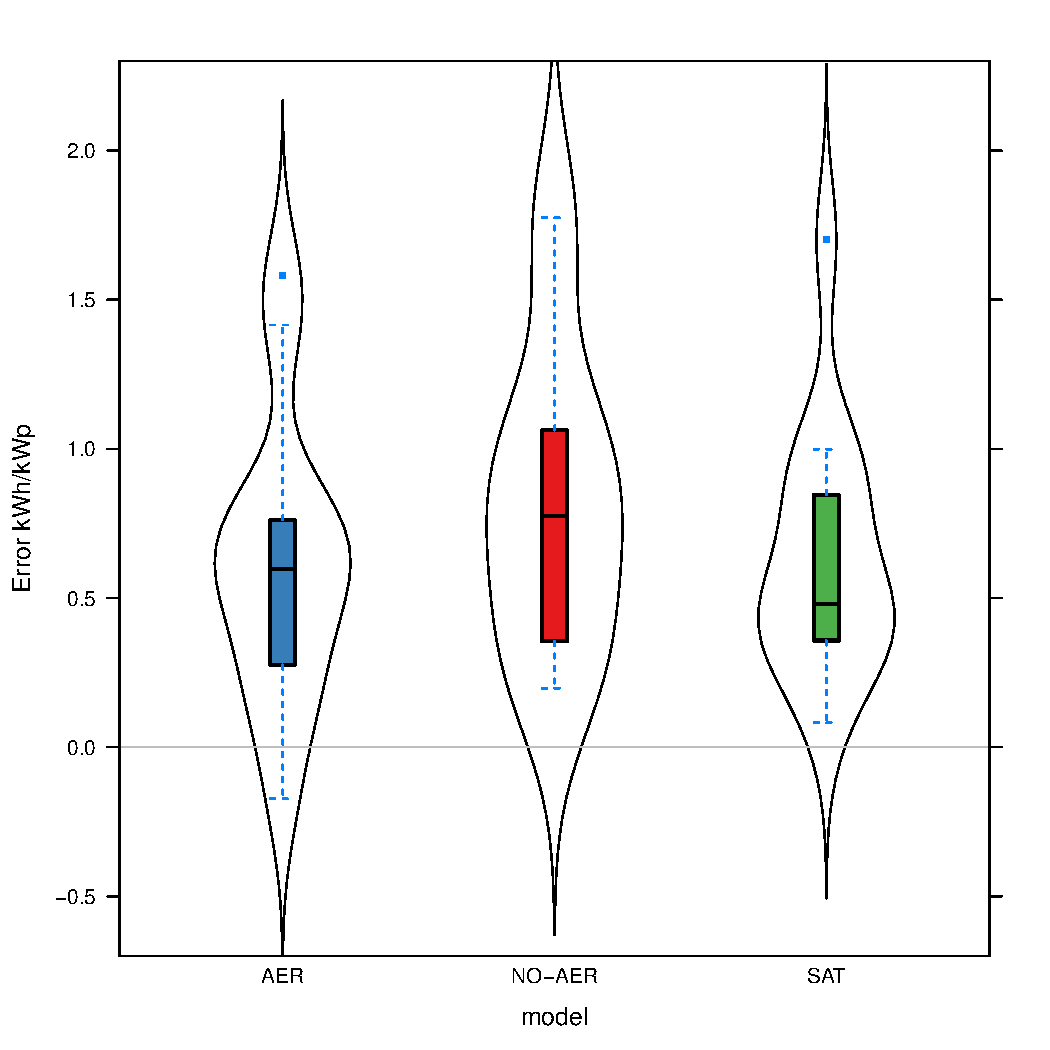
\includegraphics[width=1\textwidth]{figs/capitulo6/violinplotTarragona.pdf}
    \caption{Tarragona}
    \label{fig:violinTarragona}
  \end{subfigure}
  \caption[Distribution of differences in monthly mean of daily PV productivity between simulations and real PV data]{Distribution of differences in monthly mean of daily PV productivity $\left[\si{\kilo\watthour\per\kilo\wattpeak}\right]$ from Seville and Tarragona power plants and the simulated with the model, AER (blue) and NO-AER (red), and the satellite (green) in the same location. The period for Seville is from July 2007 to November 2008 and for Tarragona power plant from January 2003 to December 2005. The violin plot represents at the y-axis the probability density function of the variable, estimated with a kernel density estimation. Along this axis, the plot represents the shape of the variable distribution and it is duplicated by symmetry over an imaginary vertical axis to facilitate visualization. In this way it is easier to see not only statistical parameters represented in the boxplot, that it is also shown inside the violin, but also how the errors are distributed.}
    \label{violin}
  \end{figure}

\begin{table}[h!]
  \begin{tabular}{>{\raggedright}m{1.5cm}>{\raggedright}m{1.5cm}>{\raggedright}m{2cm}>{\raggedright}m{2cm}>{\raggedright}m{2cm}>{\raggedright}m{2cm}}
    \toprule 
    Location & \centering{Simulation} & \centering{RMSE} & \centering{MBE} &\centering{cor} &\centering{sd}\tabularnewline
    \midrule
    Seville & \centering{AER} & \centering{0.27} & \centering{0.18} & \centering{0.98} & \centering{1.34}
    \tabularnewline
    & \centering{NO-AER} & \centering{0.67} & \centering{0.60} & \centering{0.95} & \centering{1.29}
    \tabularnewline
    & \centering{SAT} & \centering{0.59} & \centering{0.55} & \centering{0.98} & \centering{1.45}
    \tabularnewline
   \midrule
    Tarragona & \centering{AER} & \centering{0.77} & \centering{0.61} & \centering{0.87} & \centering{1.21}
    \tabularnewline
    & \centering{NO-AER} & \centering{0.96} & \centering{0.82} & \centering{0.9} & \centering{1.29}
    \tabularnewline
    & \centering{SAT} & \centering{0.76} & \centering{0.64} & \centering{0.88} & \centering{1.13}
   \tabularnewline
   \midrule
  Payerne & \centering{AER} & \centering{21.21} & \centering{16.62} & \centering{0.97} & \centering{77.4}
  \tabularnewline
    & \centering{NO-AER} & \centering{29.70} & \centering{27.07} & \centering{0.98} & \centering{81.88}
  \tabularnewline                           
    & \centering{SAT} & \centering{7.36} & \centering{4.6} & \centering{0.99} & \centering{83.29}                         \tabularnewline
      \midrule
      Carpentras & \centering{AER} & \centering{16.59} & \centering{12.05} & \centering{0.98} & \centering{90.05}
  \tabularnewline
  & \centering{NO-AER} & \centering{27.26} & \centering{24.10} & \centering{0.99} & \centering{90.57}
  \tabularnewline
    & \centering{SAT} & \centering{6.38} & \centering{4.26} & \centering{1.00} & \centering{88.71}
 \tabularnewline
      \midrule
  Sede Boker & \centering{AER} & \centering{18.89} & \centering{8.17} & \centering{0.98} & \centering{62.83}
  \tabularnewline
  & \centering{NO-AER} & \centering{37.42} & \centering{35.63} & \centering{0.98} & \centering{76.06}
  \tabularnewline
    & \centering{SAT} & \centering{12.00} & \centering{10.27} & \centering{0.99} & \centering{77.62}
 \tabularnewline
 \bottomrule
  \end{tabular}
  \caption[Statistical analysis at local scale of the simulations with climate models]{Values for the root mean squared error (RMSE), mean bias error (MBE), temporal correlation (cor) and standard deviation (sd) for the simulated PV production in Seville power plant and Tarragona power plant compared with the final productivity data measured $\left[\si{\kilo\watthour\per\kilo\wattpeak}\right]$ and the SSR from the climate model simulations and the satellite in comparison with the SSR from BSRN stations $\left[\si{\watt\per\metro\squared}\right]$}
  \label{RMSE_MAE_table}
\end{table}

The Tarragona PV power plant presents larger errors. The SAT has slightly better performance than AER and the improvement with respect to NO-AER can be observed in both cases. 

AER simulation's median error is 0.60 $\si{\kilo\watthour\per\kilo\wattpeak}$ and NO-AER simulation error has larger values, the median is 0.77  $\si{\kilo\watthour\per\kilo\wattpeak}$. The SAT error has lower median value: 0.48  $\si{\kilo\watthour\per\kilo\wattpeak}$.

It can be also appreciated in Figure \ref{fig:violinTarragona} that there are two months in the simulations where errors are specially large. As these values are clear outliers, it might be that some maintenance activities in the plant are the cause of a lower energy output than expected, which would explain the larger errors in those months.  

The added value of including aerosols in climate simulations for the estimation of PV production is clearly illustrated by our results. The model using climate simulations with a good aerosols representation could be locally as good as the satellite, at least at the location of the PV power plants used (despite of its biases in some areas). The satellite product has revealed itself also as a good dataset, both for SSR (seen in the evaluation with BSRN stations) and for the PV production estimation.

\subsection{Regional scale}

The regions defined in Figure \ref{fig:mapapral} are the same areas selected in \cite{Nabat2014}, and the acronyms used in this section are also in the figure. The difference between simulations and satellite data in annual terms is represented in Figure \ref{fig:figura4}. The improvement of the simulation including aerosols is noticeable for every region. It can be appreciated also that there are some weak changes in the interannual variability of the bias due to aerosols inclusion, like in the BISL area, AFRE region in 2009 or AFRW.

Western (EURW) and Southern Europe (EURS) have the lowest biases in SSR, as well as eastern Africa (AFRE) and the South of the British Islands (BISL). Negative biases only appear for Africa and they could be due to the fact that in some cases the annual amount of aerosols is overestimated, or due to the optical properties of the aerosols in the model. The rest of the areas have positive biases, probably due to an underestimation of the cloud cover in the model \cite*{Nabat2014}. The eastern side of the domain shows a higher bias (NEEUR), although it is clear that the addition of aerosols improves the representation of SSR. 

\begin{figure}[h!]
\centering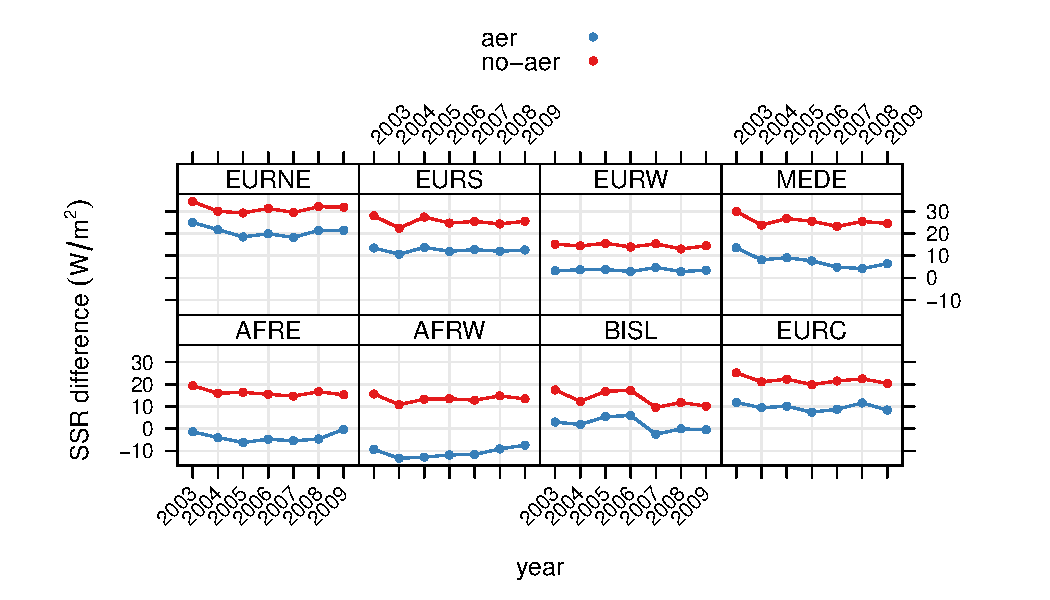
\includegraphics[width=1\textwidth]{figs/capitulo6/dif_model_sat_zonas.pdf}
\caption[Differences between climate simulations and satellite in SSR in defined areas]{Difference in shortwave solar irradiation, SSR [$\si{\watt\per\metro\squared}$], between simulations and the satellite aggregated by areas defined in figure \ref{fig:mapapral} in the period 2003-2009.}
\label{fig:figura4}
\end{figure}

In order to calculate the impact on photovoltaic production, shortwave solar irradiation, SSR, from the climate model simulations and the satellite dataset is used as an input of the photovoltaic model. For a fixed typology of the panels, the difference between simulations with respect to the satellite dataset as input, in the mean of daily productivity for each month, is represented in Figure \ref{fig:ciclosFixed}. The productivity is defined as the energy production per unit of power installed $\si{\kilo\wattpeak}$.

In general, The NO-AER simulation gives more production than the AER and the satellite, overestimating the PV power potential. Climate model simulations, AER and NO-AER, differ more from satellite PV production output in winter months, whereas in summer months, AER and satellite are close to each other, except for the EURNE region. This area is the most biased area of the model in comparison with the satellite, perhaps due to a bias in the cloud cover.

The regions from North Africa, AFRE and AFRW, are slightly different from the rest with a roughly constant bias curve of the the annual cycle, therefore the difference in PV production between summer and winter months is lower due to the mean latitude of the area. Besides, for these areas, the AER simulations give in summer month lower PV production values than the SAT and the NO-AER, which is not the case in the rest of the regions.

The EURS area is the one with largest amplitude between winter and summer months. For April and May, the AER simulations have small differences with the satellite simulation.

\begin{figure}[h!]
\centering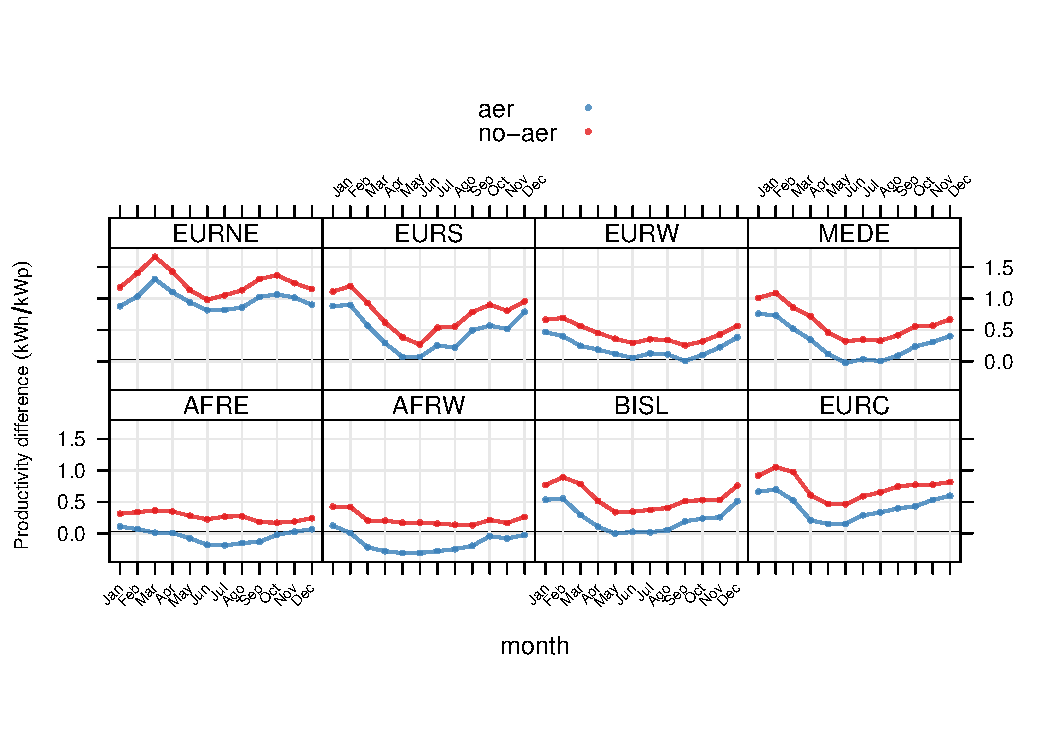
\includegraphics[width=1\textwidth]{figs/capitulo6/diferencia_mesesFIXED.pdf}
\caption[Differences in annual cycle of daily energy productivity between PV simulations with SSR from climate models andfrom satellite]{Annual cycle of daily energy productivity [$\si{\kilo\watthour\per\kilo\wattpeak}$] differences by area for the AER simulation and NO-AER simulation with respect to the satellite as inputs of the PV model, considering fixed panels.}
\label{fig:ciclosFixed}\end{figure}

\subsection{Impact of aerosols by tracking type}

\subsubsection{Mean behavior. Period 2003-2009}

In addition to the absolute difference in PV productivity between AER and NO-AER, the relative difference between simulations is presented in this section, showing the relative impact in each case. It allows us to contextualize the loss with respect of the potential of the place.

The difference in yearly PV production between both simulations, for every type of tracking panel, is represented in Figure \ref{fig:diferenciaYm}. The spatial pattern shows areas where the aerosols affect more the shortwave solar radiation. Central Europe, Po Valley and the South of the domain, along the African continent coast, are the areas where the differences are more noticeable.

For the fixed panels, the differences are around -150 $\si{\kilo\watthour\per\kilo\wattpeak}$ for some of these areas in annual terms and reaching -200 $\si{\kilo\watthour\per\kilo\wattpeak}$ in the Po Valley, Syria, Iraq and between Algeria and Tunisia.

When the two other tracking systems are considered, the difference between both simulations increases, with values of -300 $\si{\kilo\watthour\per\kilo\wattpeak}$ for the two-axes type over the most affected areas and even higher values like in the south of Turkey. These results are consistent due to the fact that the two-axes and the one-axis tracking systems are more efficient systems to give energy to the generator.

\begin{figure}[h!]
  \centering\begin{subfigure}{1\textwidth}
    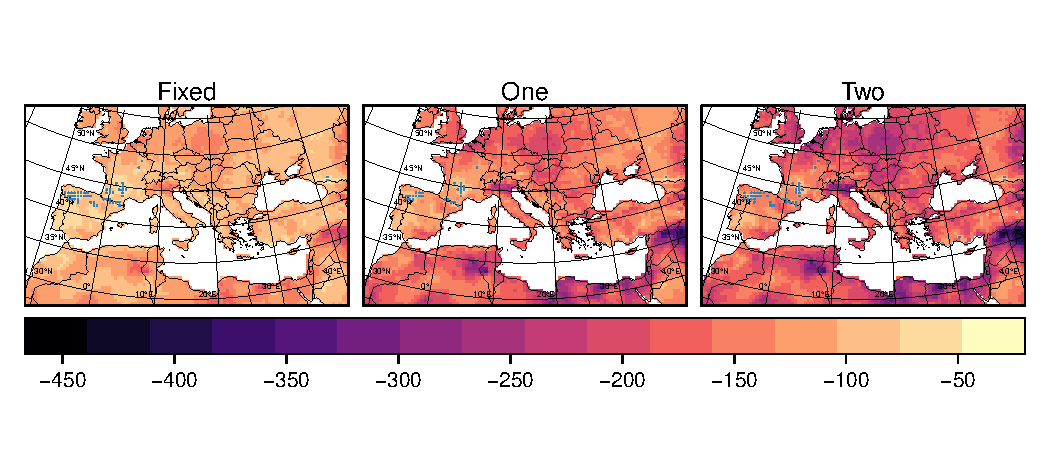
\includegraphics[width=1\textwidth]{figs/capitulo6/dif_aer_no_all_Ym20032009SIGt.pdf}
    \caption{}
    \label{fig:diferenciaYm}
  \end{subfigure}
  %
  \centering\begin{subfigure}{1\textwidth}
    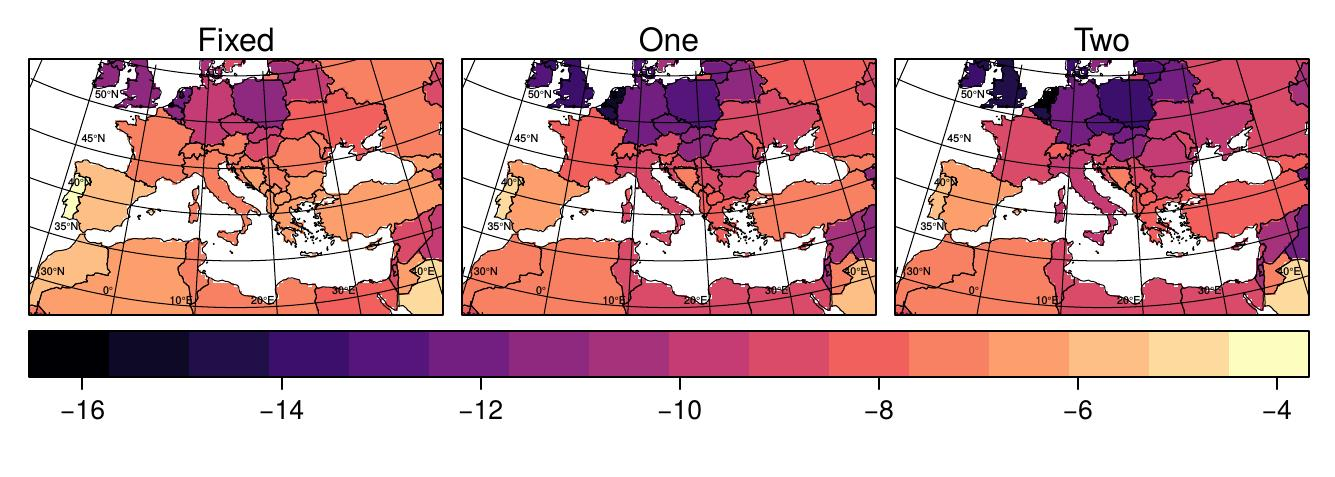
\includegraphics[width=1\textwidth]{figs/capitulo6/byCountry.jpeg}%year_all_bycountry.pdf}%{figs/RelDif_aer_no_all_Ym20032009.pdf}
    \caption{}
    \label{fig:diferenciasRel}
  \end{subfigure}
  %
  \caption[Differences in yearly PV productivity between simulations with and without aerosols]{Differences in PV yearly productivity: (a) absolute $\left[\si{\kilo\watthour\per\kilo\wattpeak}\right]$, (b) relative averaged by country (\%); for the period 2003-2009 between AER and NO-AER and for the three different types of tracking. For he non-significant differences, calculated with a 't-test', a point is over-plotted for (a)}
\end{figure}

The results of the country averages for the annual productivity are shown in Figure \ref{fig:diferenciasRel}. It is shown that the aerosols impact range from $-4\%$ to the PV production to $-16\%$. It can be seen that from the fixed panels to the one-axis, and then to the two-axes tracking type, there is an increase in the productivity losses that is more noticeable in Central Europe, like in Belgium-The Netherlands.

Germany, that has installed a high amount of PV capacity, is affected with values around $-10\%$ of loss for fixed system and more than $-12\%$ for the one-axis and two-axes panels. Thus, some countries with high PV production have moderate losses due to aerosols in relative terms. For countries in the west and south of the domain like Portugal, Spain, Morocco, Jordanian or the extension of Saudi Arabia included in the domain, the relative amount of energy loss is smaller due to its high potential, with differences between $-5\%$ and $-6\%$ for fixed panels and reaching $-8\%$ in some cases for the other types of tracking systems.

\subsubsection{Seasonal cycle}

\begin{figure}[h!]
  \centering
  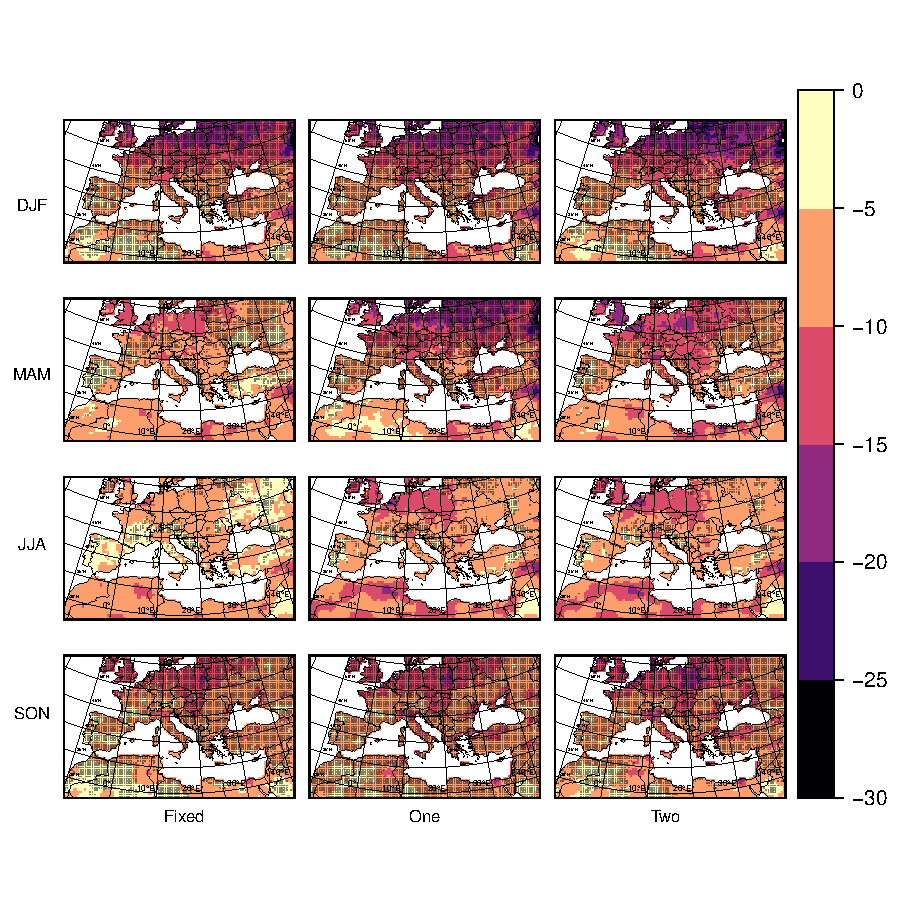
\includegraphics[width=1\textwidth]{figs/capitulo6/RelDif_aer_no_all20032009SIGt.pdf}
\caption[Differences in seasonal PV productivity between simulations with and without aerosols]{Relative difference (\%) in seasonal PV productivity between both simulation for all type of panels. For the non-significant absolute differences, calculated with a 't-test', a dot is over-plotted.}
\label{mapas}
\end{figure}

As can be seen in Figure 6.7, in seasonal terms spring (MAM) and summer months (JJA) show statistically significant values of the PV productivity difference. For winter (DJF) and Autumn (SON), there are few significant areas, mostly located in the south of the domain, in the African continent. An exception can be found for fixed panels in winter, with significant zones in Europe with values above $-10\%$, like the Po Valley or the British Islands. 

The spatial pattern for the spring season shows higher values in Central-Europe, in specific countries like Poland, Belgium and The Netherlands, or the British Islands, and in northern parts of Syria and Iraq. Maximum values in these areas, range from an impact higher than $-10\%$ for fixed panels to around $-15\%$ for the two axes tracking type. Almost the whole African part of the domain shows significant differences, with impact values above $-5\%$ and local values reaching more than $-10\%$ between Algeria and Tunisia and in areas of Libya or Egypt. 

Summer months have higher loads of aerosols over the Mediterranean. For fixed panels, only a few areas in north Africa, Middle East and north-western Europe show values with a loss higher than $-10\%$. One-axis tracking enlarge the extension of areas with a decrease higher than $10\%$ and some areas with more than $-15\%$ appear in Belgium and The Netherlands, Algeria and Syria-Iraq border. Also some smaller areas appear with PV production losses above $-15\%$ within the above mentioned areas. Between the one-axis and the two-axes tracking type, there are no substantial differences in the spatial pattern but maximum values reach in these cases $-17\%$ to $-20\%$ in the same areas.

Significance is not clearly linked to the magnitude of the relative difference in productivity. High relative differences in DJF and SON in central and northern Europe are not significant, due to the high climate variability in these areas and seasons, whereas lower relative differences in spring in Africa and in summer in southern and eastern Europe are mostly significant. The fact that JJA changes are significant over most of the domain explains the statistical significance of most yearly differences (Figure \ref{fig:diferenciaYm}), due to the high contribution of summer to the yearly production and yearly interannual variability (see e.g. \cite{Gil2015}).


\subsection{Long-term trends. Period 1980-2012}

The impact of long term trends of solar shortwave on PV production can be illustrated with the results of the simulations of the brightening period over Europe. The simulation including the aerosols dataset, NAB13, and the decreasing trend in sulfur aerosols, TREND, is able to reproduce the observed positive trend in SSR \cite*{Nabat2014}.

As a compromise between the lifetime of a PV plant and the length of the simulation, two 15-year periods (at the beginning and end of the simulated period) are evaluated as a proxy for a PV project and the potential amount of energy that can be obtained during such a project. A fixed system is selected for the panels.

The relative difference between the accumulated energy obtained by a 15-year project between 1997-2012 and energy obtained by a 15-year project between 1980-1995 can be seen in Figure \ref{fig:trends}.

\begin{figure}[h!]
  \centering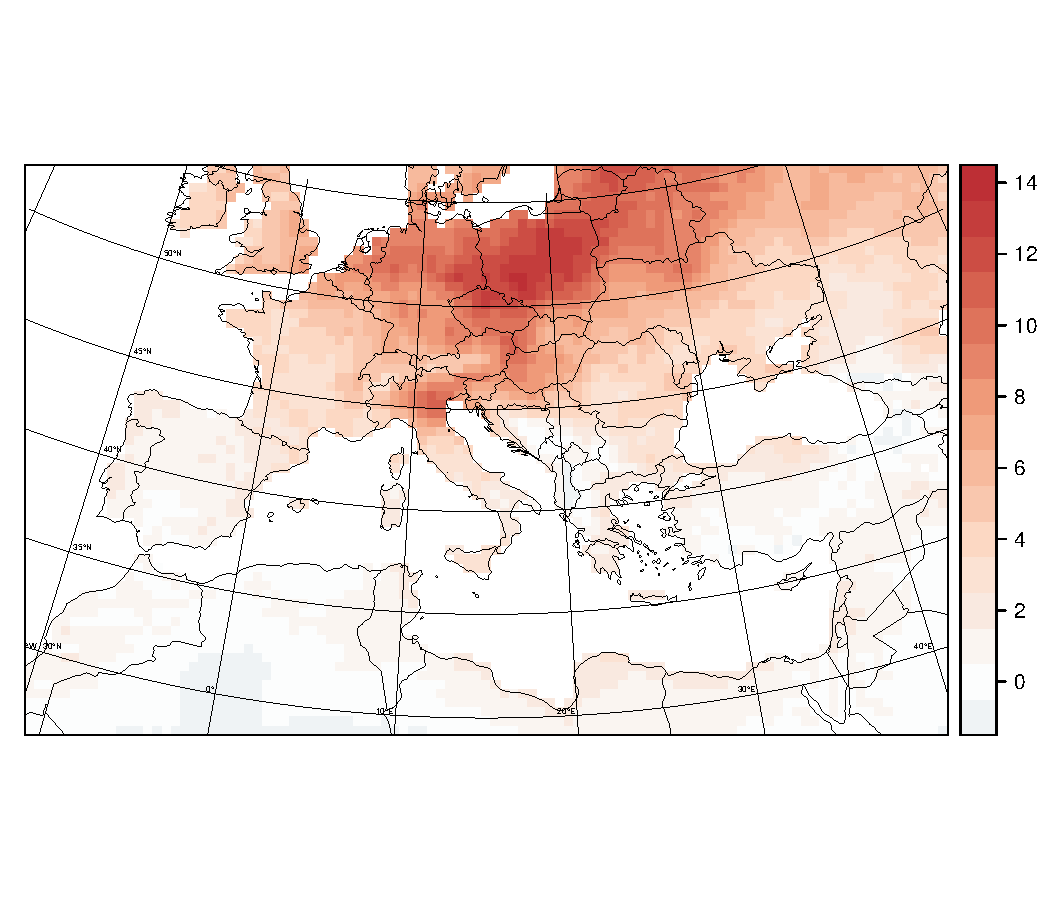
\includegraphics[width=0.7\textwidth]{figs/capitulo6/DifferencesRelativesinPVtciclo15.pdf}
\caption[Difference in PV productivity in the brightening period]{Relative difference in PV yearly productivity $[\%]$ accumulated for a 15-year period at the end and the beginning of the period: 1980-1994/1998-2012}
\label{fig:trends}
\end{figure}

In Central-Europe the differences in the energy obtained are higher, due to the fact that it is the region where anthropogenic aerosols decrease more. Accumulated over 15 years, an increase higher than 2000 $\si{\kilo\watthour\per\kilo\wattpeak}$ is found for this area. It means that about 10-14 $\%$ more energy can be produced in the lifetime of a PV plant at the end of the period.

These results highlight the impact that environmental policies could have on the PV energy production, showing that anthropogenic aerosols are able to reduce potential PV power of a project significantly. It also illustrates that future evolution of regional anthropogenic aerosols load is likely to influence expected PV production on a given site on the lifetime of a PV plant.

\section{Discussion}

\subsection{Limitations}

The coarse resolution of climate models and their bias in some variables, especially in cloud cover, makes difficult their application for solar resource assessment at local scale in most areas. However, the RCMs will evolve to finer resolution and besides, the use of climate models is mandatory to take into account future climate evolution. They are also relevant tools to perform sensitivity tests allowing to disentangle the driving factors of the resource variability such as aerosols. 

A multi-model approach would be necessary to obtain a more robust answer applying the same methodology to more models but, up to now, aerosols are poorly considered in many RCMs, which does not allow that type of study considering actual simulations. 

For the limitations in the PV model, it is important to notice that in the decomposition of SSR and the transposition to the tilted panels, some empirical relationships are used. If components of solar radiation were an output of the RCM, the additional steps for decomposition could be avoided.

It could also be pointed out that the spectral decomposition of the SSR reaching the panels would give a better input in order to calculate spectral losses of the PV modules, although for periods longer than a day the spectral effects become less significant \cite*{Martin2001}.

In the optical losses, deposition of dust over the generator surface is approximated in the assessment but could be underestimated in desert areas because it is not spatially modeled. That could mean a higher drop in transmittance and final energy production.

The time-scale is also important for the AOD representation. Several processes involving aerosols in the atmosphere are in day to weeks time-scales. We have used a realistic interannual dataset of the AOD that improves the state-of the art used in climate modeling but next studies should go further with an improvement in the aerosols representation. This will include a prognostic scheme of aerosols that allows to study finer time-scales and future scenarios, through a fully-coupled and fully-interactive aerosol-climate model. 
  

\subsection{Implications for the climate services dedicated to the energy sector }

The results show the necessity of considering aerosols in climate simulations used to deliver energy-related climate services. The inclusion of spatio-temporal variability of aerosols in RCMs may change the current estimates of future PV production over Europe \cite*{Jerez2015}. An accurate ensemble of models is essential for bridging the gap between services providers and potential users considering that some of the discrepancies between model simulations could come from the aerosols inclusion.

\subsection{PV production data issue}

The scarcity of real power data at PV plant sites is an important issue that has to be overcome in order to improve research in the fields of PV forecasting, climate services or energy modeling. The potential synergies between research institutions and different stakeholders of the energy sector will enhance the PV integration, the management and planning operations as well as the efficiency of the overall system and its development. Not only production data are needed, but also, accurate metadata will be extremely important in order to integrate into the modeling chain important factors such as: days of maintenance activities, cleaning-panel days, installed capacity, electrical characteristics of the PV power plant, among others.

\section{Conclusions}

Two main questions are addressed in this chapter: first, the evaluation of the capacity of an RCM to produce reliable estimations of PV production over the Mediterranean area. Secondly, the role of aerosols in PV production using sensitivity tests performed with the RCM. 

It is demonstrated that the use of a RCM as input of a photovoltaic production model is able to reproduce real PV data accurately at monthly time scales for two locations in the domain. Besides, the added value of including aerosols in the simulations is observed over the whole area as the simulation with aerosols shows less bias in SSR than the simulations without aerosols and it is close to the simulated PV using the satellite dataset across the whole area. 

The results show that the most impacted areas are (with some exceptions) mostly in central Europe, where the lower resource amount in combination with the influence of aerosols gives a significant reduction in potential electricity production. For the annual averaged by country productivity, the highest relative differences are around $-12\%$ for fixed typologies and are seen over Central Europe (Poland and The Netherlands). Differences increase from one axis typology to the two-axes, reaching around $-16\%$ between both simulations in Belgium and around $-13\%$ and $-14\%$ in many countries. In seasonal terms, the loss can reach values of $-20\%$ in some areas for summer months.

In the multi-decadal simulation 1980-2012 a noticeable increase in productivity has been obtained in central Europe as a result of the decreasing trend of anthropogenic aerosols observed from the end of the eighties. This trend has been associated with pollution control measures as well as economic crisis in Western Europe. This result has implications beyond the domain of this study: highly polluted countries like India and China could obtain an increase in PV productivity if pollution control policies are effectively implemented.

The non-negligible impact of aerosols on PV production in the area suggests that the inclusion of aerosols in future scenarios is necessary for solar energy assessment.

\chapter{Future projections of solar and photovoltaic  potential  in Europe\label{cha:projections}}

\begin{abstract}

  In the last decades, trends in photovoltaic deployment show an overall increase over the world and it is projected to continue growing for the next years. The comprehensive knowledge of solar resource and its future evolution is demanded by the energy sector. Solar resource and photovoltaic potential have been estimated in several studies using both global and regional climate models, showing a discrepancy between them in the sign of the projected change over Europe. An increase in surface solar radiation and in photovoltaic potential is projected by GCMs, whereas most of the RCMs simulations project a decrease. In this chapter, the role of the aerosol forcing in RCMs as a key explaining factor of this inconsistency is investigated. The results show that RCM simulations including evolving aerosols agree with GCMs in the sign and amplitude of the SSR change over Europe for mid-21st century projections (2021-2050 with respect to 1971-2000, RCP8.5). The opposite signal is projected by the rest of RCMs. The amplitude of the changes depends on the model. In terms of photovoltaic potential, RCMs including evolving aerosols simulate an important yearly increase especially in Central and Eastern Europe with  maximum values reaching +10$\%$ for some countries in summer (in one of the RCM). On the contrary, the RCMs with no evolving aerosols show a negative anomaly of PV production. This study illustrates the key role of the often-neglected aerosol forcing evolution in RCMs.% and argues for its inclusion in the next generation of the CORDEX simulations.
    
\end{abstract}

\section{Introduction}

 Due to the link between solar energy production and atmospheric variables, concern has raised about the availability of resources under climate change \cite*{Gaetani2014}. Due to that, climate modeling is a key tool to evaluate future energy potential despite some constraints like its low spatial resolution or known biases in the representation of cloudiness. 
   

% The Mediterranean region is indeed one of the regions
% which have the highest aerosol loads owing to air masses
% carrying numerous and various aerosol types (Lelieveld
% et al. 2002). These anthropogenic and natural aerosols,
% such as industrial and urban aerosols from European and
% North African towns, forest fires, biomass burning from
% eastern Europe, dust aerosols from Africa and marine
% particles, lead to strong effects on the regional radiative
% budget, climate and ecosystems of the Mediterranean
% (Rodá et al. 1993; Rosenfeld et al. 2001; Bergamo et al.
% 2008; Guieu et al. 2010). This diversity results in a large
% variety in physico-chemical and optical aerosol properties
% over the basin (Basart et al. 2009).

Attempts to estimate PV potential in the future under climate change were made in previous works \cite*{Crook2011, panagea2014, Gaetani2014, Burnett2014}. Some of them were focused locally \cite*{panagea2014, Burnett2014} and others use a single climate model \cite*{Crook2011}. Different CMIP5 simulations with different GCMs have also been evaluated to assess the photovoltaic potential under climate change conditions in \cite*{Wild2015}, projecting an increase over Europe due to the increase in clear-sky and all-sky conditions. Another sensitivity study has shown that projected increase in SSR is also augmented by changes in anthropogenic aerosols emissions for the same area \cite*{Gaetani2014}.

However, later studies using regional climate models \cite*{Jerez2015, Bartok2017} have shown the opposite behavior for some regions in Europe, an overall decrease in surface solar radiation and photovoltaic potential in the same area is projected although no significant change in cloud cover (CLT) was found. %The increase in atmospheric absorption due to the increase in water vapor content has been reported as the explanation for the decrease in SSR.

These results constitute one of the few illustrations so far of GCM-RCM inconsistency in the sign of a climate change signal \cite*{Bartok2017}. In addition, this current inconsistency may lead to diverging messages delivered to the PV production stakeholders depending on the climate information source. So far, this inconsistency has been attributed to an added-value of RCMs with respect to GCMs, due to an improved cloud representation in RCMs and therefore an improved related climate change response in RCMs \cite*{Bartok2017}.

Usually, the added value of regional climate modeling against global simulations lies on the better representation of local climate features due to the increase in resolution of coastal lines or topography that can not be solved with coarser models. However, the increase in resolution has led to a simplification of other processes in order to not compromise the computational time and resources. Many regional climate simulations have been done using a simplified representation of aerosols content, usually aerosol optical depth (AOD) climatologies without variations in time \cite*{Nabat2013, Nabat2014}, and without considering their evolution in time for future projections \cite*{Bartok2017}.

%Many regional climate simulations have been done using AOD monthly climatologies to take into account aerosol radiative forcing. Some of them have not considered any aerosols and only a few have interactive schemes \cite*{Nabat2013}. In addition, only few RCMs have considered time evolution of aerosols for future projections over Europe.


%   Despite of the fact that climate models overstimate surface solar radiation [refs] due to their bias in cloudiness representation (as it has been reported in many studies), to figure out the source of discrepancy between global and climate models is the first step to possibly project changes and trend in photovoltaic potential independently of uncertainties in magnitude.

%   Recent studies have evaluated the role of cloudiness in different sign of SSR projection [ref bartok]. The decrease in CLT for GCM per decade in the XXI century would explain the anomaly for GCM. On the other hand, RCMs do not present a significant change in CLT, and the SSR decrease is explained through the increase in atmospheric absorption.


   % simplification of other processes in order to not compromise the computational resources.


 In this context, the goals of this study are to further illustrate the GCM-RCM inconsistency by using well-chosen pairs of GCM-RCM within the Euro-CORDEX ensemble, to attribute this inconsistency to missing evolution of the aerosol forcing in CORDEX RCMs and to deliver trustable future projections of the climate-related PV potential.

In previous studies, the ensemble approach has been considered to evaluate the impact of climate change in renewable resources \cite*{Jerez2015, Tobin2018, Gil2019, Jerez2019}. However, the fact that a large majority of RCMs' simulations do not consider aerosol evolutions in their projections, the impact of aerosols is masked by the ensemble mean approaches.

In this work, we analyze the surface solar radiation (SSR) and the photovoltaic potential over Europe for the mid-21st century and the RCP8.5 scenario using GCM-RCM simulation pairs, from the Euro-CORDEX initiative. We classify different RCM simulations depending on their aerosols representation in the model and their driving GCM. A modelization chain approach is used, where SSR and temperature are the variables used as input of a photovoltaic parametric model used to calculate PV productivity.

   
   %   Although variability of solar radiation are mainly due to changes in cloudiness, in clear days other constituents of the atmosphere, mostly aerosols, decrease the amount of energy reaching the phtotovoltaic generator surface[ref]. Because of its geographical situation, the Euro-Mediterranean area is one of the most influenced areas by natural and anthropogenic aerosols coming from different sources, affecting the spatio-temporal distribution of solar resource, as explained in previous chapters and lead to strong effects on regional radiative budget.[Lieleveld, Nabat, Gutierrez]

% AOD monthly climatologies to take into account aerosol radiative  forcing,  for  example  ALADIN-Climate (Herrmann et al., 2011) and REMO (Jacob,2001). Others do not have any aerosols (e.g., RegCM-3, Artale et al., 2010; PROMES-RCM,Sanchez  et  al.,2004).  Only  few  RCMs  such  as COSMO-ART (Zubler et al.,2011a) and RegCM-4 (Giorgi et al., 2012) have interactive schemes to generate natural and anthropogenic aerosols. These interactive modules are useful for studies at the daily scale and for future climate projections (e.g.,Szopa et al.,2013). However, they might lead to biases when simulating present aerosol conditions, as the climatic biases impact the AOD field through emission, advection and wet deposition. Resorting to monthly climatologies can be justified for this reason, especially for hindcast simulations, targeting a realistic representation of the past decade 
   
  % We analyze the projections of photovoltaic potential over Europe for the RCP8.5 scenario using regional climate models simulations from EURO-CORDEX initiative \cite*{Jacob2014}. We classify different simulations attending to the aerosol representation in the model and its driving global climate model.

   Section \ref{Climate data} describes the models and simulations used in the study. A description of the aerosols datasets used by them is included here. The methodology is explained in section \ref{Methods} and the main results are explained in \ref{Results}. A discussion and a conclusion section follows.

{\section{Climate data}\label{Climate data}}

\subsection{CMIP5}

The Coupled Model Intercomparison Project Phase Five provides and coordinates global climate simulations from different modeling groups \cite*{Taylor2012} of around the world, using more than 40 models. Different RCP (Representative Concentration Pathway) scenarios are used for radiative forcing of each simulation of CMIP5. In this work, two climate models from CMIP5 are the driving models of different RCMs evaluated in the study for the scenario RCP8.5.

\subsection{Euro-CORDEX}

%The EURO-CORDEX (Jacob et. al 2014) initiative started as a 'branch' from the Coordinated Regional Climate Downscalling, CORDEX, whose aim is to provide regional climate simulations in different domains. EURO-CORDEX develops climate projections focused on the European continent at different horizontal resolutions (0.44º, 0.11º). These simulations are driven by different CMIP5 GCMs (Taylor et. al 2012).
%Despite of the known fact that aerosols have a strong influence on climate due to its direct and indirect effects, its representation in regional climate modeling has been rather limited, therefore, its impacts remains still uncertain [Nabat 2015]. ESTO EN REALIDAD ESTÁ EN EL CAPÍTULO ANTERIOR.

Euro-CORDEX develops climate projections focused on the European continent at different horizontal resolutions (0.44º, 0.11º). These simulations are driven by different CMIP5 GCMs \cite*{Taylor2012}.

Among the whole list of simulations included in the Euro-CORDEX database, aerosols are described very differently depending on the RCM. RCMs use different aerosol datasets, different levels of complexity for their representation and different temporal evolutions. In particular, most of the Euro-CORDEX RCMs do not present evolving aerosols in the future projections. Only two RCMs (namely RACMO22E and ALADIN53) include an aerosol dataset that evolves depending on the year, following the chosen RCP scenarios and the driving GCM.

For our purpose a relevant 6-member ensemble is used, which is a sub-sampling of the whole list of the 0.11° Euro-CORDEX scenario simulations performed under the RCP8.5 hypothesis. Two driving GCMs (EC-EARTH and CNRM-CM5) and four RCMs (RACMO22E, ALADIN53, CCLM4-8-17 and RCA4) are selected. Each GCM drives three RCM simulations, one with evolving aerosols and two with constant aerosols (see Table \ref{tb:families} for a detailed description of the GCM-RCM pairs). A group of three RCM simulations driven by the same GCM will be called ``family''. Although a small number of the possible Euro-CORDEX GCM-RCM pairs is used, it is largely enough to serve the purpose of the study.

To measure the climate change signal, a 30-year near-future period (2021-2050) is compared to the end of the 20th century (1971-2000). The focus on the near-future allows our results to be nearly independent of the chosen socio-economic scenario (here RCP8.5) and to maximize the aerosol effect with respect to the GHG effect. The choice of 30-year long periods allows to minimize the uncertainty related to the natural climate variability as only one realization of each GCM-RCM pair is usually computed in Euro-CORDEX. In addition, the PV power plants operating during 2021-2050 are the ones that will be planned shortly, so the results are timely for the industry.

\begin{table}[h]
\footnotesize
\begin{tabular}{>{\raggedrigth}m{4.5cm}>{\raggedright}m{3cm}>{\raggedright}m{3cm}}
\toprule 
CMIP5 GCM & Institution  & RCM  \tabularnewline
\midrule
CNRM-CERFACS-CNRM-CM5 & CNRM & ALADIN53 \tabularnewline
&CLMcom&CCLM4-8-17\tabularnewline 
&SMHI&RCA4\tabularnewline
\midrule  
ICHEC-EC-EARTH&KNMI&RACMO\tabularnewline
&CLMcom&CCLM4-8-17\tabularnewline
&SMHI&RCA4\tabularnewline
%\midrule  
%HadGEM2-ES&KNMI&RACMO\tabularnewline
%&CLMcom&CCLM4-8-17\tabularnewline
%&SMHI&RCA4\tabularnewline  
\bottomrule
%  \br
\end{tabular}\\
\caption[RCMs from Euro-CORDEX grouped by the CMIP5 GCMs drivers generating the 2 families of simulations studied]{\label{tb:families}RCMs from Euro-CORDEX grouped by the CMIP5 GCMs drivers generating the 2 families of simulations studied.}
\end{table}
\normalsize

%**La tabla de la descripción de aerosoles de bartok de los GCM se puede referenciar y hacer la de aerosoles de EURO-CORDEX (o de los modelos que yo utilizo?)


\subsection{Aerosols datasets}

% Among the whole list of simulations included in the Euro-CORDEX database, aerosols are described differently depending on the RCM considered. Each RCM includes a different aerosols dataset in the evaluation runs that can be also applied for future projections, including the time evolution following the correspondent RCP scenario. Simpler approaches consist of a fixed climatology that is also included on the future projections but without evolving in time. There are other RCMs that do not include any aerosols dataset in their simulation runs.

The information about the aerosols datasets included in the regional climate simulations from Euro-CORDEX, used in this chapter has been included in Table \ref{tb:aero}. %Only two RCMs include time evolving aerosols for the scenario projections: RACMO22e and ALADIN5.3. %Each of these RCMs uses a different aerosols dataset. Whereas ALADIN5.3 select the Szopa dataset, RACMO22E uses the CAM inventory (Lamarqué et al).

% AEROSOLES EN LOS GCM! On the other hand, both driving GCMs used prescribed aerosols from Lamarqué inventory (2010

\begin{table}[h!]
\footnotesize
\begin{tabular}{>{\raggedrigth}m{1.3cm}>{\raggedright}m{1.5cm}|>{\raggedright}m{2.2cm}>{\raggedright}m{2.2cm}>{\raggedright}m{2cm}}
\toprule 
Institution  & RCM & description & classes & scenarios \tabularnewline
\midrule
CNRM & ALADIN53 & Climatology. Szopa 2013 & 5 classes: sea salt, sulfate,black carbon, desert dust,organic carbon.& evolve with RCP \tabularnewline
CLMcom&CCLM4-8-17& Climatology. Tanré 1984 & 4 classes: sea, land, desert, urban.& no evolution\tabularnewline 
SMHI&RCA4& Parametrization in radiation fluxes & Single integrated class.& no evolution \tabularnewline
KNMI&RACMO&CAM inventory, Lamarque 2010 & 6 classes: sulfate, organic matter, desert dust, sea salt,stratospheric aerosols, volcanic & evolve with RCP\tabularnewline
\bottomrule
%  \br
\end{tabular}\\
\caption[RCMs from Euro-CORDEX and aerosols description]{\label{tb:aero}RCMs from Euro-CORDEX and aerosols description.}
\end{table}
\normalsize

\subsubsection{Aerosols description in ALADIN53}

The aerosols dataset used for ALADIN53 runs is based on AOD fields including 5 different species: black carbon, organic carbon, dust, sea salt, and sulfate. It is described in \cite*{Szopa2013} and built from the global LMDz-OR-INCA Climate-Chemistry coupled model. For the historical period it takes into account reference aerosol emissions, including seasonal cycle for each species and trends for the anthropogenic aerosol species. The future simulations include the same temporal variations but following the corresponding RCP8.5 scenario emissions. 

\subsubsection{Aerosols description in RACMO22E}

A spatial and vertically distributed dataset derived from CAM-inventory \cite*{Lamarque2010} is used in RACMO22E simulations. It also accounts for the same five different species. The historical run also follows the reference emissions \cite*{Lamarque2010} and from 2006 it evolves in time with the RCP.

The resulting changes in AOD for both models in summer months (JJA) between 2021-2050 and a reference period 1971-2000, are represented in Figure \ref{fig:aod} . An overall decrease for both models is observed with the maximum change in central Europe and with a slightly smaller signal for the RACMO22E simulation.

\begin{figure}[h!]
\centering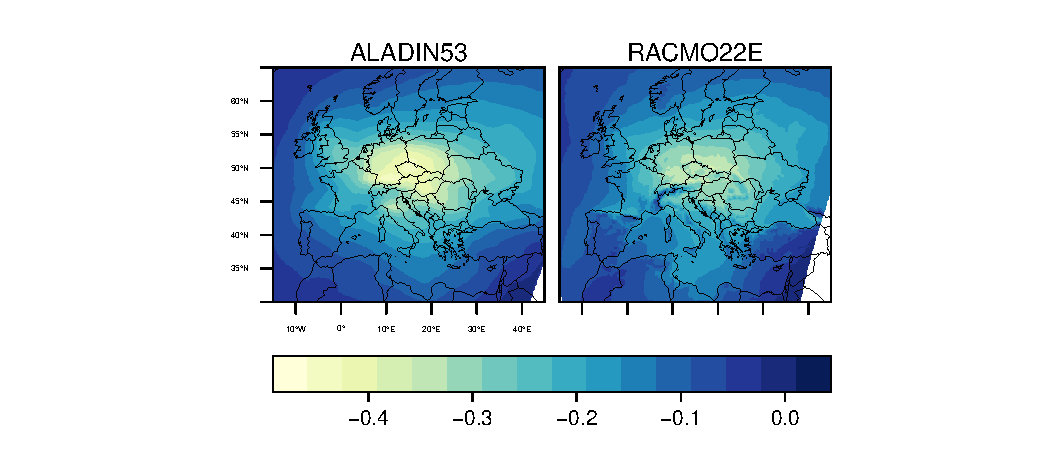
\includegraphics[width=1\textwidth]{figs/capitulo7/ANOMALIAS_JJA_AOD_2050-2021_r12.pdf}
\caption[Aerosol optical depth summer change between 2050-2021 with respect to 1971-2000 over Europe]{Aerosols Optical Depth summer changes between 2021-2050 with respect to the period 1971-2000 for ALADIN53 and RACMO22E models.}
\label{fig:aod}
\end{figure}

{\section{Methods}\label{Methods}}

\subsection{Spatial analysis}

In order to analyze the spatial behavior of solar radiation, SSR, the summer mean change for the period 2021-2050 with respect to the reference period 1971-2000 is calculated. Summer months, June, July and August, JJA, correspond to the season when the AOD (aerosols optical depth) is higher over Europe and the Mediterranean area \cite*{Lelieveld}.

% The 2021-2050 period has been selected because of two reasons: in the mid-century the effects of global warming are still not very remarkable among the simulations, which could help to better detect the impact of including evolving aerosols. On the other hand, the PV power plants operating during 2021-2050 are the ones that will be planned shortly, so the results are presently relevant for the industry.

As an important driver of the variability of SSR the same procedure is applied to the total cloud cover variable, CLT. This allows to know if a correlation exists between both changes and how is modified between models with or without evolving aerosols.

% \subsubsection{Linear regression}

% In second order, it has been investigated the linear relationship of the mean spatial anomalies of SSR and CLT for each simulation. For the models including evolving aerosols, the AOD anomaly is also included for a multivariate linear regression model, following equation \ref{eq:linear}:

% \begin{equation}
%   \Delta{SSR}=\alpha\Delta{CLT}+\beta\Delta{AOD}+\gamma
% \label{eq:linear}
% \end{equation}

%{\color{red} No he añadido esta parte aún porque rompe un poco la coherencia del capítulo, pero este me parece el mejor lugar para poner estos resultados. ¿Estáis de acuerdo?}

\subsection{PV potential}

In order to obtain a projection of the photovoltaic productivity over Europe under climate change scenarios, the modeling chain approach explained in the previous chapters is considered. Solar radiation from the different climate simulations, SSR, is used as an input of the photovoltaic model that gives an estimation of the power output as explained in chapter \ref{cha:methods}.

%The two steps followed in the modeling process of the photovoltaic output are: first, to calculate solar irradiation reaching solar cells, afterwards the electrical performance of the system is modeled (through the procedure explained in chapter 4 of this manuscript).

The PV modeling process can be summarized in two steps: first, incident solar irradiation that reaches solar cells inside the panels is obtained through the decomposition of global solar irradiation and the transposition to the plane-of-array (POA). After that, the electrical performance of the system is modeled. Surface solar irradiation from climate models is equivalent to global irradiation at the horizontal plane, G(0).

Monthly means of surface solar radiation, SSR, from climate models is decomposed first into the diffuse and beam components. The decomposition is made through a regression between the clearness index \cite*{Liu1960} (which represents the relationship between global irradiation at the horizontal plane and the extra-terrestrial irradiation) and the diffuse fraction (relationships between the diffuse component and G(0)) \cite*{Page1961}.

A monthly average daily profile of the irradiance $\left[\si{\watt\per\metro\squared}\right]$ is obtained for each month \cite{Collares-Pereira1979} which allows to obtain different components in the plane of the array. Direct irradiance in the tilted plane is obtained straightforwardly from geometrical criteria. The diffuse component is obtained using the Hay and McKay model \cite{hay1985estimating}.

The effective irradiation is then obtained from the consideration of optical losses due to the incident angle and dust accumulation \cite{Martin2001}. Only a moderate dust accumulation degree is considered.

The second step transforms the ‘effective’ irradiation into power output $\left[\si{\kilo\watthour\per\kilo\wattpeak}\right]$ considering the electrical performance of the system. The system includes characteristics of a general PV module and inverter, the arrangement of the generator and some efficiency losses. Characteristics of the general PV system are the same as the ones described in chapter \ref{cha:methods}.

Yearly PV potential changes for the period 2021-2050 with respect to the reference period 1971-2000 are computed. Yearly values of productivity are considered a good estimation of the performance of a power plant and are considered as a reference for feasibility studies and finance calculations.

Changes in PV potential production for summer months are also calculated, considering that it is the season with higher loads of aerosols and it is when solar energy production peaks.

{\section{Results}\label{Results}}

\subsection{Changes in SSR and CLT}

The summer (JJA) mean changes of the period 2021-2050 with respect to the reference period 1971-2000 is represented in Figure \ref{fig:anomalySSR} and Figure \ref{fig:anomalyCLT} first for surface solar irradiation, SSR, and then for total cloud cover, CLT.

\begin{table}[h!]
\footnotesize
\begin{tabular*}{1\textwidth}{@{}lllllll}
\br
  CMIP5 GCM & RCM & $\Delta{SSR}$ & $\Delta{CLT}$ & $\Delta{AOD}$ & $\rho_{SSR,CLT}$  & $\rho_{SSR,AOD}$\\
\midrule 
%\mr  
  CNRM-CERFACS-CNRM-CM5& & 9.9 & 0.5 & & -0.4 &  \\
            &ALADIN53 & 12.6 & 0.3 & -0.2 & -0.2 & -0.9\\
            &CCLM4-8-17& -2.4 & -0.8 & - & -0.7 & -  \\
            &RCA4& -2.6 & 0.2 & - & -0.8 & - \\
\midrule
%\mr   
  ICHEC-EC-EARTH& &5.6 & -0.3 & &-0.3 &  \\
          &RACMO& 4.8 & 0.5 & -0.1 & -0.3 & -0.6 \\
          &CCLM4-8-17& -2.7 & -0.9 & - & -0.8 & - \\
          &RCA4&-2.1 & 0.1 & - & -0.8 & - \\
\bottomrule
%\br
\end{tabular}\\
  \caption[Changes of SSR, CLT, AOD and spatial correlations]{\label{tb:spatial correlations}Spatial changes with respect of the reference period for SSR (W/m²), CLT (\%) and AOD; and spatial correlation between SSR,CLT and AOD changes maps.}
\end{table}
\normalsize
 
% \begin{table}[h!]
% \caption[SSR, CLT and AOD anomalies and spatial correlations over Europe]{\label{tb:spatial correlations}SSR, CLT and AOD anomalies and spatial correlations between them.}
% \footnotesize
% \begin{tabular*}{0.8\textwidth}{@{}lllllll}
% \br
% CMIP5 GCM & RCM & $\rho_{SSR,CLT}$  & $\rho_{SSR,AOD}$ & $\Delta{SSR}$ & $\Delta{CLT}$ & $\Delta{AOD}$\\
% \midrule 
% %  \mr  
%   CNRM-CM5& & & & 3.73 & 0.73 & \\
%             &ALADIN5.3& -0.26 & -0.94 & 7.15 & 0.60 & -0.10\\
%             &CCLM4-8-17& -0.83 & - & -4.17 & -0.15 & - \\
%             &RCA4& -0.71 & - & -3.55 & 0.21 & - \\
% \midrule
% % \mr  
%   ICHEC-EC-EARTH& & & & 1.84 & -0.49 & \\
%           &RACMO& -0.15 & -0.65 & 2.60 & 0.13 & -0.11 \\
%           &CCLM4-8-17& -0.80 & - & -4.40 & -0.51 & - \\
%           &RCA4& -0.59 & - & -3.44 & 0.09 & - \\
% \bottomrule
% %  \br
% \end{tabular}\\
% \end{table}
% \normalsize

% \begin{figure}
% \centering
% \tabskip=0pt
% \valign{#\cr
%   \hbox{%
%     \begin{subfigure}[b]{.4\textwidth}
%     \centering
%     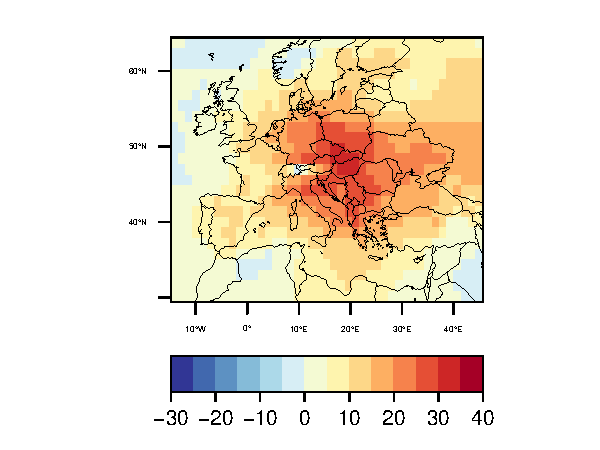
\includegraphics[height=4cm, width=\textwidth]{figs/capitulo7/CNRM-CM5_ANOMALIAS_JJA_SSR_2050-2021.pdf}
%     \caption{Figure 1}
%     \end{subfigure}%
%   }\vfill
% %  \noalign{\hfill}
%   \hbox{%
%     \begin{subfigure}{.4\textwidth}
%     \centering
%     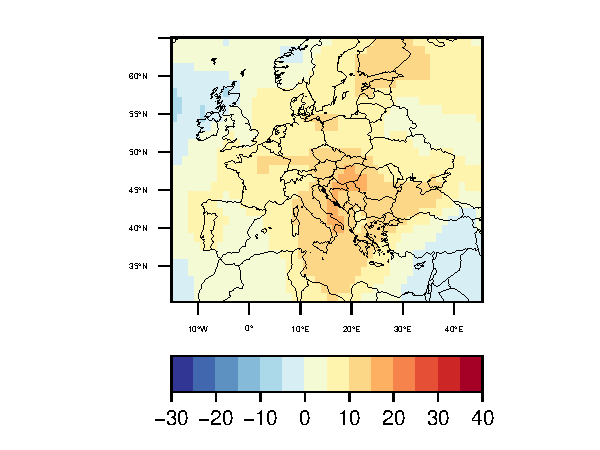
\includegraphics[height=4cm,width=\textwidth]{figs/capitulo7/EC-EARTH_ANOMALIAS_JJA_SSR_2050-2021.pdf}
%     \caption{Figure 2}
%     \end{subfigure}%
%   }\cr
%   \hbox{% 
%     \begin{subfigure}{.6\textwidth}
%     \centering
%     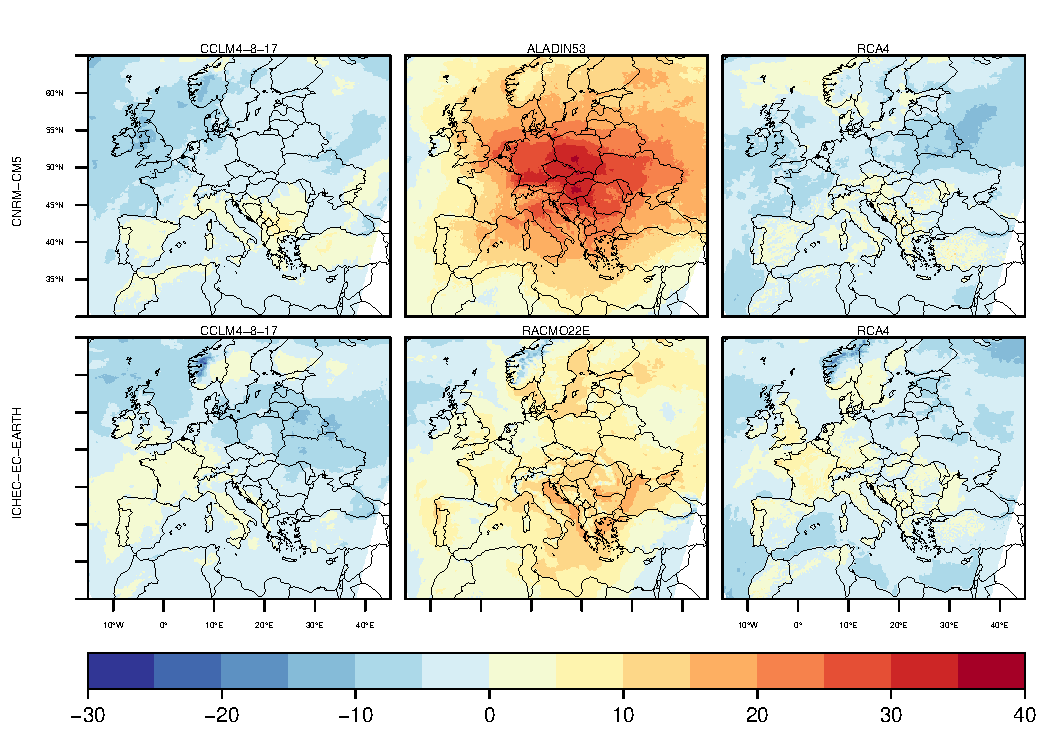
\includegraphics[width=\textwidth]{figs/capitulo7/ANOMALIAS_JJA_SSR_2050-2021_r12.pdf}
%     \caption{Figure 3}
%     \end{subfigure}%
%   }\cr
% }
% \caption{Full caption}
% \end{figure}

\begin{figure}[h]
  \centering\begin{subfigure}{0.4\textwidth}
    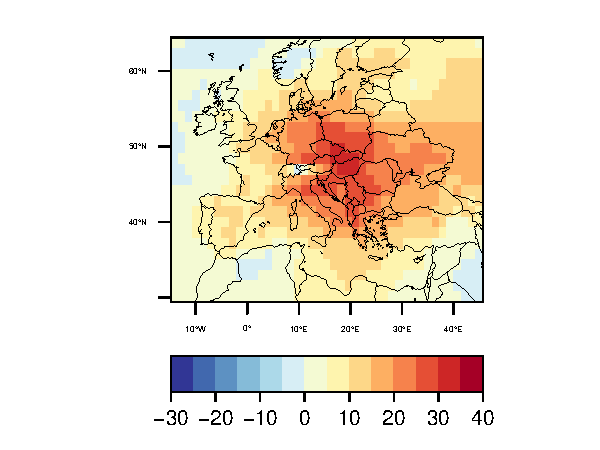
\includegraphics[width=1.4\textwidth]{figs/capitulo7/CNRM-CM5_ANOMALIAS_JJA_SSR_2050-2021.pdf}
    \caption{CNRM-CM5}
  \end{subfigure}
  %
  \centering\begin{subfigure}{0.4\textwidth}
    \includegraphics[width=1.4\textwidth]{figs/capitulo7/EC-EARTH_ANOMALIAS_JJA_SSR_2050-2021.pdf}\hfill
    \caption{EC-EARTH}
  \end{subfigure}
\hspace{0.1mm}
  %
  \centering\begin{subfigure}{1\textwidth}  
    \includegraphics[width=1\textwidth]{figs/capitulo7/ANOMALIAS_JJA_SSR_2050-2021_r12_names.pdf}
    \caption{Families of RCMs simulations. First row driven by CNRM-CM5 and second row driven by EC-EARTH.}
  \end{subfigure}
  \caption[Summer mean SSR change over Europe for the period 2021-2050 with respect of 1971-2000 with different climate models]{Mean change 2021-2050 with respect to the reference period 1970-2021 of JJA surface solar radiation, SSR. $\left[\si{\watt\per\metro\squared}\right]$}
\label{fig:anomalySSR}
\end{figure}
 
Summer mean change shows an increase in Europe, more relevant in Central-Europe, for regional climate models with evolving aerosols in scenarios (ALADIN53 and RACMO22E) although there are differences in the magnitude of the changes. ALADIN53 presents the highest change in the mentioned area, which correlates with the negative change and spatial pattern of AOD of this model, as can be seen in Figure \ref{fig:aod}. For RACMO, the AOD change has a similar spatial pattern but the magnitude is slightly smaller. The projected SSR changes in RACMO are positive for a large area among the domain although they do not reach the higher values of ALADIN53. Mean values for the whole domain are positive for ALADIN (12.6 $\si{\watt\per\metro\squared}$) and RACMO (4.8 $\si{\watt\per\metro\squared}$) and negative for the others.

The rest of the RCMs from the first and second family present a similar signal in SSR among them, with a slight decrease in SSR with the exception of southern and western Europe that show a small increase.

The changes projected in the two RCMs that account for the evolution of aerosols in the future agree in the sign with the projected changes of the two GCM of the respective families also represented in Figure \ref{fig:anomalySSR}. The magnitude and the spatial pattern of the changes in CNRM-CM5 coincide with the ones in ALADIN53. In the same manner, the driving GCM of the second family, EC-EARTH, also presents similar changes to RACMO22E. 

\begin{figure}[h]
  \centering\begin{subfigure}{0.4\textwidth}
    \includegraphics[width=1.4\textwidth]{figs/capitulo7/CNRM-CM5_ANOMALIAS_JJA_CLT_2050-2021.pdf}
    \caption{CNRM-CM5}
  \end{subfigure}
  %
  \centering\begin{subfigure}{0.4\textwidth}
    \includegraphics[width=1.4\textwidth]{figs/capitulo7/EC-EARTH_ANOMALIAS_JJA_CLT_2050-2021.pdf}\hfill
    \caption{EC-EARTH}
  \end{subfigure}
  \hspace{0.1mm}
  %
  \centering\begin{subfigure}{1\textwidth}  
    \includegraphics[width=1\textwidth]{figs/capitulo7/ANOMALIAS_JJA_CLT_2050-2021_r12_names.pdf}
\caption{Families of RCMs simulations. First row driven by CNRM-CM5 and second row driven by EC-EARTH.}
\end{subfigure}
\caption[Change in summer CLT over Europe for the period 2021-2050 with respect of 1971-2000 with different climate models]{Mean change 2021-2050 with respect to the reference period 1970-2021 of JJA total cloud cover, CLT. [\%]}
\label{fig:anomalyCLT}      
\end{figure}

In general, for the whole domain, the mean change in CLT is close to zero for every simulation as can be seen in Table \ref{tb:spatial correlations}. The spatial pattern of CLT change in ALADIN53 shows a positive sign in the area where the change in SSR is higher (Central Europe), which is remarkable. For ALADIN53 and RACMO22E the spatial correlation between CLT and SSR is very low, -0.2 and -0.1 respectively, whereas it increases between SSR and AOD, -0.9 for ALADIN53 and -0.6 for RACMO22E.

On the whole, the spatial pattern of CLT explains well the spatial pattern of SSR in RCMs without evolving aerosols whereas both AOD and CLT are required to explain spatial pattern of SSR in GCMs and RCMs with evolving aerosols. The spatial pattern of AOD is even the dominant signal for ALADIN53.


%** Hablar de que la anomalía de nubosidad es parecida entre modelos independientemente de su GCM?

% \begin{figure}[h!]
% \centering\includegraphics[width=1\textwidth]{figs/capitulo7/ANOMALIAS_JJA_AOD_2050-2021_r12.pdf}
% \caption{Mean anomaly 2021-2050 with respect to the reference period 1970-2021 of JJA AOD}
% \label{fig:anomalyAOD}
% \end{figure}


\subsection{Projected changes in PV production}

The photovoltaic yearly productivity, defined as the power output by the power installed, is calculated for each pixel of land in the domain of Euro-CORDEX. Then, the averaged by country difference with respect to the reference period 1971-2000 is represented in Figure \ref{fig:pvcountry}. 

\begin{table}[h!]
\footnotesize
\begin{tabular*}{1.1\textwidth}{@{}llll|llllll}
\br
CMIP5 GCM & RCM &  $\Delta{PV_{annual}}$ & $\Delta{PV_{JJA}}$ & Spain & Germany & Italy & Greece & Hungary & Czech &&&&&&&&&&Republic\\
\midrule 
%\mr   
  \\CNRM-CM5&ALADIN53& 3.2$\%$ & 2.7 $\%$ & 2.4$\%$ & 10.9$\%$ & 6.3$\%$ & 4.6$\%$ & 11.2$\%$ & 12.0$\%$ \\
          &CCLM4-8-17& -1.4$\%$ & -0.8$\%$ & -0.6$\%$ & -2.2 $\%$ & -0.4$\%$ & 0.3 $\%$ &-1.0$\%$ &-1.6$\%$ \\
          &RCA4& -1.5$\%$ & -0.7 $\%$ & -0.8 $\%$ & -1.5 $\%$ & -0.4 $\%$ & -0.4$\%$ &  -0.5$\%$ &-1.1$\%$ &\\
\midrule
%\mr  
  \\EC-EARTH &RACMO& -0.6$\%$ & 0.6$\%$ & 0.3$\%$ & 1.4$\%$ & 1.6$\%$ & 2.3$\%$ & 4.0$\%$ &2.5$\%$\\
                 &CCLM4-8-17& -2.3$\%$ & -1.5$\%$ & -0.6$\%$ & -1.8$\%$ & -0.6$\%$ & -1.4$\%$ & -1.8$\%$ &-1.7$\%$\\
                 &RCA4& -2.0$\%$ & -0.7$\%$ & -0.8$\%$ & -0.3$\%$ & -0.6$\%$ & -0.9$\%$ & -0.7$\%$ &-0.4$\%$\\
\bottomrule
%\br
\end{tabular}\\
\caption{\label{tb:pvanomalies}Relative change of yearly PV [\%] and JJA PV [\%] with respect of the reference period for the whole domain and JJA PV relative change averaged by country [\%].}
\end{table}
\normalsize


% \begin{table}[h!]
% \caption[Future PV anomalies for Europe and averaged by country]{\label{tb:pvanomalies}PV projected relative anomalies for Europe and averaged by country.}
% \footnotesize
% \begin{tabular*}{1\textwidth}{@{}llll|llll}
% \br
% CMIP5 GCM & RCM &  $\Delta{PV_{annual}}$ & $\Delta{PV_{JJA}}$ & Spain & Germany & Italy & Greece\\
% \midrule 
% %  \mr  
%   CNRM-CM5&ALADIN5.3& 2.2$\%$ & 3.3 $\%$ & 2.45$\%$ & 10.89$\%$ & 6.44$\%$ & 4.63$\%$ \\
%           &CCLM4-8-17& -2.8$\%$ & -1.8$\%$ & -0.63$\%$ & -2.26 $\%$ & -0.42$\%$ & 0.28 $\%$\\
%           &RCA4& -2.6$\%$ & -2.0 $\%$ & -0.77 $\%$ & -1.51 $\%$ & -0.42 $\%$ & -0.37 $\%$\\
% \midrule
% % \mr  
%   ICHEC-EC-EARTH &RACMO& -0.9$\%$ & 0.4 $\%$ & 0.35$\%$ & 1.37$\%$ & 1.63$\%$ & 2.35$\%$\\
%                  &CCLM4-8-17& -3.9$\%$ & -2.5 $\%$ & -0.55$\%$ & -1.94$\%$ & -0.58$\%$ & -1.4$\%$\\
%                  &RCA4& -3.6$\%$ & -2 $\%$ & -0.83$\%$ & -0.34$\%$ & -0.57$\%$ & -0.91$\%$\\
% \bottomrule
% %  \br
% \end{tabular}\\
% \end{table}
% \normalsize

%{\color{red} Anomalía para los modelos con aerosoles y los modelos sin aerosoles}

The geographical dependence of the PV potential change is due to the spatial pattern of SSR change, which is closely related to the anomaly of AOD in central Europe projected by ALADIN53 and RACMO22E. The most important result is that the projected change in PV output is positive for both RCMs with evolving aerosols in countries where the other RCMs show the opposite sign. This suggests that for some areas in Europe information from RCMs projections might not be accurate if an ensemble is used for these energy related purposes.

\begin{figure}[h!]
    \includegraphics[width=1\textwidth]{figs/capitulo7/bycountryYEAR_newscript.pdf}
    \caption[Yearly change of PV productivity over Europe for the period 2021-2050 with respect of 1971-2000]{Yearly change of PV productivity for 2021-2050 with respect to the reference period 1970-2021 $\left[\si{\kilo\watthour\per\kilo\wattpeak}\right]$}
        \label{fig:pvcountry}
\end{figure}


The annual values of PV relative change for the models without aerosol evolution is between -2.3 to -1.4$\%$ over the whole domain. ALADIN53 projects a positive annual mean change of 3.2$\%$ and RACMO22E of, -0.6$\%$. In absolute terms, values above 100 $\left[\si{\kilo\watthour\per\kilo\wattpeak}\right]$ are found for countries in Central Europe for ALADIN53 and in norht-eastern countries, values are lower than $-50$ $\left[\si{\kilo\watthour\per\kilo\wattpeak}\right]$ for models not including aerosols evolution, as can be seen in Figure \ref{fig:pvcountry}.
%It is important to notice that for the ALADIN53 simulation including aerosols the sign in PV power output anomaly is positive and negative in the other cases. !!Besides, the RACMO anomaly is close to zero (although negative) whereas the rest of the simulation has the same magnitude order of the anomaly: ~ -2 to -4\%

For summer months, which is the most important season for solar energy supply, the results are shown in Figure \ref{fig:pvcountryjja}. In this case, the same pattern as in the annual PV yield is found, with the two models with evolving aerosols showing higher changes. All the simulations not including evolving aerosols have very similar values, close to zero in western and southern Europe a slightly negative for the rest of the countries. On the other hand, ALADIN53 gives an strong change for Central-Europe and countries with a maximum that ranges between 11-13\% of increase. RACMO22E has positive values but smaller in magnitude with the maximum values around the eastern-southern European countries.

\begin{figure}[h!]
    \includegraphics[width=1\textwidth]{figs/capitulo7/bycountryJJArelative_area_newscriptall5.pdf}
    \caption[JJA mean relative change of PV productivity over Europe for the period 2021-2050 with respect of 1971-2000]{PV JJA mean change of 2021-2050 with respect to the reference period 1970-2021 $\left[\%\right]$}
\label{fig:pvcountryjja}
\end{figure}

At the country level, some representative ones have been included in Table \ref{tb:pvanomalies}. For ALADIN53 values above 10$\%$ are found in Germany, Hungary, and the Czech Republic, whereas lower values are found for Spain (2.4$\%$), Italy (6.3$\%$) or Greece (4.6$\%$), although still positive. In the same countries, RACMO22E shows the highest increase in Hungary, 4$\%$,  and smaller values in the rest, from 0.3$\%$ in Spain to 2.4$\%$ in the Czech Republic.
 
%Uncertainties due to the different AOD datasets used in the two RCMs and in the radiative transfer code of the model difficults the robust answer about the change magnitude. Averaging the results for the non-aerosols simulations and aerosols simulation, we obtain the results in fugure.


\section{Discussion}

To determine the uncertainty in climate projections is one of the main issues in climate science because the information underlying the simulations is difficult to communicate. In order to isolate the uncertainty sources in a multi-model work it is necessary to design a sensitivity test for each of the models in the study. Up to now, there are not enough simulations from the Euro-CORDEX ensemble including evolving aerosols and for those that include them, there is not the same simulation excluding the aerosols forcing, in order to quantify its impact.

For that reason, this preliminary study, although it highlights very important issues, is the firs step in order to understand the role of aerosols in the RCM projections. Uncertainties due to the different AOD datasets used in the two RCMs and in the radiative transfer code of the model difficult the robust answer about the change magnitude. 

In addition, although an overestimation of SSR from climate models has been reported extensively, the seek for a robust answer in trends or in the sign in PV potential projected changes justifies the use of climate projections independently from these constraints. They should be undoubtedly addressed later in order to improve the message for potential users and stakeholders of the energy industry.

\section{Conclusion}

The study shows that regional climate models with evolving aerosols in the scenarios behave differently to those that have an aerosols climatology constant in time. In model using evolving aerosols, the sign of the SSR change is reversed, agreeing with the positive signal projected by their driving GCMs. This result is a relevant contribution to the explanation of the disagreement found in previous studies between GCMs and RCMs in the sign of future SSR change.
% and the magnitude of the anomaly is important yearly and in summer months. The most impacted countries are those in Central-Europe.

It has been shown also that the change of SSR is not directly linked with change in CLT in the case of the RCMs simulations that include evolving aerosols. The spatial correlation between SSR and CLT in these models is very low and AOD changes are needed to explain the SSR changes.

These results have been derived from the mid of the XXI century. Different changes could be found at the end of the century when the climate change signal is higher.

The results show a general small decrease of SSR for RCMs with no-evolving aerosols, more important in higher latitudes that barely affects the future of PV production, as was pointed out in previous studies \cite*{Jerez2015, Jerez2019}. However, for ALADIN53 and RACMO22E simulations, a general positive signal in PV projections is found in Central-Europe in the first case and in Southern-Eastern Europe for the second one.

%The magnitude of the anomaly depends on the country, being the most impacted areas those in Central-Europe, with an important potential increase of more than 10\% in Germany or around 6\% in Italy. A more limited but still positive increase, between 3 and 5\%, is projected the east and south-east of Europe

% In summer months the relative mean change projected for PV is above 10$\%$ in Germany, Poland, Austria etc. and maximum values between 3 and 5$\%$ are also projected in the East and South-East of Europe (for the models with evolving aerosols).  

The study shows that regional climate models with time evolving aerosols in the scenario runs behaves different than those that have a fixed climatology. The sign of the anomaly is reversed (for summer mean anomalies), agreeing with the positive signal in PV potential projected by GCMs. The magnitude od the anomalies depends on the country, being the most impacted those in Central-Europe and southern Europe. There is also a small decresase for RCMs with no-evolving aerosols, more important in higher latitudes. 

We can conclude that the impact of evolving aerosols on the SSR projections, could affect PV potential projections significantly. Insofar the uncertainty in aerosols datasets and schemes used in RCMs can be narrowed, more accurate projections could be achieved for the energy sector. The fact of the reversed signal in mid century for the PV anomalies in the case of simulations including evolving aerosols, highlights the risk of using an ensemble mean for renewable energy projections and the lack of a robust answer for now.   


%\begin{subappendices}

\section*{Appendix B}

\subsection*{Significance of PV changes in Euro-CORDEX}

The statistical significance of the changes of PV potential has been calculated for each simulation. Results of the significance after a t-test and with a threshold of the p-value of 0.05 are represented in Figure \ref{fig:pvalor}

\begin{figure}[h]
    \includegraphics[width=1\textwidth]{figs/capitulo7/pvalor_prueba.pdf}
    \caption[Statistical significance of PV changes]{Significance of the PV differences between 2021-2050 with respect to the reference period 1970-2021 using a t-test. Red color is for significant results and blue color for no significant.}
\label{fig:pvalor}
\end{figure}

Significant values are found in ALADIN53 for the whole domain with the exception of certain areas in North-Africa. For the other models in the same family, CCLM and RCA4, the extension of significant areas is smaller. In the last one, significant differences are found in eastern Europe, the North-African continent and some dispersed areas like the British Islands and France. For the CCLM4-8-17 the differences are significant in the north of the African continent, the British Islands and some areas in the continental Eastern-Europe and the south of the Scandinavian Peninsula.

In the second family, driven by the EC-EARTH model, significant differences for the RACMO22E model are less extended than for the other simulations. The significant values are around the south-east of Europe, which correspond to the area of higher PV change. The spatial pattern of significant differences of CCLM and RCA4 is very similar, with significant values in the south of the domain, Eastern Europe and the North of the Scandinavian countries. For RCA4 significant values are also found over the IP. 

\subsection*{Med-CORDEX analysis}

As part of the CORDEX initiative, scientific groups involved in Med-CORDEX \cite*{Ruti2016} project provide simulations around the Mediterranean area over a domain that is slightly different to the one used in Euro-CORDEX (see Figure \ref{fig:cordexdomain}). An important characteristic in Med-CORDEX ensemble with respect to the Euro-CORDEX is that they provide atmosphere-ocean coupled simulations. A coupled simulation is able to reproduce interactive fluxes between the sea surface and the atmosphere, which will improve the representation of certain climate characteristics, specially in an area like the Mediterranean Sea.

A first look into the Med-CORDEX simulations through an analysis  similar to the one developed in the previous chapter is shown in the next section. However, the Med-CORDEX ensemble is limited and only few simulations allow us to apply the pairwise or family comparison principle used before.

\subsubsection*{Climate models}

The only model available with aerosols evolution for scenarios in the Med-CORDEX ensemble is ALADIN-RCSM4 \cite*{Sevault2014}. In order to isolate the uncertainties coming from the GCMs forcing, RCMs forced with CNRM-CM5 are selected to be compared with ALADIN RCSM4. Only one model apart from ALADIN uses CNRM-CM5 as boundary conditions, the PROTHEUS RCM \cite*{Artale2010}

The scenario RCP4.5 is the only available for the 2 models. The reference period is 1971-2000 and the future period is 2021-2050 as above.

\subsubsection*{Scenario RCP4.5 of relevant variables}

The change of SSR and CLT for summer months with respect to the reference period is represented for the two model simulations.

\begin{figure}[h!]
    \includegraphics[width=0.8\textwidth]{figs/capitulo7/diferences_ssr_medcordex.pdf}
    \caption[Summer SSR change over Med-CORDEX domain for the period 2021-2050 with respect of 1971-2000 with different climate models]{SSR change [$\si{\watt\per\metro\squared}$] for the period 2021-2050 with respect to the reference period 1971-2000}
    \label{fig:medcordexssr}
\end{figure}

The spatial pattern of SSR change is different in the two simulations. The ALADIN-RCSM4 shows a generalized increase over the domain with values around 10 $\si{\watt\over\metro\squared}$ and reaching 15 $\si{\watt\over\metro\squared}$  in certain areas. For PROTHEUS, the spatial pattern shows negative changes in the North of the domain. Positive values are around 5 $\si{\watt\over\metro\squared}$ in the Southern part of Europe with some areas of 10 $\si{\watt\over\metro\squared}$. The south-western area of the domain, which roughly corresponds to the IP, shows the highest values of change, close to 15 $\si{\watt\over\metro\squared}$.

\begin{figure}[h!]
    \includegraphics[width=0.8\textwidth]{figs/capitulo7/diferences_clt_medcordex.pdf}
    \caption[Summer CLT change over Med-CORDEX domain for the period 2021-2050 with respect of 1971-2000 with different climate models]{CLT change [$\%$] for the period 2021-2050 with respect to the reference period 1971-2000}
\label{fig:medcordexclt}
\end{figure}

In Figure \ref{fig:medcordexclt} the change in CLT for the two models can be seen with respect to the reference period. In this case in opposition to the change in SSR, the spatial pattern of both models is similar, projecting a decrease of CLT for the Mediterranean area and a slight increase in Central to Northern Europe. Nevertheless, the decrease of CLT in ALADIN-RCSM4 is smaller.

Differences in spatial pattern suggest that there are other factors affecting the resource change in RCP4.5 projections. Spatial correlation between these variables is presented in Table \ref{tb:medcordexspcor}.

Mean change for the whole domain is larger for ALADIN-RCSM4 than for PROTHEUS, but the CLT mean change is similar for both. The spatial correlation between CLT and SSR is highly negative for PROTHEUS and less negative for ALADIN-RCSM4.

\begin{table}[H]
\footnotesize
\begin{tabular*}{0.8\textwidth}{@{}llllllll}
\br
& $\rho_{SSR,CLT}$  & $\rho_{SSR,AOD}$ & $\Delta{SSR}$ & $\Delta{CLT}$  \\
\midrule
ALADIN-RCSM4& -0.61 & -0.66 & 6.83 & -1.17 \\
PROTHEUS& -0.90 & - &  0.67& -1.76 \\
\bottomrule
\end{tabular}\\
\label{tb:medcordexspcor}
\caption[Changes in SSR, CLT and spatial correlation for Med-CORDEX models]{\label{tb:medcordexspcor}Changes in SSR (W/m²), CLT (\%) and spatial correlation between them.}
\end{table}
\normalsize
 
\subsection*{Final comments}

Differences between changes in both climate models indicate that changes in SSR are not only influenced by cloudiness. In addition to the analyses developed in chapter 7, these preliminary results show that a deeper research on how aerosols influence future projections of solar resource should be done, air-sea coupling may also affect changes in SSR indirectly. The results from CORDEX initiative FPS-AEROSOLS, will help to reduce the uncertainty in surface solar radiation future projections, helping in the application of solar energy modeling for the future. 

A deeper study on coming simulations from the Med-CORDEX ensemble can be and important contribution to complete the work presented in this chapter, showing differences with the non-coupled models and it is expected to be done in future research.
%\end{subappendices}

% \end{document}